%! BibTeX Compiler = biber
\documentclass{article}
\usepackage{xcolor}
\definecolor{BLUELINK}{HTML}{0645AD}
\definecolor{DARKBLUELINK}{HTML}{0B0080}
\definecolor{LIGHTBLUELINK}{HTML}{3366BB}
\definecolor{PURPLELINK}{HTML}{663366}
\PassOptionsToPackage{hyphens}{url}
\usepackage[colorlinks=false ]{hyperref}
% for linking between references, figures, TOC, etc in the pdf document
\hypersetup{colorlinks,
linkcolor=DARKBLUELINK,
anchorcolor=DARKBLUELINK,
citecolor=DARKBLUELINK,
filecolor=DARKBLUELINK,
menucolor=DARKBLUELINK,
urlcolor=BLUELINK
} % Color citation links in purple
\PassOptionsToPackage{unicode}{hyperref}
\PassOptionsToPackage{naturalnames}{hyperref}

\usepackage[margin=60pt]{geometry}
\usepackage{amssymb,amsfonts,amsmath,amsthm,mathtools}
\usepackage{lmodern}
\usepackage{bm,bbold}
\usepackage{verbatim}
\usepackage{float}
\usepackage{listings, enumerate, enumitem}
\usepackage[export]{adjustbox}
\usepackage{tabu}
\usepackage{longtable}
\tabulinesep=0.6mm
\newcommand\cellwidth{\TX@col@width}
\usepackage{hhline}
\setlength{\arrayrulewidth}{1.2pt}
\usepackage{multicol,multirow,array}
\usepackage{etoolbox}
\AtBeginEnvironment{tabu}{\footnotesize}
\usepackage{booktabs}

\usepackage{graphicx}
\graphicspath{{artworks/}}
\makeatletter
\def\input@path{{artworks/}}
\makeatother
\pdfstringdefDisableCommands{%
\renewcommand*{\bm}[1]{#1}%
% any other necessary redefinitions
}
\newcommand{\specialcell}[2][c]{%
    \begin{tabular}[#1]{@{}c@{}}#2\end{tabular}}

\usepackage{xfrac, nicefrac}
\usepackage[backend=biber,style=nature]{biblatex}
\addbibresource{codon_models.bib}
\pdfinclusioncopyfonts=1

\begin{document}
\part*{Supplementary materials}
\tableofcontents
 
\pagebreak

\section{Rate of adaptation enrichment}
\subsection{Method summary}

\begin{center}
    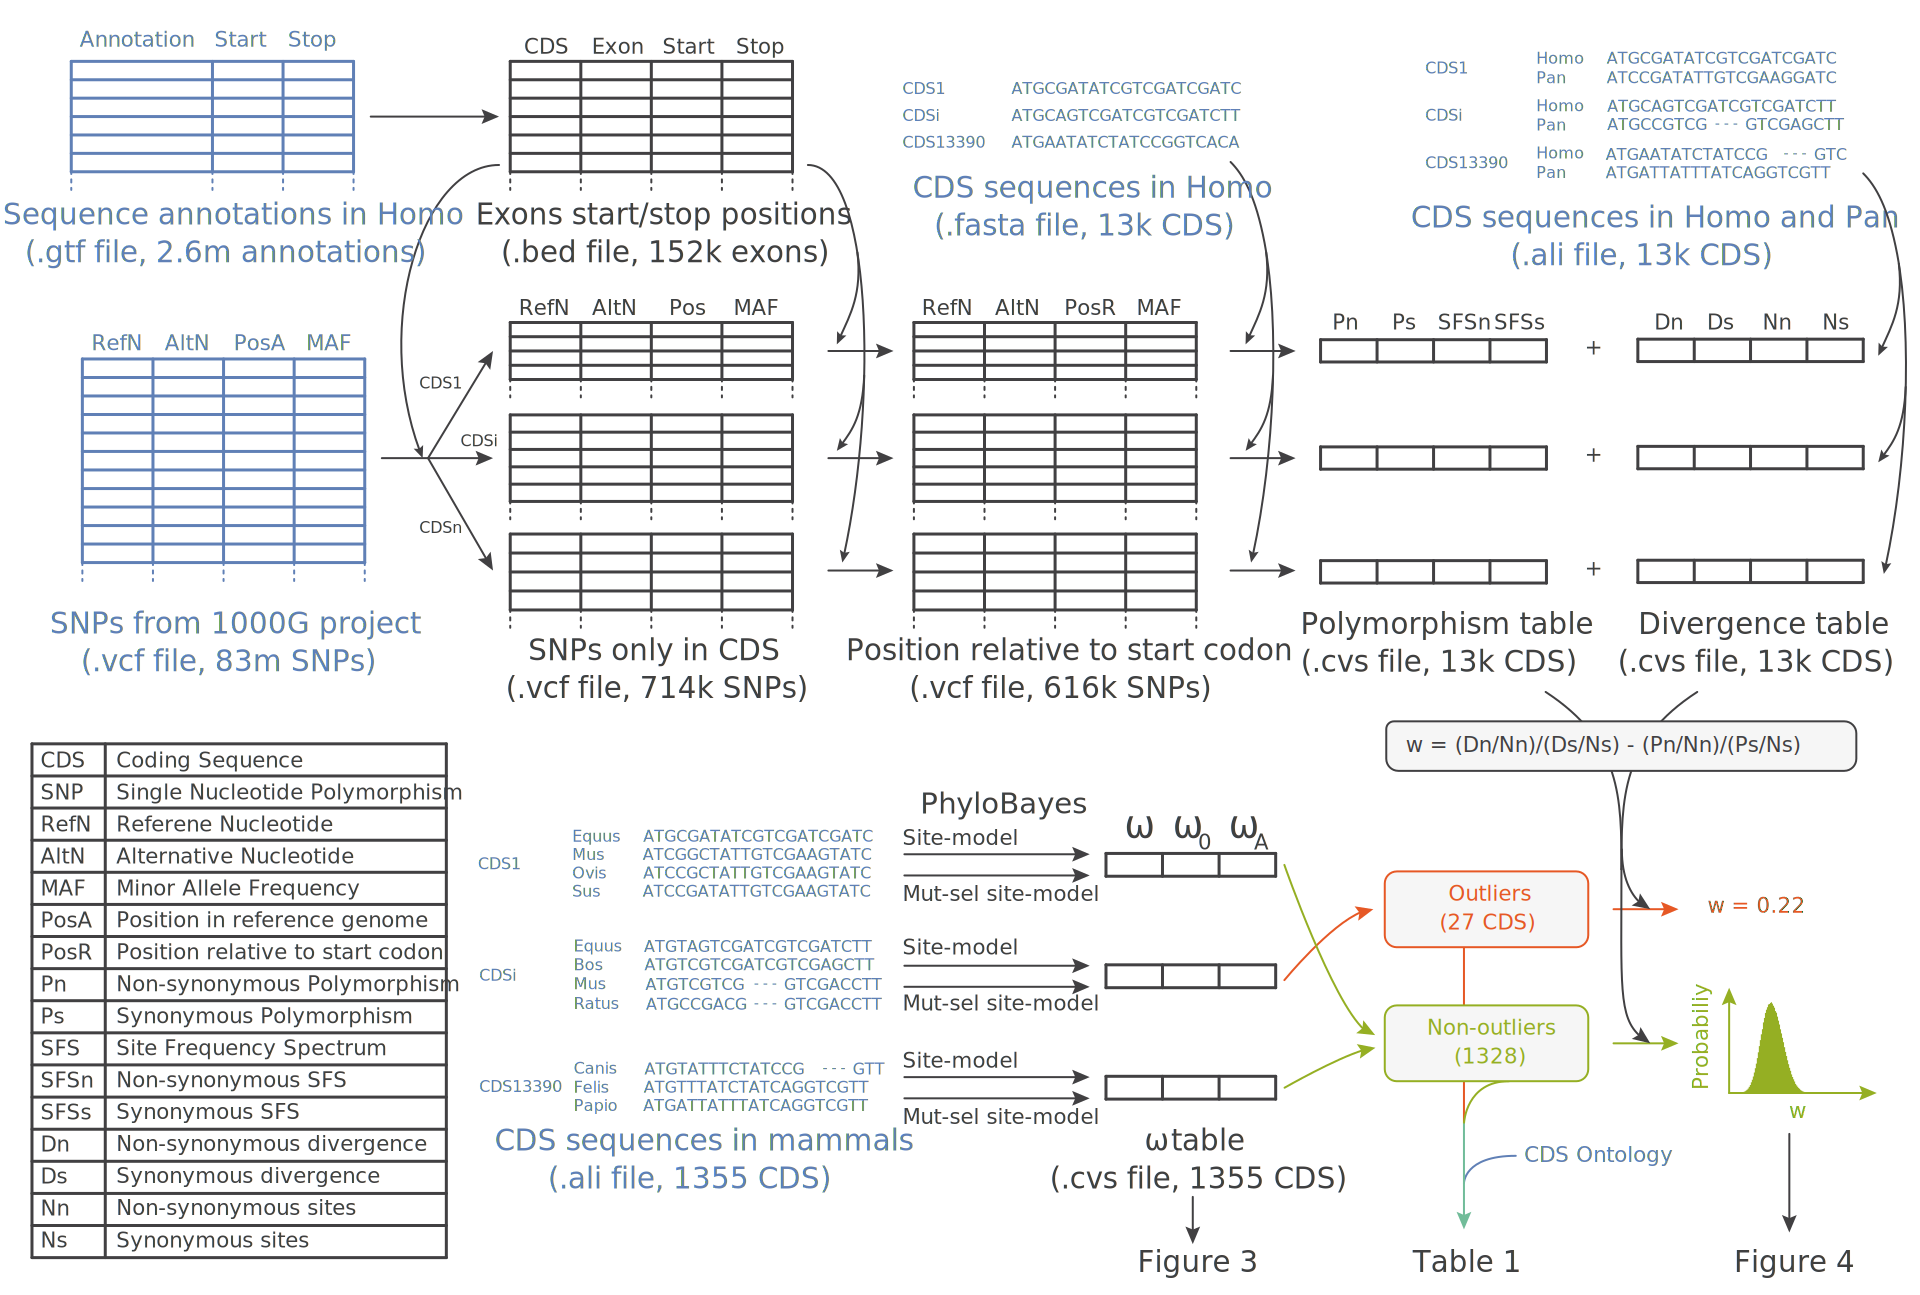
\includegraphics[width=\linewidth]{pipeline}
\end{center}

\subsection{Comparison - MK/PolyDFE/grapes}

\begin{center}
    \includegraphics[width=\linewidth]{results.pval}
    \includegraphics[width=\linewidth]{results.delta_wa} \\
    $\Delta \omega_{\text{A}} = \omega_{\text{A}}^{\text{Adaptive set}} - \omega_{\text{A}}^{\text{Nearly-neutral set}}$
\end{center}

\subsection{Folded SFS at gene level - grapes} 
\begin{center}
\includegraphics[width=\linewidth]{ViolinPlot/gene-folded-grapes.pdf} 
\begin{adjustbox}{width = 1\textwidth}
\begin{tabular}{llrrrrrrrrr}
\toprule
             Species &                Population & $\omega_{\textrm{A}}^{\textrm{S}}$ & $\omega_{\textrm{NA}}^{\textrm{S}}$ & $\omega^{\textrm{S}}$ & $\alpha^{\textrm{S}}$ & $\omega_{\textrm{A}}^{\textrm{N}}$ & $\omega_{\textrm{NA}}^{\textrm{N}}$ & $\omega^{\textrm{N}}$ & $\alpha^{\textrm{N}}$ &       p-value \\
\midrule
          Bos taurus &                      IRBT &                              0.126 &                               0.225 &                 0.351 &                 0.358 &                              0.163 &                               0.255 &                 0.418 &                 0.390 &         1.000 \\
          Bos taurus &                      UGBT &                              0.146 &                               0.206 &                 0.352 &                 0.414 &                              0.169 &                               0.252 &                 0.421 &                 0.401 &         1.000 \\
 Chlorocebus sabaeus &                  Barbados &                              0.237 &                               0.149 &                 0.386 &                 0.614 &                              0.142 &                               0.277 &                 0.419 &                 0.340 & 4.3e$^{-195}$ \\
 Chlorocebus sabaeus &  Central African Republic &                              0.169 &                               0.226 &                 0.395 &                 0.428 &                              0.157 &                               0.267 &                 0.424 &                 0.370 &   2.2e$^{-5}$ \\
 Chlorocebus sabaeus &                  Ethiopia &                              0.140 &                               0.256 &                 0.396 &                 0.353 &                              0.152 &                               0.273 &                 0.424 &                 0.358 &         1.000 \\
 Chlorocebus sabaeus &                    Gambia &                              0.160 &                               0.224 &                 0.384 &                 0.417 &                              0.121 &                               0.294 &                 0.416 &                 0.292 &  4.4e$^{-33}$ \\
 Chlorocebus sabaeus &                     Kenya &                              0.221 &                               0.180 &                 0.401 &                 0.552 &                              0.153 &                               0.276 &                 0.429 &                 0.356 &   5e$^{-152}$ \\
 Chlorocebus sabaeus &                     Nevis &                              0.153 &                               0.230 &                 0.384 &                 0.400 &                              0.111 &                               0.305 &                 0.416 &                 0.267 &  4.2e$^{-42}$ \\
 Chlorocebus sabaeus &               Saint Kitts &                              0.186 &                               0.197 &                 0.382 &                 0.486 &                              0.120 &                               0.294 &                 0.415 &                 0.290 &  9.1e$^{-88}$ \\
 Chlorocebus sabaeus &              South Africa &                              0.213 &                               0.176 &                 0.388 &                 0.548 &                              0.141 &                               0.278 &                 0.420 &                 0.337 & 5.4e$^{-142}$ \\
 Chlorocebus sabaeus &                    Zambia &                              0.217 &                               0.177 &                 0.395 &                 0.551 &                              0.154 &                               0.270 &                 0.424 &                 0.363 & 1.1e$^{-103}$ \\
        Homo sapiens &                       AFR &                              0.194 &                               0.272 &                 0.466 &                 0.416 &                              0.168 &                               0.351 &                 0.519 &                 0.322 &  2.8e$^{-14}$ \\
        Homo sapiens &                       AMR &                              0.168 &                               0.297 &                 0.465 &                 0.361 &                              0.129 &                               0.389 &                 0.518 &                 0.249 &  3.7e$^{-21}$ \\
        Homo sapiens &                       EAS &                              0.162 &                               0.303 &                 0.466 &                 0.349 &                              0.149 &                               0.370 &                 0.519 &                 0.286 &   1.8e$^{-5}$ \\
        Homo sapiens &                       EUR &                              0.167 &                               0.298 &                 0.465 &                 0.359 &                              0.140 &                               0.379 &                 0.519 &                 0.269 &    6e$^{-11}$ \\
        Homo sapiens &                       SAS &                              0.200 &                               0.265 &                 0.465 &                 0.430 &                              0.122 &                               0.397 &                 0.519 &                 0.235 &  1.4e$^{-67}$ \\
          Ovis aries &                      IROA &                              0.233 &                               0.120 &                 0.353 &                 0.659 &                              0.178 &                               0.220 &                 0.397 &                 0.447 &  1.1e$^{-80}$ \\
          Ovis aries &                      IROO &                              0.248 &                               0.106 &                 0.353 &                 0.701 &                              0.175 &                               0.223 &                 0.398 &                 0.439 &   3e$^{-134}$ \\
          Ovis aries &                      ISGC &                              0.243 &                               0.109 &                 0.352 &                 0.690 &                              0.173 &                               0.224 &                 0.396 &                 0.435 & 1.2e$^{-104}$ \\
\bottomrule
\end{tabular}
\end{adjustbox}
\end{center}
\subsection{Folded SFS at site level - grapes} 
\begin{center}
\includegraphics[width=\linewidth]{ViolinPlot/site-folded-grapes.pdf} 
\begin{adjustbox}{width = 1\textwidth}
\begin{tabular}{llrrrrrrrrr}
\toprule
             Species &                Population & $\omega_{\textrm{A}}^{\textrm{S}}$ & $\omega_{\textrm{NA}}^{\textrm{S}}$ & $\omega^{\textrm{S}}$ & $\alpha^{\textrm{S}}$ & $\omega_{\textrm{A}}^{\textrm{N}}$ & $\omega_{\textrm{NA}}^{\textrm{N}}$ & $\omega^{\textrm{N}}$ & $\alpha^{\textrm{N}}$ &       p-value \\
\midrule
          Bos taurus &                      IRBT &                              0.276 &                               0.376 &                 0.652 &                 0.423 &                              0.225 &                               0.438 &                 0.663 &                 0.338 &  6.6e$^{-62}$ \\
          Bos taurus &                      UGBT &                              0.325 &                               0.331 &                 0.656 &                 0.495 &                              0.188 &                               0.477 &                 0.665 &                 0.281 & 1.5e$^{-193}$ \\
 Chlorocebus sabaeus &                  Barbados &                              0.531 &                               0.163 &                 0.694 &                 0.765 &                              0.216 &                               0.462 &                 0.678 &                 0.318 & 1.1e$^{-267}$ \\
 Chlorocebus sabaeus &  Central African Republic &                              0.279 &                               0.424 &                 0.702 &                 0.396 &                              0.178 &                               0.505 &                 0.683 &                 0.259 & 1.2e$^{-116}$ \\
 Chlorocebus sabaeus &                  Ethiopia &                              0.358 &                               0.340 &                 0.698 &                 0.513 &                              0.181 &                               0.501 &                 0.682 &                 0.264 & 6.6e$^{-181}$ \\
 Chlorocebus sabaeus &                    Gambia &                              0.355 &                               0.340 &                 0.695 &                 0.510 &                              0.187 &                               0.492 &                 0.678 &                 0.275 &   3e$^{-158}$ \\
 Chlorocebus sabaeus &                     Kenya &                              0.286 &                               0.416 &                 0.702 &                 0.407 &                              0.144 &                               0.543 &                 0.688 &                 0.209 & 2.3e$^{-234}$ \\
 Chlorocebus sabaeus &                     Nevis &                              0.236 &                               0.459 &                 0.695 &                 0.338 &                              0.184 &                               0.495 &                 0.679 &                 0.269 &  2.7e$^{-47}$ \\
 Chlorocebus sabaeus &               Saint Kitts &                              0.250 &                               0.446 &                 0.695 &                 0.358 &                              0.127 &                               0.550 &                 0.677 &                 0.186 & 2.2e$^{-209}$ \\
 Chlorocebus sabaeus &              South Africa &                              0.245 &                               0.454 &                 0.699 &                 0.349 &                              0.212 &                               0.468 &                 0.680 &                 0.310 &    2e$^{-15}$ \\
 Chlorocebus sabaeus &                    Zambia &                              0.211 &                               0.489 &                 0.700 &                 0.300 &                              0.235 &                               0.450 &                 0.685 &                 0.343 &         1.000 \\
        Homo sapiens &                       AFR &                              0.288 &                               0.442 &                 0.729 &                 0.394 &                              0.312 &                               0.478 &                 0.790 &                 0.394 &         0.998 \\
        Homo sapiens &                       AMR &                              0.297 &                               0.432 &                 0.729 &                 0.407 &                              0.317 &                               0.473 &                 0.790 &                 0.401 &         0.991 \\
        Homo sapiens &                       EAS &                              0.334 &                               0.396 &                 0.730 &                 0.458 &                              0.296 &                               0.495 &                 0.791 &                 0.373 &    8e$^{-10}$ \\
        Homo sapiens &                       EUR &                              0.285 &                               0.445 &                 0.730 &                 0.390 &                              0.283 &                               0.507 &                 0.790 &                 0.358 &         0.235 \\
        Homo sapiens &                       SAS &                              0.286 &                               0.443 &                 0.729 &                 0.392 &                              0.298 &                               0.492 &                 0.790 &                 0.377 &         0.890 \\
          Ovis aries &                      IROA &                              0.342 &                               0.282 &                 0.624 &                 0.548 &                              0.200 &                               0.453 &                 0.652 &                 0.306 & 1.1e$^{-176}$ \\
          Ovis aries &                      IROO &                              0.394 &                               0.231 &                 0.625 &                 0.630 &                              0.217 &                               0.437 &                 0.654 &                 0.331 & 1.2e$^{-201}$ \\
          Ovis aries &                      ISGC &                              0.368 &                               0.257 &                 0.625 &                 0.588 &                              0.223 &                               0.428 &                 0.652 &                 0.343 & 1.4e$^{-161}$ \\
\bottomrule
\end{tabular}
\end{adjustbox}
\end{center}
\subsection{Unfolded SFS at gene level - grapes} 
\begin{center}
\includegraphics[width=\linewidth]{ViolinPlot/gene-unfolded-grapes.pdf} 
\begin{adjustbox}{width = 1\textwidth}
\begin{tabular}{llrrrrrrrrr}
\toprule
             Species &                Population & $\omega_{\textrm{A}}^{\textrm{S}}$ & $\omega_{\textrm{NA}}^{\textrm{S}}$ & $\omega^{\textrm{S}}$ & $\alpha^{\textrm{S}}$ & $\omega_{\textrm{A}}^{\textrm{N}}$ & $\omega_{\textrm{NA}}^{\textrm{N}}$ & $\omega^{\textrm{N}}$ & $\alpha^{\textrm{N}}$ &       p-value \\
\midrule
          Bos taurus &                      IRBT &                              0.120 &                               0.273 &                 0.393 &                 0.305 &                              0.189 &                               0.276 &                 0.465 &                 0.406 &         1.000 \\
          Bos taurus &                      UGBT &                              0.130 &                               0.267 &                 0.397 &                 0.327 &                              0.168 &                               0.298 &                 0.466 &                 0.359 &         1.000 \\
 Chlorocebus sabaeus &                  Barbados &                              0.190 &                               0.206 &                 0.395 &                 0.479 &                              0.076 &                               0.352 &                 0.429 &                 0.178 & 2.7e$^{-267}$ \\
 Chlorocebus sabaeus &  Central African Republic &                              0.186 &                               0.221 &                 0.407 &                 0.456 &                              0.088 &                               0.349 &                 0.436 &                 0.201 & 1.4e$^{-249}$ \\
 Chlorocebus sabaeus &                  Ethiopia &                              0.084 &                               0.322 &                 0.406 &                 0.207 &                              0.084 &                               0.352 &                 0.436 &                 0.192 &         1.000 \\
 Chlorocebus sabaeus &                    Gambia &                              0.094 &                               0.305 &                 0.399 &                 0.236 &                              0.139 &                               0.294 &                 0.433 &                 0.322 &         1.000 \\
 Chlorocebus sabaeus &                     Kenya &                              0.206 &                               0.202 &                 0.407 &                 0.505 &                              0.080 &                               0.357 &                 0.437 &                 0.183 & 4.3e$^{-293}$ \\
 Chlorocebus sabaeus &                     Nevis &                              0.082 &                               0.313 &                 0.395 &                 0.208 &                              0.052 &                               0.376 &                 0.429 &                 0.122 &  3.6e$^{-47}$ \\
 Chlorocebus sabaeus &               Saint Kitts &                              0.108 &                               0.289 &                 0.398 &                 0.272 &                              0.081 &                               0.350 &                 0.431 &                 0.189 &  1.5e$^{-34}$ \\
 Chlorocebus sabaeus &              South Africa &                              0.162 &                               0.243 &                 0.405 &                 0.400 &                              0.115 &                               0.322 &                 0.437 &                 0.264 &  1.1e$^{-64}$ \\
 Chlorocebus sabaeus &                    Zambia &                              0.154 &                               0.252 &                 0.406 &                 0.380 &                              0.103 &                               0.335 &                 0.438 &                 0.235 &  3.9e$^{-71}$ \\
        Homo sapiens &                       AFR &                              0.204 &                               0.280 &                 0.484 &                 0.420 &                              0.175 &                               0.361 &                 0.535 &                 0.326 &  1.7e$^{-17}$ \\
        Homo sapiens &                       AMR &                              0.119 &                               0.364 &                 0.483 &                 0.246 &                              0.132 &                               0.400 &                 0.532 &                 0.247 &         1.000 \\
        Homo sapiens &                       EAS &                              0.126 &                               0.355 &                 0.481 &                 0.261 &                              0.156 &                               0.377 &                 0.532 &                 0.292 &         1.000 \\
        Homo sapiens &                       EUR &                              0.121 &                               0.360 &                 0.481 &                 0.252 &                              0.139 &                               0.394 &                 0.532 &                 0.260 &         1.000 \\
        Homo sapiens &                       SAS &                              0.163 &                               0.319 &                 0.482 &                 0.338 &                              0.129 &                               0.405 &                 0.533 &                 0.241 &  2.4e$^{-21}$ \\
          Ovis aries &                      IROA &                              0.204 &                               0.162 &                 0.366 &                 0.557 &                              0.135 &                               0.277 &                 0.413 &                 0.328 & 6.5e$^{-195}$ \\
          Ovis aries &                      IROO &                              0.230 &                               0.138 &                 0.368 &                 0.625 &                              0.130 &                               0.285 &                 0.416 &                 0.314 & 8.7e$^{-248}$ \\
          Ovis aries &                      ISGC &                              0.217 &                               0.151 &                 0.368 &                 0.590 &                              0.122 &                               0.292 &                 0.415 &                 0.295 & 4.9e$^{-254}$ \\
\bottomrule
\end{tabular}
\end{adjustbox}
\end{center}
\subsection{Unfolded SFS at gene level - polyDFE} 
\begin{center}
\includegraphics[width=\linewidth]{ViolinPlot/gene-unfolded-polyDFE.pdf} 
\begin{adjustbox}{width = 1\textwidth}
\begin{tabular}{llrrrrrrrrr}
\toprule
             Species &                Population & $\omega_{\textrm{A}}^{\textrm{S}}$ & $\omega_{\textrm{NA}}^{\textrm{S}}$ & $\omega^{\textrm{S}}$ & $\alpha^{\textrm{S}}$ & $\omega_{\textrm{A}}^{\textrm{N}}$ & $\omega_{\textrm{NA}}^{\textrm{N}}$ & $\omega^{\textrm{N}}$ & $\alpha^{\textrm{N}}$ &       p-value \\
\midrule
          Bos taurus &                      IRBT &                              0.384 &                               0.009 &                 0.393 &                 0.977 &                              0.190 &                               0.275 &                 0.465 &                 0.409 & 7.9e$^{-295}$ \\
          Bos taurus &                      UGBT &                              0.362 &                               0.035 &                 0.397 &                 0.912 &                              0.175 &                               0.291 &                 0.466 &                 0.376 & 5.2e$^{-265}$ \\
 Chlorocebus sabaeus &                  Barbados &                              0.231 &                               0.165 &                 0.396 &                 0.583 &                              0.158 &                               0.271 &                 0.429 &                 0.368 &  1.9e$^{-89}$ \\
 Chlorocebus sabaeus &  Central African Republic &                              0.357 &                               0.050 &                 0.407 &                 0.877 &                              0.194 &                               0.243 &                 0.436 &                 0.444 & 4.6e$^{-124}$ \\
 Chlorocebus sabaeus &                  Ethiopia &                              0.333 &                               0.073 &                 0.406 &                 0.821 &                              0.085 &                               0.351 &                 0.436 &                 0.195 & 2.8e$^{-262}$ \\
 Chlorocebus sabaeus &                    Gambia &                              0.317 &                               0.083 &                 0.399 &                 0.792 &                              0.122 &                               0.311 &                 0.433 &                 0.282 & 4.9e$^{-277}$ \\
 Chlorocebus sabaeus &                     Kenya &                              0.212 &                               0.195 &                 0.407 &                 0.521 &                              0.168 &                               0.268 &                 0.437 &                 0.385 &  1.9e$^{-83}$ \\
 Chlorocebus sabaeus &                     Nevis &                              0.124 &                               0.271 &                 0.395 &                 0.314 &                              0.076 &                               0.352 &                 0.428 &                 0.177 & 5.8e$^{-180}$ \\
 Chlorocebus sabaeus &               Saint Kitts &                              0.186 &                               0.212 &                 0.398 &                 0.468 &                              0.073 &                               0.357 &                 0.430 &                 0.169 &   1e$^{-249}$ \\
 Chlorocebus sabaeus &              South Africa &                              0.278 &                               0.126 &                 0.405 &                 0.687 &                              0.095 &                               0.342 &                 0.437 &                 0.217 &             0 \\
 Chlorocebus sabaeus &                    Zambia &                              0.259 &                               0.147 &                 0.406 &                 0.637 &                              0.127 &                               0.311 &                 0.438 &                 0.290 & 3.9e$^{-198}$ \\
        Homo sapiens &                       AFR &                              0.222 &                               0.262 &                 0.484 &                 0.459 &                              0.272 &                               0.263 &                 0.535 &                 0.508 &         0.929 \\
        Homo sapiens &                       AMR &                              0.150 &                               0.333 &                 0.483 &                 0.310 &                              0.242 &                               0.290 &                 0.532 &                 0.455 &         1.000 \\
        Homo sapiens &                       EAS &                              0.117 &                               0.365 &                 0.481 &                 0.242 &                              0.197 &                               0.335 &                 0.532 &                 0.370 &         1.000 \\
        Homo sapiens &                       EUR &                              0.144 &                               0.337 &                 0.481 &                 0.299 &                              0.263 &                               0.269 &                 0.532 &                 0.494 &         1.000 \\
        Homo sapiens &                       SAS &                              0.191 &                               0.291 &                 0.482 &                 0.394 &                              0.223 &                               0.311 &                 0.534 &                 0.417 &         0.004 \\
          Ovis aries &                      IROA &                              0.299 &                               0.067 &                 0.366 &                 0.817 &                              0.141 &                               0.272 &                 0.413 &                 0.342 & 6.3e$^{-288}$ \\
          Ovis aries &                      IROO &                              0.299 &                               0.069 &                 0.368 &                 0.811 &                              0.172 &                               0.243 &                 0.416 &                 0.414 & 5.7e$^{-181}$ \\
          Ovis aries &                      ISGC &                              0.293 &                               0.076 &                 0.368 &                 0.795 &                              0.148 &                               0.266 &                 0.415 &                 0.358 & 1.3e$^{-233}$ \\
\bottomrule
\end{tabular}
\end{adjustbox}
\end{center}
\subsection{Unfolded SFS at gene level - MK} 
\begin{center}
\includegraphics[width=\linewidth]{ViolinPlot/gene-unfolded-MK.pdf} 
\begin{adjustbox}{width = 1\textwidth}
\begin{tabular}{llrrrrrrrrr}
\toprule
             Species &                Population & $\omega_{\textrm{A}}^{\textrm{S}}$ & $\omega_{\textrm{NA}}^{\textrm{S}}$ & $\omega^{\textrm{S}}$ & $\alpha^{\textrm{S}}$ & $\omega_{\textrm{A}}^{\textrm{N}}$ & $\omega_{\textrm{NA}}^{\textrm{N}}$ & $\omega^{\textrm{N}}$ & $\alpha^{\textrm{N}}$ &       p-value \\
\midrule
          Bos taurus &                      IRBT &                              0.142 &                               0.252 &                 0.393 &                 0.360 &                              0.109 &                               0.356 &                 0.465 &                 0.234 & 1.5e$^{-285}$ \\
          Bos taurus &                      UGBT &                              0.143 &                               0.253 &                 0.397 &                 0.361 &                              0.112 &                               0.354 &                 0.466 &                 0.240 &   2e$^{-271}$ \\
 Chlorocebus sabaeus &                  Barbados &                              0.106 &                               0.290 &                 0.395 &                 0.267 &                              0.018 &                               0.411 &                 0.429 &                 0.042 &             0 \\
 Chlorocebus sabaeus &  Central African Republic &                              0.096 &                               0.311 &                 0.407 &                 0.236 &                              0.045 &                               0.392 &                 0.436 &                 0.102 &             0 \\
 Chlorocebus sabaeus &                  Ethiopia &                              0.061 &                               0.345 &                 0.406 &                 0.150 &                              0.007 &                               0.429 &                 0.436 &                 0.017 &             0 \\
 Chlorocebus sabaeus &                    Gambia &                              0.077 &                               0.322 &                 0.400 &                 0.193 &                              0.029 &                               0.404 &                 0.433 &                 0.067 & 5.5e$^{-310}$ \\
 Chlorocebus sabaeus &                     Kenya &                              0.101 &                               0.307 &                 0.407 &                 0.247 &                              0.046 &                               0.390 &                 0.437 &                 0.105 &             0 \\
 Chlorocebus sabaeus &                     Nevis &                              0.055 &                               0.340 &                 0.395 &                 0.139 &                              0.006 &                               0.422 &                 0.428 &                 0.014 & 7.9e$^{-288}$ \\
 Chlorocebus sabaeus &               Saint Kitts &                              0.066 &                               0.332 &                 0.398 &                 0.166 &                              0.010 &                               0.420 &                 0.430 &                 0.024 &             0 \\
 Chlorocebus sabaeus &              South Africa &                              0.092 &                               0.312 &                 0.405 &                 0.228 &                              0.025 &                               0.413 &                 0.437 &                 0.056 &             0 \\
 Chlorocebus sabaeus &                    Zambia &                              0.096 &                               0.311 &                 0.406 &                 0.236 &                              0.019 &                               0.419 &                 0.438 &                 0.044 &             0 \\
        Homo sapiens &                       AFR &                              0.048 &                               0.436 &                 0.484 &                 0.099 &                              0.009 &                               0.526 &                 0.535 &                 0.017 & 1.9e$^{-164}$ \\
        Homo sapiens &                       AMR &                              0.036 &                               0.448 &                 0.483 &                 0.073 &                             -0.014 &                               0.545 &                 0.532 &                -0.026 & 4.2e$^{-197}$ \\
        Homo sapiens &                       EAS &                              0.023 &                               0.459 &                 0.481 &                 0.047 &                             -0.010 &                               0.542 &                 0.532 &                -0.019 & 3.7e$^{-101}$ \\
        Homo sapiens &                       EUR &                              0.031 &                               0.451 &                 0.481 &                 0.063 &                             -0.019 &                               0.552 &                 0.532 &                -0.037 & 1.1e$^{-199}$ \\
        Homo sapiens &                       SAS &                              0.047 &                               0.435 &                 0.482 &                 0.098 &                             -0.024 &                               0.557 &                 0.534 &                -0.045 & 7.2e$^{-279}$ \\
          Ovis aries &                      IROA &                              0.173 &                               0.193 &                 0.366 &                 0.472 &                              0.078 &                               0.335 &                 0.413 &                 0.189 &             0 \\
          Ovis aries &                      IROO &                              0.174 &                               0.195 &                 0.368 &                 0.471 &                              0.079 &                               0.337 &                 0.416 &                 0.190 &             0 \\
          Ovis aries &                      ISGC &                              0.172 &                               0.196 &                 0.368 &                 0.467 &                              0.079 &                               0.335 &                 0.415 &                 0.191 &             0 \\
\bottomrule
\end{tabular}
\end{adjustbox}
\end{center}
\subsection{Unfolded SFS at site level - grapes} 
\begin{center}
\includegraphics[width=\linewidth]{ViolinPlot/site-unfolded-grapes.pdf} 
\begin{adjustbox}{width = 1\textwidth}
\begin{tabular}{llrrrrrrrrr}
\toprule
             Species &                Population & $\omega_{\textrm{A}}^{\textrm{S}}$ & $\omega_{\textrm{NA}}^{\textrm{S}}$ & $\omega^{\textrm{S}}$ & $\alpha^{\textrm{S}}$ & $\omega_{\textrm{A}}^{\textrm{N}}$ & $\omega_{\textrm{NA}}^{\textrm{N}}$ & $\omega^{\textrm{N}}$ & $\alpha^{\textrm{N}}$ &       p-value \\
\midrule
          Bos taurus &                      IRBT &                              0.250 &                               0.420 &                 0.670 &                 0.372 &                              0.255 &                               0.441 &                 0.697 &                 0.365 &         0.597 \\
          Bos taurus &                      UGBT &                              0.300 &                               0.368 &                 0.668 &                 0.448 &                              0.195 &                               0.505 &                 0.699 &                 0.277 & 3.3e$^{-147}$ \\
 Chlorocebus sabaeus &                  Barbados &                              0.533 &                               0.172 &                 0.705 &                 0.756 &                              0.223 &                               0.464 &                 0.687 &                 0.324 &   3e$^{-291}$ \\
 Chlorocebus sabaeus &  Central African Republic &                              0.249 &                               0.456 &                 0.706 &                 0.353 &                              0.155 &                               0.534 &                 0.690 &                 0.224 & 6.6e$^{-109}$ \\
 Chlorocebus sabaeus &                  Ethiopia &                              0.370 &                               0.336 &                 0.706 &                 0.524 &                              0.159 &                               0.531 &                 0.690 &                 0.229 & 1.8e$^{-242}$ \\
 Chlorocebus sabaeus &                    Gambia &                              0.372 &                               0.335 &                 0.707 &                 0.525 &                              0.160 &                               0.529 &                 0.689 &                 0.231 & 3.4e$^{-209}$ \\
 Chlorocebus sabaeus &                     Kenya &                              0.264 &                               0.445 &                 0.708 &                 0.371 &                              0.126 &                               0.566 &                 0.692 &                 0.182 & 6.6e$^{-186}$ \\
 Chlorocebus sabaeus &                     Nevis &                              0.181 &                               0.522 &                 0.703 &                 0.257 &                              0.152 &                               0.533 &                 0.684 &                 0.220 &  1.2e$^{-19}$ \\
 Chlorocebus sabaeus &               Saint Kitts &                              0.193 &                               0.515 &                 0.708 &                 0.272 &                              0.092 &                               0.596 &                 0.688 &                 0.132 & 5.1e$^{-131}$ \\
 Chlorocebus sabaeus &              South Africa &                              0.217 &                               0.495 &                 0.712 &                 0.304 &                              0.194 &                               0.496 &                 0.690 &                 0.281 &   3.6e$^{-8}$ \\
 Chlorocebus sabaeus &                    Zambia &                              0.180 &                               0.528 &                 0.709 &                 0.254 &                              0.199 &                               0.491 &                 0.690 &                 0.288 &         0.981 \\
        Homo sapiens &                       AFR &                              0.230 &                               0.501 &                 0.731 &                 0.314 &                              0.290 &                               0.509 &                 0.799 &                 0.362 &         1.000 \\
        Homo sapiens &                       AMR &                              0.207 &                               0.524 &                 0.732 &                 0.282 &                              0.307 &                               0.489 &                 0.796 &                 0.385 &         1.000 \\
        Homo sapiens &                       EAS &                              0.253 &                               0.478 &                 0.731 &                 0.346 &                              0.287 &                               0.512 &                 0.799 &                 0.358 &         1.000 \\
        Homo sapiens &                       EUR &                              0.259 &                               0.472 &                 0.731 &                 0.355 &                              0.282 &                               0.516 &                 0.797 &                 0.353 &         0.996 \\
        Homo sapiens &                       SAS &                              0.266 &                               0.464 &                 0.730 &                 0.364 &                              0.279 &                               0.519 &                 0.798 &                 0.349 &         0.907 \\
          Ovis aries &                      IROA &                              0.282 &                               0.343 &                 0.625 &                 0.451 &                              0.175 &                               0.492 &                 0.667 &                 0.262 & 1.4e$^{-140}$ \\
          Ovis aries &                      IROO &                              0.323 &                               0.301 &                 0.625 &                 0.517 &                              0.199 &                               0.470 &                 0.670 &                 0.297 & 7.8e$^{-161}$ \\
          Ovis aries &                      ISGC &                              0.306 &                               0.321 &                 0.627 &                 0.487 &                              0.204 &                               0.465 &                 0.669 &                 0.305 & 7.1e$^{-120}$ \\
\bottomrule
\end{tabular}
\end{adjustbox}
\end{center}
\subsection{Unfolded SFS at site level - polyDFE} 
\begin{center}
\includegraphics[width=\linewidth]{ViolinPlot/site-unfolded-polyDFE.pdf} 
\begin{adjustbox}{width = 1\textwidth}
\begin{tabular}{llrrrrrrrrr}
\toprule
             Species &                Population & $\omega_{\textrm{A}}^{\textrm{S}}$ & $\omega_{\textrm{NA}}^{\textrm{S}}$ & $\omega^{\textrm{S}}$ & $\alpha^{\textrm{S}}$ & $\omega_{\textrm{A}}^{\textrm{N}}$ & $\omega_{\textrm{NA}}^{\textrm{N}}$ & $\omega^{\textrm{N}}$ & $\alpha^{\textrm{N}}$ &       p-value \\
\midrule
          Bos taurus &                      IRBT &                              0.524 &                               0.145 &                 0.670 &                 0.782 &                              0.282 &                               0.415 &                 0.697 &                 0.403 & 1.5e$^{-150}$ \\
          Bos taurus &                      UGBT &                              0.401 &                               0.267 &                 0.668 &                 0.600 &                              0.221 &                               0.479 &                 0.699 &                 0.314 & 4.4e$^{-146}$ \\
 Chlorocebus sabaeus &                  Barbados &                              0.567 &                               0.137 &                 0.705 &                 0.805 &                              0.361 &                               0.326 &                 0.687 &                 0.526 &  3.3e$^{-93}$ \\
 Chlorocebus sabaeus &  Central African Republic &                              0.330 &                               0.376 &                 0.706 &                 0.466 &                              0.185 &                               0.505 &                 0.690 &                 0.267 &    4e$^{-88}$ \\
 Chlorocebus sabaeus &                  Ethiopia &                              0.519 &                               0.187 &                 0.706 &                 0.735 &                              0.235 &                               0.455 &                 0.690 &                 0.340 & 5.7e$^{-160}$ \\
 Chlorocebus sabaeus &                    Gambia &                              0.433 &                               0.274 &                 0.707 &                 0.612 &                              0.194 &                               0.495 &                 0.689 &                 0.281 & 1.7e$^{-145}$ \\
 Chlorocebus sabaeus &                     Kenya &                              0.344 &                               0.365 &                 0.708 &                 0.484 &                              0.553 &                               0.139 &                 0.692 &                 0.799 &         1.000 \\
 Chlorocebus sabaeus &                     Nevis &                              0.368 &                               0.335 &                 0.703 &                 0.523 &                              0.255 &                               0.429 &                 0.684 &                 0.372 &  6.3e$^{-36}$ \\
 Chlorocebus sabaeus &               Saint Kitts &                              0.327 &                               0.381 &                 0.708 &                 0.461 &                              0.197 &                               0.491 &                 0.688 &                 0.285 &  3.3e$^{-60}$ \\
 Chlorocebus sabaeus &              South Africa &                              0.213 &                               0.499 &                 0.712 &                 0.298 &                              0.215 &                               0.475 &                 0.690 &                 0.311 &   3.6e$^{-9}$ \\
 Chlorocebus sabaeus &                    Zambia &                              0.191 &                               0.517 &                 0.709 &                 0.269 &                              0.192 &                               0.498 &                 0.690 &                 0.277 &         0.541 \\
        Homo sapiens &                       AFR &                              0.217 &                               0.514 &                 0.731 &                 0.295 &                              0.326 &                               0.473 &                 0.799 &                 0.408 &         1.000 \\
        Homo sapiens &                       AMR &                              0.211 &                               0.521 &                 0.732 &                 0.287 &                              0.300 &                               0.497 &                 0.797 &                 0.374 &         1.000 \\
        Homo sapiens &                       EAS &                              0.213 &                               0.518 &                 0.731 &                 0.290 &                              0.301 &                               0.498 &                 0.799 &                 0.376 &         1.000 \\
        Homo sapiens &                       EUR &                              0.177 &                               0.554 &                 0.731 &                 0.242 &                              0.267 &                               0.532 &                 0.798 &                 0.333 &         1.000 \\
        Homo sapiens &                       SAS &                              0.143 &                               0.587 &                 0.730 &                 0.194 &                              0.285 &                               0.512 &                 0.797 &                 0.357 &         1.000 \\
          Ovis aries &                      IROA &                              0.363 &                               0.262 &                 0.625 &                 0.581 &                              0.209 &                               0.459 &                 0.667 &                 0.312 & 4.9e$^{-135}$ \\
          Ovis aries &                      IROO &                              0.374 &                               0.250 &                 0.625 &                 0.599 &                              0.197 &                               0.473 &                 0.670 &                 0.294 & 5.6e$^{-190}$ \\
          Ovis aries &                      ISGC &                              0.347 &                               0.280 &                 0.627 &                 0.553 &                              0.227 &                               0.441 &                 0.669 &                 0.339 & 5.6e$^{-118}$ \\
\bottomrule
\end{tabular}
\end{adjustbox}
\end{center}
\subsection{Unfolded SFS at site level - MK} 
\begin{center}
\includegraphics[width=\linewidth]{ViolinPlot/site-unfolded-MK.pdf} 
\begin{adjustbox}{width = 1\textwidth}
\begin{tabular}{llrrrrrrrrr}
\toprule
             Species &                Population & $\omega_{\textrm{A}}^{\textrm{S}}$ & $\omega_{\textrm{NA}}^{\textrm{S}}$ & $\omega^{\textrm{S}}$ & $\alpha^{\textrm{S}}$ & $\omega_{\textrm{A}}^{\textrm{N}}$ & $\omega_{\textrm{NA}}^{\textrm{N}}$ & $\omega^{\textrm{N}}$ & $\alpha^{\textrm{N}}$ &       p-value \\
\midrule
          Bos taurus &                      IRBT &                              0.194 &                               0.476 &                 0.670 &                 0.288 &                              0.065 &                               0.632 &                 0.697 &                 0.091 &             0 \\
          Bos taurus &                      UGBT &                              0.204 &                               0.464 &                 0.668 &                 0.304 &                              0.061 &                               0.638 &                 0.699 &                 0.086 &             0 \\
 Chlorocebus sabaeus &                  Barbados &                              0.210 &                               0.495 &                 0.705 &                 0.297 &                             -0.041 &                               0.728 &                 0.687 &                -0.061 &             0 \\
 Chlorocebus sabaeus &  Central African Republic &                              0.102 &                               0.604 &                 0.706 &                 0.144 &                           -0.00019 &                               0.690 &                 0.690 &                -0.001 & 2.6e$^{-243}$ \\
 Chlorocebus sabaeus &                  Ethiopia &                              0.130 &                               0.577 &                 0.706 &                 0.183 &                              0.018 &                               0.672 &                 0.690 &                 0.025 & 4.3e$^{-249}$ \\
 Chlorocebus sabaeus &                    Gambia &                              0.133 &                               0.575 &                 0.707 &                 0.187 &                             -0.004 &                               0.693 &                 0.689 &                -0.006 & 4.4e$^{-289}$ \\
 Chlorocebus sabaeus &                     Kenya &                              0.106 &                               0.603 &                 0.708 &                 0.148 &                             -0.020 &                               0.712 &                 0.692 &                -0.030 & 5.2e$^{-250}$ \\
 Chlorocebus sabaeus &                     Nevis &                              0.120 &                               0.582 &                 0.703 &                 0.170 &                             -0.025 &                               0.709 &                 0.684 &                -0.038 & 3.9e$^{-268}$ \\
 Chlorocebus sabaeus &               Saint Kitts &                              0.102 &                               0.606 &                 0.708 &                 0.143 &                             -0.034 &                               0.722 &                 0.688 &                -0.050 & 1.3e$^{-260}$ \\
 Chlorocebus sabaeus &              South Africa &                              0.085 &                               0.627 &                 0.712 &                 0.118 &                            0.00034 &                               0.690 &                 0.690 &               -0.0004 & 1.9e$^{-186}$ \\
 Chlorocebus sabaeus &                    Zambia &                              0.032 &                               0.677 &                 0.709 &                 0.044 &                             -0.008 &                               0.698 &                 0.690 &                -0.013 &  1.1e$^{-54}$ \\
        Homo sapiens &                       AFR &                             -0.048 &                               0.778 &                 0.730 &                -0.067 &                              0.011 &                               0.788 &                 0.799 &                 0.013 &         1.000 \\
        Homo sapiens &                       AMR &                             -0.085 &                               0.817 &                 0.732 &                -0.118 &                             -0.004 &                               0.800 &                 0.796 &                -0.006 &         1.000 \\
        Homo sapiens &                       EAS &                             -0.059 &                               0.790 &                 0.731 &                -0.082 &                             -0.014 &                               0.812 &                 0.798 &                -0.018 &         1.000 \\
        Homo sapiens &                       EUR &                             -0.123 &                               0.854 &                 0.731 &                -0.170 &                             -0.002 &                               0.799 &                 0.797 &                -0.003 &         1.000 \\
        Homo sapiens &                       SAS &                             -0.116 &                               0.845 &                 0.729 &                -0.160 &                             -0.006 &                               0.804 &                 0.798 &                -0.008 &         1.000 \\
          Ovis aries &                      IROA &                              0.202 &                               0.423 &                 0.625 &                 0.323 &                              0.043 &                               0.625 &                 0.667 &                 0.064 &             0 \\
          Ovis aries &                      IROO &                              0.210 &                               0.414 &                 0.625 &                 0.336 &                              0.058 &                               0.612 &                 0.670 &                 0.086 &             0 \\
          Ovis aries &                      ISGC &                              0.211 &                               0.415 &                 0.627 &                 0.337 &                              0.052 &                               0.617 &                 0.669 &                 0.077 &             0 \\
\bottomrule
\end{tabular}
\end{adjustbox}
\end{center}


\section{Genes ontology enrichment}

\subsection{Gene adaptive}
Only the first entries are shown below, the full table is available at:
\url{https://github.com/ThibaultLatrille/AdaptaPop/blob/master/Contrasts/ontology/gene_adaptive_table.tsv}.
490 tests performed with 243 genes detected as adaptive and 1164 as nearly-neutral.
\scriptsize
\begin{longtable}{|l|r|r|r|r|r|}
\toprule
                                Gene Ontology & $n_{\mathrm{Observed}}$ & $n_{\mathrm{Expected}}$ & Odds ratio &     $p_{\mathrm{value}}$ &      $p_{\mathrm{value}}^{\mathrm{adjusted}}$ \\
\midrule
\endhead
\midrule
\multicolumn{6}{r}{{Continued on next page}} \\
\midrule
\endfoot

\bottomrule
\endlastfoot
                        immune system process &                      38 &                   4.868 &      7.806 & 1.6$\times 10^{-14}$ &  7.9$\times 10^{-12}$$\bm{^*}$ \\
                       innate immune response &                      32 &                   4.253 &      7.524 &   3$\times 10^{-12}$ &   1.5$\times 10^{-9}$$\bm{^*}$ \\
                          extracellular space &                      60 &                    20.3 &      2.962 &  4.3$\times 10^{-9}$ &   2.1$\times 10^{-6}$$\bm{^*}$ \\
                         extracellular region &                      73 &                    29.3 &      2.494 &  4.3$\times 10^{-8}$ &   2.1$\times 10^{-5}$$\bm{^*}$ \\
                                 cell surface &                      29 &                   6.634 &      4.371 &    8$\times 10^{-8}$ &   3.9$\times 10^{-5}$$\bm{^*}$ \\
             external side of plasma membrane &                      17 &                   2.354 &      7.221 &  4.7$\times 10^{-7}$ &               0.00023$\bm{^*}$ \\
                          blood microparticle &                      14 &                   1.385 &       10.1 &  5.5$\times 10^{-7}$ &               0.00027$\bm{^*}$ \\
          regulation of complement activation &                      10 &                   0.401 &       24.9 &  9.6$\times 10^{-7}$ &               0.00046$\bm{^*}$ \\
                    defense response to virus &                      12 &                   0.997 &       12.0 &  1.5$\times 10^{-6}$ &               0.00073$\bm{^*}$ \\
                              plasma membrane &                      98 &                    48.8 &      2.009 &  2.2$\times 10^{-6}$ &                 0.001$\bm{^*}$ \\
                              immune response &                      22 &                   5.447 &      4.039 &  6.2$\times 10^{-6}$ &                 0.003$\bm{^*}$ \\
                       platelet degranulation &                      11 &                   1.001 &       11.0 &  6.5$\times 10^{-6}$ &                 0.003$\bm{^*}$ \\
        integral component of plasma membrane &                      46 &                    19.5 &      2.355 &  1.6$\times 10^{-5}$ &                 0.008$\bm{^*}$ \\
                                   chemotaxis &                      11 &                   1.404 &      7.837 &  3.4$\times 10^{-5}$ &                 0.016$\bm{^*}$ \\
                                  proteolysis &                      25 &                   7.959 &      3.141 &  3.5$\times 10^{-5}$ &                 0.016$\bm{^*}$ \\
                receptor-mediated endocytosis &                      10 &                   1.207 &      8.283 &    6$\times 10^{-5}$ &                 0.029$\bm{^*}$ \\
 positive regulation of ERK1 and ERK2 cascade &                      13 &                   2.396 &      5.426 &  6.6$\times 10^{-5}$ &                 0.031$\bm{^*}$ \\
      cell surface receptor signaling pathway &                      17 &                   4.354 &      3.905 &  8.8$\times 10^{-5}$ &                 0.041$\bm{^*}$ \\
                        extracellular exosome &                      66 &                    34.5 &      1.912 &  8.9$\times 10^{-5}$ &                 0.042$\bm{^*}$ \\
                     adaptive immune response &                      12 &                   2.204 &      5.445 &              0.00012 &                        0.058~~ \\
           serine-type endopeptidase activity &                      14 &                   3.192 &      4.386 &              0.00016 &                        0.073~~ \\
                        inflammatory response &                      20 &                   6.304 &      3.173 &              0.00017 &                        0.081~~ \\
                       apical plasma membrane &                      16 &                   4.373 &      3.659 &              0.00023 &                        0.110~~ \\
           cellular protein metabolic process &                      10 &                   1.612 &      6.202 &              0.00024 &                        0.111~~ \\
                             receptor binding &                      19 &                   6.129 &      3.100 &              0.00031 &                        0.143~~ \\
         toll-like receptor signaling pathway &                       7 &                   0.610 &       11.5 &              0.00032 &                        0.148~~ \\
                        extracellular vesicle &                       8 &                   1.014 &      7.891 &              0.00041 &                        0.192~~ \\
                          leukocyte migration &                      10 &                   1.816 &      5.508 &              0.00043 &                        0.198~~ \\
                         amyloid-beta binding &                       6 &                   0.408 &       14.7 &              0.00052 &                        0.238~~ \\
                    metallopeptidase activity &                      10 &                   2.019 &      4.953 &              0.00073 &                        0.335~~ \\
                            receptor activity &                      10 &                   2.223 &      4.499 &                0.001 &                        0.542~~ \\
                           peptidase activity &                      19 &                   7.354 &      2.584 &                0.002 &                        0.722~~ \\
\end{longtable}


\subsection{Gene epistasis}
Only the first entries are shown below, the full table is available at:
\url{https://github.com/ThibaultLatrille/AdaptaPop/blob/master/Contrasts/ontology/gene_epistasis_table.tsv}.

1364 tests performed with 1751 genes detected as epistasis and 1164 as nearly-neutral.
\scriptsize
\begin{longtable}{lrrrrr}
\toprule
                                     Gene Ontology & $n_{\mathrm{Observed}}$ & $n_{\mathrm{Expected}}$ & Odds ratio & $p_{\mathrm{value}}$ & $e_{\mathrm{value}}$ \\
\midrule
\endhead
\midrule
\multicolumn{6}{r}{{Continued on next page}} \\
\midrule
\endfoot

\bottomrule
\endlastfoot
                                     transcription &                     299 &                    85.9 &      3.482 &         5.1e$^{-22}$ &           7e$^{-19}$ \\
                       regulation of transcription &                     310 &                    93.6 &      3.312 &         1.6e$^{-21}$ &         2.2e$^{-18}$ \\
                                       DNA binding &                     267 &                    93.5 &      2.855 &         8.6e$^{-16}$ &         1.2e$^{-12}$ \\
   RNA polymerase II transcription factor activity &                     138 &                    26.8 &      5.156 &         3.2e$^{-15}$ &         4.3e$^{-12}$ \\
         DNA binding transcription factor activity &                     129 &                    26.9 &      4.793 &         1.2e$^{-13}$ &         1.6e$^{-10}$ \\
                                           nucleus &                     675 &                   378.7 &      1.783 &           1e$^{-12}$ &          1.4e$^{-9}$ \\
                                   protein binding &                    1119 &                   693.5 &      1.614 &           3e$^{-10}$ &          4.2e$^{-7}$ \\
 regulation of transcription from RNA polymeras... &                     110 &                    30.1 &      3.648 &          1.3e$^{-9}$ &          1.8e$^{-6}$ \\
     transcription from RNA polymerase II promoter &                      82 &                    17.4 &      4.717 &          4.4e$^{-9}$ &            6e$^{-6}$ \\
                multicellular organism development &                     157 &                    61.1 &      2.568 &          8.3e$^{-9}$ &          1.1e$^{-5}$ \\
                     sequence-specific DNA binding &                      83 &                    18.8 &      4.406 &          9.1e$^{-9}$ &          1.2e$^{-5}$ \\
                                           binding &                      66 &                    11.7 &      5.660 &          2.1e$^{-8}$ &          2.8e$^{-5}$ \\
                              nucleic acid binding &                     149 &                    61.5 &      2.425 &          8.4e$^{-8}$ &              0.00011 \\
 positive regulation of transcription from RNA ... &                     140 &                    55.8 &      2.507 &          8.9e$^{-8}$ &              0.00012 \\
                                     cell junction &                     112 &                    41.9 &      2.674 &          4.4e$^{-7}$ &               0.0006 \\
 negative regulation of transcription from RNA ... &                      95 &                    31.9 &      2.978 &          5.2e$^{-7}$ &              0.00071 \\
                                 metal ion binding &                     406 &                   252.5 &      1.608 &          5.8e$^{-7}$ &              0.00079 \\
                                         cytoplasm &                     692 &                   478.0 &      1.448 &            2e$^{-6}$ &                0.003 \\
                            protein ubiquitination &                      66 &                    19.0 &      3.468 &          4.6e$^{-6}$ &                0.006 \\
                                       nucleoplasm &                     338 &                   212.2 &      1.593 &            5e$^{-6}$ &                0.007 \\
                         GTPase activator activity &                      48 &                    10.3 &      4.659 &          8.4e$^{-6}$ &                0.011 \\
 RNA polymerase II proximal promoter sequence-s... &                      56 &                    14.7 &      3.813 &          9.7e$^{-6}$ &                0.013 \\
            ubiquitin-protein transferase activity &                      47 &                    10.3 &      4.559 &          1.2e$^{-5}$ &                0.017 \\
 RNA polymerase II regulatory region sequence-s... &                      34 &                   5.921 &      5.743 &          6.1e$^{-5}$ &                0.083 \\
                      transcription factor binding &                      37 &                   7.394 &      5.004 &          6.2e$^{-5}$ &                0.085 \\
              positive regulation of transcription &                      77 &                    30.8 &      2.504 &          6.3e$^{-5}$ &                0.085 \\
                transcriptional activator activity &                      33 &                   5.924 &      5.570 &          9.2e$^{-5}$ &                0.126 \\
                           protein phosphorylation &                      82 &                    35.1 &      2.334 &          9.9e$^{-5}$ &                0.135 \\
                transcriptional activator activity &                      26 &                   2.969 &      8.757 &              0.00011 &                0.152 \\
                                      cytoskeleton &                     170 &                    99.6 &      1.706 &              0.00014 &                0.188 \\
                                       endocytosis &                      32 &                   5.928 &      5.398 &              0.00014 &                0.189 \\
                           protein kinase activity &                      74 &                    30.8 &      2.402 &              0.00015 &                0.200 \\
                 intracellular signal transduction &                      76 &                    32.3 &      2.355 &              0.00016 &                0.212 \\
                                           cytosol &                     505 &                   370.9 &      1.362 &              0.00022 &                0.303 \\
                                           synapse &                      72 &                    30.8 &      2.334 &              0.00026 &                0.348 \\
            positive regulation of GTPase activity &                      49 &                    16.2 &      3.018 &              0.00026 &                0.354 \\
                 extracellular matrix organization &                      44 &                    13.3 &      3.308 &              0.00026 &                0.358 \\
                              cell differentiation &                     119 &                    64.1 &      1.856 &              0.00027 &                0.366 \\
              negative regulation of transcription &                      65 &                    26.5 &      2.455 &              0.00028 &                0.386 \\
 regulation of small GTPase mediated signal tra... &                      27 &                   4.455 &      6.061 &               0.0003 &                0.415 \\
                        nervous system development &                      64 &                    26.5 &      2.415 &              0.00038 &                0.513 \\
                                 chromatin binding &                      44 &                    14.8 &      2.975 &               0.0006 &                0.814 \\
\end{longtable}


\section{Sites ontology enrichment}

\subsection{Site strongly adaptive}
Only the first entries are shown below, the full table is available at:
\url{https://github.com/ThibaultLatrille/AdaptaPop/blob/master/Contrasts/ontology/site_strongly-adaptive_table.tsv}.
9272 tests performed with 82185 sites detected as strongly adaptive and 707544 as nearly-neutral.
\scriptsize
\begin{longtable}{lrrrrr}
\toprule
                                     Gene Ontology & $n_{\mathrm{Observed}}$ & $n_{\mathrm{Expected}}$ & Odds ratio & $p_{\mathrm{value}}$ & $e_{\mathrm{value}}$ \\
\midrule
\endhead
\midrule
\multicolumn{6}{r}{{Continued on next page}} \\
\midrule
\endfoot

\bottomrule
\endlastfoot
                  basal ectoplasmic specialization &                     739 &                    63.0 &       11.7 &                    0 &                    0 \\
                            innate immune response &                    4627 &                  1909.9 &      2.423 &                    0 &                    0 \\
                             immune system process &                    5426 &                  2206.7 &      2.459 &                    0 &                    0 \\
                         defense response to virus &                    1894 &                   715.7 &      2.646 &        6.2e$^{-247}$ &        5.7e$^{-243}$ \\
               regulation of complement activation &                    1281 &                   397.5 &      3.223 &        5.3e$^{-227}$ &        4.9e$^{-223}$ \\
 positive regulation of double-strand break rep... &                     502 &                    56.4 &      8.904 &        2.3e$^{-221}$ &        2.1e$^{-217}$ \\
 RNA polymerase III transcriptional preinitiati... &                     676 &                   126.1 &      5.360 &        1.5e$^{-208}$ &        1.4e$^{-204}$ \\
         TFIIIC-class transcription factor binding &                     676 &                   127.5 &      5.302 &        1.3e$^{-206}$ &        1.2e$^{-202}$ \\
                             complement activation &                    1023 &                   289.9 &      3.529 &        1.2e$^{-204}$ &        1.1e$^{-200}$ \\
         TFIIIB-type transcription factor activity &                     676 &                   134.4 &      5.029 &        2.8e$^{-197}$ &        2.6e$^{-193}$ \\
               transcription factor TFIIIB complex &                     676 &                   134.4 &      5.029 &        2.8e$^{-197}$ &        2.6e$^{-193}$ \\
              NAD+ ADP-ribosyltransferase activity &                     938 &                   255.8 &      3.666 &        8.7e$^{-197}$ &        8.1e$^{-193}$ \\
             ubiquitin-like protein ligase binding &                     502 &                    68.6 &      7.314 &          4e$^{-196}$ &        3.7e$^{-192}$ \\
          positive regulation of chromatin binding &                     506 &                    75.7 &      6.686 &        6.9e$^{-186}$ &        6.4e$^{-182}$ \\
                                 acrosomal vesicle &                    1273 &                   455.7 &      2.793 &          8e$^{-183}$ &        7.4e$^{-179}$ \\
 regulation of transcription from RNA polymeras... &                     949 &                   283.8 &      3.344 &        1.6e$^{-177}$ &        1.5e$^{-173}$ \\
                        double-strand break repair &                    1686 &                   727.3 &      2.318 &        1.8e$^{-172}$ &        1.6e$^{-168}$ \\
                          protein ADP-ribosylation &                     793 &                   211.2 &      3.755 &        1.5e$^{-171}$ &        1.4e$^{-167}$ \\
 positive regulation of tyrosine phosphorylatio... &                    1054 &                   354.7 &      2.971 &          5e$^{-167}$ &        4.7e$^{-163}$ \\
                                        DNA repair &                    4666 &                  2915.7 &      1.600 &          6e$^{-165}$ &        5.5e$^{-161}$ \\
                       STAT family protein binding &                     509 &                    91.5 &      5.561 &        1.6e$^{-162}$ &        1.5e$^{-158}$ \\
                  external side of plasma membrane &                    2237 &                  1135.4 &      1.970 &        7.8e$^{-157}$ &        7.2e$^{-153}$ \\
                               blood microparticle &                    1377 &                   581.8 &      2.367 &        1.8e$^{-147}$ &        1.7e$^{-143}$ \\
        regulation of response to interferon-gamma &                     296 &                    26.7 &       11.1 &        2.6e$^{-147}$ &        2.4e$^{-143}$ \\
                              ADP-D-ribose binding &                     296 &                    26.7 &       11.1 &        2.6e$^{-147}$ &        2.4e$^{-143}$ \\
 NAD biosynthesis via nicotinamide riboside sal... &                     334 &                    40.9 &      8.175 &        9.3e$^{-141}$ &        8.6e$^{-137}$ \\
                     regulation of immune response &                     976 &                   350.4 &      2.785 &        2.8e$^{-140}$ &        2.6e$^{-136}$ \\
                          adaptive immune response &                    1295 &                   552.4 &      2.344 &        2.5e$^{-136}$ &        2.3e$^{-132}$ \\
                                site of DNA damage &                     345 &                    51.0 &      6.759 &          2e$^{-128}$ &        1.9e$^{-124}$ \\
 positive regulation of defense response to vir... &                     773 &                   254.3 &      3.040 &        2.1e$^{-127}$ &        1.9e$^{-123}$ \\
 positive regulation of protein localization to... &                     528 &                   128.4 &      4.111 &        3.5e$^{-127}$ &        3.2e$^{-123}$ \\
                                   cilium movement &                    1413 &                   665.3 &      2.124 &        2.1e$^{-120}$ &        1.9e$^{-116}$ \\
          cellular response to DNA damage stimulus &                    5237 &                  3634.0 &      1.441 &          1e$^{-115}$ &        9.6e$^{-112}$ \\
 positive regulation of interleukin-4-mediated ... &                     356 &                    64.1 &      5.552 &        3.5e$^{-114}$ &        3.3e$^{-110}$ \\
                                   immune response &                    2221 &                  1259.8 &      1.763 &        1.1e$^{-113}$ &          1e$^{-109}$ \\
                                 receptor activity &                    2114 &                  1196.7 &      1.767 &        4.5e$^{-109}$ &        4.2e$^{-105}$ \\
 negative regulation of tyrosine phosphorylatio... &                     356 &                    67.9 &      5.240 &        8.5e$^{-109}$ &        7.9e$^{-105}$ \\
                               DNA damage response &                     908 &                   365.1 &      2.487 &        7.5e$^{-108}$ &        6.9e$^{-104}$ \\
                    natural killer cell activation &                     405 &                    90.6 &      4.470 &          9e$^{-107}$ &        8.4e$^{-103}$ \\
 positive regulation of interferon-gamma-mediat... &                     311 &                    52.0 &      5.982 &        4.5e$^{-106}$ &        4.2e$^{-102}$ \\
    transcription from RNA polymerase III promoter &                     755 &                   276.0 &      2.736 &        4.8e$^{-106}$ &        4.5e$^{-102}$ \\
 negative regulation of interferon-gamma-mediat... &                     365 &                    74.7 &      4.889 &        6.6e$^{-105}$ &        6.1e$^{-101}$ \\
                               leukocyte migration &                    1253 &                   597.2 &      2.098 &        3.6e$^{-104}$ &        3.3e$^{-100}$ \\
                               other organism cell &                     197 &                    19.0 &       10.4 &         1.6e$^{-95}$ &         1.4e$^{-91}$ \\
                        regulation of opsonization &                     197 &                    19.0 &       10.4 &         1.6e$^{-95}$ &         1.4e$^{-91}$ \\
      negative regulation of complement activation &                     197 &                    19.0 &       10.4 &         1.6e$^{-95}$ &         1.4e$^{-91}$ \\
 detection of chemical stimulus involved in sen... &                     407 &                   103.9 &      3.916 &         1.6e$^{-93}$ &         1.5e$^{-89}$ \\
                                 response to virus &                     965 &                   431.7 &      2.235 &         6.3e$^{-93}$ &         5.9e$^{-89}$ \\
 attachment of spindle microtubules to kinetoch... &                     256 &                    40.2 &      6.368 &         7.6e$^{-92}$ &           7e$^{-88}$ \\
          condensed nuclear chromosome kinetochore &                     256 &                    40.2 &      6.368 &         7.6e$^{-92}$ &           7e$^{-88}$ \\
                                    enzyme binding &                    2582 &                  1629.5 &      1.585 &         1.8e$^{-90}$ &         1.7e$^{-86}$ \\
                         enzyme inhibitor activity &                     537 &                   175.7 &      3.057 &         5.8e$^{-90}$ &         5.4e$^{-86}$ \\
                                        hemostasis &                    1112 &                   538.4 &      2.065 &         1.9e$^{-89}$ &         1.8e$^{-85}$ \\
   negative regulation of viral genome replication &                     551 &                   185.6 &      2.969 &         1.9e$^{-88}$ &         1.8e$^{-84}$ \\
                transcriptional repressor activity &                     297 &                    59.2 &      5.018 &         9.1e$^{-88}$ &         8.4e$^{-84}$ \\
                        dynein light chain binding &                    1246 &                   646.1 &      1.929 &         3.4e$^{-84}$ &         3.2e$^{-80}$ \\
                            apical plasma membrane &                    3439 &                  2355.1 &      1.460 &         2.7e$^{-83}$ &         2.5e$^{-79}$ \\
 regulation of double-strand break repair via h... &                     662 &                   259.4 &      2.552 &         4.8e$^{-83}$ &         4.5e$^{-79}$ \\
                    antimicrobial humoral response &                     331 &                    78.3 &      4.228 &         6.4e$^{-83}$ &         5.9e$^{-79}$ \\
                             complement activation &                     496 &                   166.0 &      2.988 &         1.4e$^{-80}$ &         1.3e$^{-76}$ \\
 positive regulation of interferon-gamma produc... &                     616 &                   235.9 &      2.612 &         1.5e$^{-80}$ &         1.3e$^{-76}$ \\
                               strand displacement &                    1121 &                   569.5 &      1.968 &         3.8e$^{-80}$ &         3.5e$^{-76}$ \\
                      condensed nuclear chromosome &                     291 &                    63.4 &      4.593 &         2.4e$^{-79}$ &         2.3e$^{-75}$ \\
                        histone monoubiquitination &                     209 &                    30.8 &      6.779 &         9.7e$^{-79}$ &           9e$^{-75}$ \\
                        histone H2B ubiquitination &                     209 &                    30.8 &      6.779 &         9.7e$^{-79}$ &           9e$^{-75}$ \\
 positive regulation of NAD+ ADP-ribosyltransfe... &                     206 &                    29.8 &      6.916 &         1.1e$^{-78}$ &         9.8e$^{-75}$ \\
 positive regulation of receptor catabolic process &                     206 &                    29.8 &      6.916 &         1.1e$^{-78}$ &         9.8e$^{-75}$ \\
                        histone H2A ubiquitination &                     206 &                    29.8 &      6.916 &         1.1e$^{-78}$ &         9.8e$^{-75}$ \\
                                    dynein complex &                    1200 &                   629.7 &      1.906 &         1.2e$^{-78}$ &         1.1e$^{-74}$ \\
                               extracellular space &                    8347 &                  6587.1 &      1.267 &         1.2e$^{-78}$ &         1.1e$^{-74}$ \\
                                meiotic cell cycle &                    1939 &                  1181.2 &      1.642 &         1.5e$^{-78}$ &         1.4e$^{-74}$ \\
 positive regulation of transforming growth fac... &                     185 &                    24.2 &      7.635 &         1.3e$^{-75}$ &         1.2e$^{-71}$ \\
                                chemokine activity &                     317 &                    78.8 &      4.025 &         1.6e$^{-75}$ &         1.5e$^{-71}$ \\
                    chordate embryonic development &                     793 &                   358.6 &      2.211 &         4.3e$^{-75}$ &           4e$^{-71}$ \\
                           centromeric DNA binding &                     273 &                    59.7 &      4.576 &         2.7e$^{-74}$ &         2.5e$^{-70}$ \\
               T-helper 17 cell lineage commitment &                     138 &                    11.0 &       12.5 &         9.7e$^{-74}$ &           9e$^{-70}$ \\
                           membrane attack complex &                     476 &                   164.8 &      2.889 &         1.1e$^{-73}$ &         1.1e$^{-69}$ \\
             CENP-A containing nucleosome assembly &                     629 &                   257.4 &      2.444 &         4.2e$^{-73}$ &         3.9e$^{-69}$ \\
          ATP-dependent microtubule motor activity &                    1066 &                   551.7 &      1.932 &         9.1e$^{-73}$ &         8.5e$^{-69}$ \\
              DNA synthesis involved in DNA repair &                    1128 &                   596.4 &      1.891 &         1.3e$^{-72}$ &         1.2e$^{-68}$ \\
           dynein light intermediate chain binding &                    1074 &                   565.3 &      1.900 &         4.2e$^{-70}$ &         3.9e$^{-66}$ \\
                                 DNA recombination &                    1564 &                   929.0 &      1.684 &         7.5e$^{-70}$ &           7e$^{-66}$ \\
                              kinetochore assembly &                     290 &                    71.7 &      4.044 &         1.3e$^{-69}$ &         1.2e$^{-65}$ \\
                                         cytolysis &                     477 &                   171.6 &      2.779 &         1.4e$^{-69}$ &         1.3e$^{-65}$ \\
                            platelet degranulation &                    1441 &                   847.6 &      1.700 &         9.7e$^{-67}$ &           9e$^{-63}$ \\
                                  inner dynein arm &                     536 &                   212.4 &      2.523 &         2.5e$^{-66}$ &         2.3e$^{-62}$ \\
                          DNA cytosine deamination &                     101 &                   4.757 &       21.2 &         5.3e$^{-66}$ &         4.9e$^{-62}$ \\
 negative regulation of single stranded viral R... &                     101 &                   4.757 &       21.2 &         5.3e$^{-66}$ &         4.9e$^{-62}$ \\
              negative regulation of viral process &                     101 &                   4.757 &       21.2 &         5.3e$^{-66}$ &         4.9e$^{-62}$ \\
                    integral component of membrane &                   24998 &              2.2e$^{4}$ &      1.148 &         1.3e$^{-65}$ &         1.2e$^{-61}$ \\
 regulation of transcription from RNA polymeras... &                     169 &                    24.7 &      6.843 &         1.9e$^{-64}$ &         1.8e$^{-60}$ \\
 fusion of sperm to egg plasma membrane involve... &                     306 &                    85.3 &      3.589 &           4e$^{-64}$ &         3.7e$^{-60}$ \\
                           virus receptor activity &                     759 &                   362.2 &      2.096 &         5.5e$^{-64}$ &         5.1e$^{-60}$ \\
                              microvillus membrane &                     462 &                   172.7 &      2.675 &         1.8e$^{-63}$ &         1.7e$^{-59}$ \\
            telomere maintenance via recombination &                     700 &                   325.7 &      2.149 &         1.3e$^{-62}$ &         1.2e$^{-58}$ \\
                                  response to UV-C &                     672 &                   307.4 &      2.186 &         1.8e$^{-62}$ &         1.7e$^{-58}$ \\
                             inflammatory response &                    2465 &                  1678.7 &      1.468 &         1.8e$^{-62}$ &         1.7e$^{-58}$ \\
                            platelet alpha granule &                     471 &                   180.0 &      2.617 &         2.5e$^{-62}$ &         2.3e$^{-58}$ \\
                            macromolecular complex &                    3572 &                  2603.2 &      1.372 &         3.8e$^{-62}$ &         3.5e$^{-58}$ \\
                                copper ion binding &                     724 &                   343.2 &      2.110 &         4.5e$^{-62}$ &         4.2e$^{-58}$ \\
                             complement activation &                     555 &                   232.9 &      2.383 &         8.6e$^{-62}$ &         7.9e$^{-58}$ \\
 negative regulation of transcription by compet... &                     169 &                    26.6 &      6.365 &         2.9e$^{-61}$ &         2.7e$^{-57}$ \\
 negative regulation of ubiquitin-protein trans... &                     210 &                    43.1 &      4.870 &         5.4e$^{-61}$ &           5e$^{-57}$ \\
                                      brush border &                    1084 &                   605.2 &      1.791 &         7.4e$^{-60}$ &         6.9e$^{-56}$ \\
                binding of sperm to zona pellucida &                     389 &                   136.3 &      2.854 &         1.6e$^{-59}$ &         1.5e$^{-55}$ \\
               type I interferon signaling pathway &                     444 &                   168.8 &      2.631 &         2.1e$^{-59}$ &           2e$^{-55}$ \\
       defense response to Gram-negative bacterium &                     541 &                   228.9 &      2.364 &         2.3e$^{-59}$ &         2.1e$^{-55}$ \\
                     male meiotic nuclear division &                     692 &                   328.3 &      2.108 &         2.7e$^{-59}$ &         2.5e$^{-55}$ \\
                 dynein intermediate chain binding &                    1076 &                   601.2 &      1.790 &         2.7e$^{-59}$ &         2.5e$^{-55}$ \\
                              single fertilization &                     744 &                   365.2 &      2.037 &         9.7e$^{-59}$ &           9e$^{-55}$ \\
            negative regulation of gene expression &                    1368 &                   824.1 &      1.660 &         1.5e$^{-58}$ &         1.4e$^{-54}$ \\
                                          synapsis &                    1011 &                   556.1 &      1.818 &         1.7e$^{-58}$ &         1.5e$^{-54}$ \\
                         inner dynein arm assembly &                     660 &                   308.7 &      2.138 &         1.7e$^{-58}$ &         1.6e$^{-54}$ \\
                               O-glycan processing &                     567 &                   248.4 &      2.282 &         5.4e$^{-58}$ &           5e$^{-54}$ \\
                             extracellular exosome &                   12333 &                1e$^{4}$ &      1.184 &         7.3e$^{-58}$ &         6.8e$^{-54}$ \\
      positive regulation of macrophage activation &                     281 &                    79.7 &      3.525 &         8.5e$^{-58}$ &         7.9e$^{-54}$ \\
  positive regulation of interleukin-10 production &                     422 &                   159.0 &      2.655 &           2e$^{-57}$ &         1.9e$^{-53}$ \\
        COPII-coated ER to Golgi transport vesicle &                     537 &                   230.6 &      2.328 &           3e$^{-57}$ &         2.8e$^{-53}$ \\
        polymeric immunoglobulin receptor activity &                     162 &                    26.6 &      6.100 &         5.2e$^{-57}$ &         4.9e$^{-53}$ \\
 immunoglobulin transcytosis in epithelial cell... &                     162 &                    26.6 &      6.100 &         5.2e$^{-57}$ &         4.9e$^{-53}$ \\
               axonemal central apparatus assembly &                     543 &                   235.0 &      2.310 &         5.4e$^{-57}$ &           5e$^{-53}$ \\
                                    cell periphery &                     325 &                   104.0 &      3.124 &         5.7e$^{-57}$ &         5.2e$^{-53}$ \\
 intrinsic apoptotic signaling pathway in respo... &                     871 &                   461.4 &      1.888 &         2.4e$^{-56}$ &         2.2e$^{-52}$ \\
 endoplasmic reticulum-Golgi intermediate compa... &                     634 &                   297.6 &      2.130 &         8.1e$^{-56}$ &         7.6e$^{-52}$ \\
                                   spermatogenesis &                    3381 &                  2489.1 &      1.358 &         1.2e$^{-55}$ &         1.1e$^{-51}$ \\
 regulation of cyclin-dependent protein serine/... &                     510 &                   218.4 &      2.335 &         8.6e$^{-55}$ &           8e$^{-51}$ \\
                                            cilium &                    3226 &                  2370.1 &      1.361 &         6.3e$^{-54}$ &         5.8e$^{-50}$ \\
          negative regulation of blood coagulation &                     285 &                    86.9 &      3.279 &         1.5e$^{-53}$ &         1.4e$^{-49}$ \\
                                        cell aging &                     685 &                   339.1 &      2.020 &         3.5e$^{-53}$ &         3.3e$^{-49}$ \\
   positive regulation of interleukin-1 production &                     192 &                    41.9 &      4.587 &         5.9e$^{-53}$ &         5.5e$^{-49}$ \\
                                hydrolase activity &                     101 &                   8.702 &       11.6 &         1.3e$^{-52}$ &         1.2e$^{-48}$ \\
                                   DNA replication &                     142 &                    22.0 &      6.444 &         3.2e$^{-52}$ &           3e$^{-48}$ \\
 single-stranded DNA-dependent ATP-dependent DN... &                     142 &                    22.0 &      6.444 &         3.2e$^{-52}$ &           3e$^{-48}$ \\
  regulation of DNA double-strand break processing &                     142 &                    22.0 &      6.444 &         3.2e$^{-52}$ &           3e$^{-48}$ \\
         ATP-dependent 5'-3' DNA helicase activity &                     142 &                    22.2 &      6.410 &           5e$^{-52}$ &         4.6e$^{-48}$ \\
                      platelet alpha granule lumen &                    1081 &                   631.7 &      1.711 &         8.1e$^{-52}$ &         7.5e$^{-48}$ \\
     positive regulation of histone H4 acetylation &                     169 &                    33.0 &      5.114 &         1.3e$^{-51}$ &         1.2e$^{-47}$ \\
                                   lateral element &                     908 &                   506.4 &      1.793 &         1.1e$^{-50}$ &         9.8e$^{-47}$ \\
            regulation of T cell apoptotic process &                     156 &                    28.4 &      5.490 &         1.1e$^{-50}$ &         1.1e$^{-46}$ \\
 positive regulation of vascular endothelial gr... &                     659 &                   328.0 &      2.009 &         1.3e$^{-50}$ &         1.2e$^{-46}$ \\
 positive regulation of cell-cell adhesion medi... &                     120 &                    15.7 &      7.662 &         8.7e$^{-50}$ &         8.1e$^{-46}$ \\
 negative regulation of intrinsic apoptotic sig... &                     181 &                    40.1 &      4.511 &           3e$^{-49}$ &         2.8e$^{-45}$ \\
       negative regulation of mast cell activation &                     158 &                    30.5 &      5.180 &         6.7e$^{-49}$ &         6.2e$^{-45}$ \\
                     leukocyte adhesive activation &                     123 &                    17.2 &      7.164 &         7.4e$^{-49}$ &         6.9e$^{-45}$ \\
 negative regulation of cellular response to hy... &                     123 &                    17.2 &      7.164 &         7.4e$^{-49}$ &         6.9e$^{-45}$ \\
                                retina homeostasis &                     452 &                   193.6 &      2.335 &         8.8e$^{-49}$ &         8.1e$^{-45}$ \\
               positive regulation of angiogenesis &                    1198 &                   734.7 &      1.631 &         1.9e$^{-48}$ &         1.7e$^{-44}$ \\
  positive regulation of interleukin-12 production &                     465 &                   203.2 &      2.288 &         3.4e$^{-48}$ &         3.2e$^{-44}$ \\
                         peptide catabolic process &                     318 &                   113.3 &      2.806 &         8.8e$^{-48}$ &         8.2e$^{-44}$ \\
 positive regulation of oligodendrocyte progeni... &                     329 &                   120.0 &      2.741 &         1.4e$^{-47}$ &         1.3e$^{-43}$ \\
          folic acid import across plasma membrane &                     329 &                   120.0 &      2.741 &         1.4e$^{-47}$ &         1.3e$^{-43}$ \\
 positive regulation of lysosomal protein catab... &                     329 &                   120.0 &      2.741 &         1.4e$^{-47}$ &         1.3e$^{-43}$ \\
                  steroid hormone receptor binding &                     329 &                   120.0 &      2.741 &         1.4e$^{-47}$ &         1.3e$^{-43}$ \\
                             extracellular vesicle &                     718 &                   378.7 &      1.896 &         2.2e$^{-47}$ &           2e$^{-43}$ \\
                        viral entry into host cell &                     767 &                   414.1 &      1.852 &         2.2e$^{-47}$ &           2e$^{-43}$ \\
                                        chromosome &                    3599 &                  2743.1 &      1.312 &         2.4e$^{-47}$ &         2.3e$^{-43}$ \\
 double-strand break repair via homologous reco... &                    1398 &                   896.8 &      1.559 &         2.5e$^{-47}$ &         2.3e$^{-43}$ \\
                             BRCA2-MAGE-D1 complex &                     473 &                   211.1 &      2.241 &         5.8e$^{-47}$ &         5.4e$^{-43}$ \\
 mitotic recombination-dependent replication fo... &                     473 &                   211.1 &      2.241 &         5.8e$^{-47}$ &         5.4e$^{-43}$ \\
             H4 histone acetyltransferase activity &                     473 &                   211.1 &      2.241 &         5.8e$^{-47}$ &         5.4e$^{-43}$ \\
  glycerophosphodiester phosphodiesterase activity &                     148 &                    28.1 &      5.273 &         1.3e$^{-46}$ &         1.2e$^{-42}$ \\
                       cytidine deaminase activity &                     104 &                    12.1 &      8.619 &         1.7e$^{-46}$ &         1.6e$^{-42}$ \\
                              cytidine deamination &                     104 &                    12.1 &      8.619 &         1.7e$^{-46}$ &         1.6e$^{-42}$ \\
                    neuron projection arborization &                     329 &                   122.7 &      2.681 &         5.9e$^{-46}$ &         5.5e$^{-42}$ \\
                                 blood coagulation &                    1383 &                   892.6 &      1.549 &         1.1e$^{-45}$ &         9.7e$^{-42}$ \\
             H3 histone acetyltransferase activity &                     473 &                   214.0 &      2.211 &         1.2e$^{-45}$ &         1.1e$^{-41}$ \\
 establishment of protein localization to telomere &                     473 &                   214.1 &      2.209 &         1.3e$^{-45}$ &         1.2e$^{-41}$ \\
                         enzyme activator activity &                     541 &                   259.9 &      2.082 &         1.5e$^{-45}$ &         1.4e$^{-41}$ \\
                       double-stranded RNA binding &                     546 &                   263.5 &      2.072 &         1.8e$^{-45}$ &         1.6e$^{-41}$ \\
                serine-type endopeptidase activity &                    1224 &                   768.3 &      1.593 &         2.1e$^{-45}$ &         1.9e$^{-41}$ \\
           cell surface receptor signaling pathway &                    2015 &                  1410.0 &      1.429 &         2.7e$^{-45}$ &         2.5e$^{-41}$ \\
  negative regulation of cellular response to heat &                     113 &                    15.7 &      7.215 &         3.1e$^{-45}$ &         2.9e$^{-41}$ \\
 positive regulation of granulocyte colony-stim... &                     113 &                    15.7 &      7.215 &         3.1e$^{-45}$ &         2.9e$^{-41}$ \\
                    extracellular exosome assembly &                     113 &                    15.7 &      7.215 &         3.1e$^{-45}$ &         2.9e$^{-41}$ \\
 metanephric glomerular mesangial cell differen... &                     113 &                    15.7 &      7.215 &         3.1e$^{-45}$ &         2.9e$^{-41}$ \\
                    mesangial cell-matrix adhesion &                     113 &                    15.7 &      7.215 &         3.1e$^{-45}$ &         2.9e$^{-41}$ \\
                   glomerular endothelium fenestra &                     113 &                    15.7 &      7.215 &         3.1e$^{-45}$ &         2.9e$^{-41}$ \\
                      interleukin-1 beta secretion &                     226 &                    66.4 &      3.402 &         6.9e$^{-45}$ &         6.4e$^{-41}$ \\
                            amyloid-beta clearance &                     235 &                    71.2 &      3.302 &         7.1e$^{-45}$ &         6.6e$^{-41}$ \\
                       replication fork protection &                     574 &                   284.5 &      2.018 &         8.6e$^{-45}$ &           8e$^{-41}$ \\
                                tissue homeostasis &                     486 &                   225.4 &      2.156 &           2e$^{-44}$ &         1.8e$^{-40}$ \\
          2'-5'-oligoadenylate synthetase activity &                     220 &                    64.0 &      3.438 &         2.6e$^{-44}$ &         2.4e$^{-40}$ \\
 negative regulation of interferon-gamma produc... &                     407 &                   174.2 &      2.336 &         3.4e$^{-44}$ &         3.2e$^{-40}$ \\
        positive regulation of chemokine secretion &                     313 &                   116.3 &      2.690 &         4.7e$^{-44}$ &         4.4e$^{-40}$ \\
                                  rRNA (adenine-N6 &                     111 &                    15.8 &      7.035 &         9.7e$^{-44}$ &           9e$^{-40}$ \\
 transcription initiation from mitochondrial pr... &                     111 &                    15.8 &      7.035 &         9.7e$^{-44}$ &           9e$^{-40}$ \\
                                    endosome lumen &                     358 &                   145.2 &      2.466 &         3.2e$^{-43}$ &           3e$^{-39}$ \\
 negative regulation of mammary gland epithelia... &                     473 &                   220.4 &      2.146 &         6.8e$^{-43}$ &         6.3e$^{-39}$ \\
                    response to lipopolysaccharide &                    1166 &                   737.4 &      1.581 &         3.9e$^{-42}$ &         3.6e$^{-38}$ \\
 stimulatory C-type lectin receptor signaling p... &                     471 &                   221.2 &      2.129 &         5.5e$^{-42}$ &         5.1e$^{-38}$ \\
    negative regulation of interleukin-2 secretion &                     114 &                    17.9 &      6.380 &         5.5e$^{-42}$ &         5.1e$^{-38}$ \\
                                  receptor binding &                    2231 &                  1617.0 &      1.380 &         2.4e$^{-41}$ &         2.2e$^{-37}$ \\
 positive regulation of glial cell-derived neur... &                     113 &                    18.0 &      6.284 &         3.5e$^{-41}$ &         3.3e$^{-37}$ \\
                             response to bacterium &                     243 &                    80.6 &      3.016 &         4.7e$^{-41}$ &         4.3e$^{-37}$ \\
 posttranscriptional regulation of gene expression &                     326 &                   129.4 &      2.519 &           5e$^{-41}$ &         4.7e$^{-37}$ \\
                      transition metal ion binding &                     402 &                   177.9 &      2.259 &         6.8e$^{-41}$ &         6.3e$^{-37}$ \\
                                   lipase activity &                     230 &                    73.9 &      3.114 &           1e$^{-40}$ &         9.4e$^{-37}$ \\
                           lipid metabolic process &                    3396 &                  2625.5 &      1.293 &         1.1e$^{-40}$ &           1e$^{-36}$ \\
 antimicrobial humoral immune response mediated... &                      91 &                    10.8 &      8.432 &         2.1e$^{-40}$ &           2e$^{-36}$ \\
 positive regulation of transcription from RNA ... &                     171 &                    44.0 &      3.890 &         3.8e$^{-40}$ &         3.5e$^{-36}$ \\
  nucleobase-containing compound metabolic process &                     477 &                   229.9 &      2.075 &         4.1e$^{-40}$ &         3.8e$^{-36}$ \\
                        lipopolysaccharide binding &                     368 &                   157.8 &      2.332 &         5.2e$^{-40}$ &         4.8e$^{-36}$ \\
                          neutrophil degranulation &                    2482 &                  1841.5 &      1.348 &         7.3e$^{-40}$ &         6.8e$^{-36}$ \\
                cellular response to interleukin-6 &                     215 &                    67.0 &      3.208 &           1e$^{-39}$ &         9.4e$^{-36}$ \\
 attachment of mitotic spindle microtubules to ... &                     279 &                   103.9 &      2.686 &         2.2e$^{-39}$ &           2e$^{-35}$ \\
       intestinal epithelial structure maintenance &                     138 &                    29.5 &      4.684 &         2.5e$^{-39}$ &         2.4e$^{-35}$ \\
                               detection of fungus &                     138 &                    29.5 &      4.684 &         2.5e$^{-39}$ &         2.4e$^{-35}$ \\
 positive regulation of nucleotide-binding olig... &                     138 &                    29.5 &      4.684 &         2.5e$^{-39}$ &         2.4e$^{-35}$ \\
 positive regulation of oxidative stress-induce... &                     138 &                    29.5 &      4.684 &         2.5e$^{-39}$ &         2.4e$^{-35}$ \\
 positive regulation of nucleotide-binding olig... &                     138 &                    29.5 &      4.684 &         2.5e$^{-39}$ &         2.4e$^{-35}$ \\
  negative regulation of interleukin-23 production &                     138 &                    29.5 &      4.684 &         2.5e$^{-39}$ &         2.4e$^{-35}$ \\
 cytokine production involved in inflammatory r... &                     158 &                    38.6 &      4.091 &           3e$^{-39}$ &         2.8e$^{-35}$ \\
                              extracellular region &                   11824 &                1e$^{4}$ &      1.150 &           3e$^{-39}$ &         2.8e$^{-35}$ \\
                            chromosome segregation &                     887 &                   533.5 &      1.663 &         5.1e$^{-39}$ &         4.7e$^{-35}$ \\
 positive regulation of MHC class II biosynthet... &                     147 &                    33.8 &      4.355 &         5.3e$^{-39}$ &         4.9e$^{-35}$ \\
                  innate immune response in mucosa &                     116 &                    20.5 &      5.649 &         5.3e$^{-39}$ &         4.9e$^{-35}$ \\
                                 rRNA modification &                     113 &                    19.5 &      5.797 &         8.4e$^{-39}$ &         7.7e$^{-35}$ \\
      positive regulation of inflammatory response &                     546 &                   281.7 &      1.938 &         1.1e$^{-38}$ &         9.9e$^{-35}$ \\
               retinyl-palmitate esterase activity &                     193 &                    56.7 &      3.404 &         1.3e$^{-38}$ &         1.2e$^{-34}$ \\
  B cell proliferation involved in immune response &                     154 &                    37.6 &      4.098 &         2.3e$^{-38}$ &         2.1e$^{-34}$ \\
                                genetic imprinting &                     135 &                    29.0 &      4.655 &         2.7e$^{-38}$ &         2.5e$^{-34}$ \\
                   mu-type opioid receptor binding &                     135 &                    29.0 &      4.655 &         2.7e$^{-38}$ &         2.5e$^{-34}$ \\
                beta-2 adrenergic receptor binding &                     135 &                    29.0 &      4.655 &         2.7e$^{-38}$ &         2.5e$^{-34}$ \\
                 post-embryonic body morphogenesis &                     135 &                    29.0 &      4.655 &         2.7e$^{-38}$ &         2.5e$^{-34}$ \\
           sensory perception of chemical stimulus &                     135 &                    29.0 &      4.655 &         2.7e$^{-38}$ &         2.5e$^{-34}$ \\
       regulation of parathyroid hormone secretion &                     135 &                    29.0 &      4.655 &         2.7e$^{-38}$ &         2.5e$^{-34}$ \\
 corticotropin-releasing hormone receptor 1 bin... &                     135 &                    29.0 &      4.655 &         2.7e$^{-38}$ &         2.5e$^{-34}$ \\
                                 chaperone binding &                     707 &                   400.5 &      1.765 &         3.7e$^{-38}$ &         3.4e$^{-34}$ \\
         negative regulation of catalytic activity &                     436 &                   207.0 &      2.106 &         4.3e$^{-38}$ &           4e$^{-34}$ \\
 positive regulation of NLRP3 inflammasome comp... &                     226 &                    75.4 &      2.999 &         5.2e$^{-38}$ &         4.8e$^{-34}$ \\
                   hair follicle placode formation &                     135 &                    29.2 &      4.618 &         5.2e$^{-38}$ &         4.8e$^{-34}$ \\
              toll-like receptor signaling pathway &                     531 &                   273.4 &      1.942 &         6.9e$^{-38}$ &         6.4e$^{-34}$ \\
                             lymphocyte chemotaxis &                     106 &                    17.4 &      6.090 &         7.1e$^{-38}$ &         6.6e$^{-34}$ \\
                                   sulfate binding &                     123 &                    24.2 &      5.073 &         8.5e$^{-38}$ &         7.9e$^{-34}$ \\
                       vitamin D metabolic process &                     558 &                   293.3 &      1.903 &         1.2e$^{-37}$ &         1.1e$^{-33}$ \\
                         phospholipase A2 activity &                     394 &                   179.9 &      2.190 &         1.2e$^{-37}$ &         1.2e$^{-33}$ \\
        maintenance of gastrointestinal epithelium &                     168 &                    45.1 &      3.724 &         1.3e$^{-37}$ &         1.2e$^{-33}$ \\
         cilium movement involved in cell motility &                     433 &                   206.4 &      2.098 &         1.7e$^{-37}$ &         1.6e$^{-33}$ \\
                       pericentric heterochromatin &                     271 &                   102.4 &      2.648 &           2e$^{-37}$ &         1.8e$^{-33}$ \\
                     Fc receptor signaling pathway &                     173 &                    47.9 &      3.612 &         2.3e$^{-37}$ &         2.1e$^{-33}$ \\
                                 helicase activity &                    1480 &                  1015.6 &      1.457 &         2.6e$^{-37}$ &         2.4e$^{-33}$ \\
         phosphatidylcholine acyl-chain remodeling &                     394 &                   180.7 &      2.180 &         2.8e$^{-37}$ &         2.6e$^{-33}$ \\
 positive regulation of protein localization to... &                     207 &                    66.0 &      3.137 &         3.4e$^{-37}$ &         3.1e$^{-33}$ \\
 positive regulation of natural killer cell med... &                     225 &                    76.1 &      2.958 &         3.9e$^{-37}$ &         3.7e$^{-33}$ \\
                   rRNA methyltransferase activity &                     138 &                    31.4 &      4.390 &         5.2e$^{-37}$ &         4.8e$^{-33}$ \\
               ATP-dependent DNA helicase activity &                     460 &                   227.0 &      2.026 &         1.1e$^{-36}$ &           1e$^{-32}$ \\
      ventricular compact myocardium morphogenesis &                     341 &                   147.5 &      2.312 &         1.4e$^{-36}$ &         1.3e$^{-32}$ \\
        hemolysis by symbiont of host erythrocytes &                     150 &                    37.5 &      4.004 &         1.6e$^{-36}$ &         1.5e$^{-32}$ \\
 positive regulation of myeloid dendritic cell ... &                      93 &                    13.6 &      6.850 &         2.8e$^{-36}$ &         2.6e$^{-32}$ \\
                            angiotensin maturation &                     207 &                    67.3 &      3.078 &           3e$^{-36}$ &         2.8e$^{-32}$ \\
 negative regulation of tumor necrosis factor p... &                     490 &                   249.9 &      1.961 &           6e$^{-36}$ &         5.5e$^{-32}$ \\
         positive regulation of hydrolase activity &                     220 &                    75.0 &      2.933 &         6.7e$^{-36}$ &         6.3e$^{-32}$ \\
 positive regulation of NF-kappaB import into n... &                     311 &                   129.9 &      2.394 &           8e$^{-36}$ &         7.4e$^{-32}$ \\
                 protein localization to nucleolus &                     353 &                   157.1 &      2.247 &         9.7e$^{-36}$ &           9e$^{-32}$ \\
                      D1 dopamine receptor binding &                     136 &                    31.9 &      4.263 &         1.8e$^{-35}$ &         1.7e$^{-31}$ \\
             phospholipase A2 activity consuming 1 &                     331 &                   143.8 &      2.301 &         2.8e$^{-35}$ &         2.6e$^{-31}$ \\
            phospholipase A2 activity (consuming 1 &                     331 &                   143.8 &      2.301 &         2.8e$^{-35}$ &         2.6e$^{-31}$ \\
               lipopolysaccharide receptor complex &                     138 &                    33.1 &      4.174 &         3.2e$^{-35}$ &           3e$^{-31}$ \\
                         guanyl nucleotide binding &                     143 &                    35.5 &      4.029 &         3.9e$^{-35}$ &         3.6e$^{-31}$ \\
 maintenance of epithelial cell apical/basal po... &                     156 &                    41.9 &      3.725 &         4.4e$^{-35}$ &         4.1e$^{-31}$ \\
                             macrophage activation &                     233 &                    83.9 &      2.776 &         6.1e$^{-35}$ &         5.7e$^{-31}$ \\
                           axonemal dynein complex &                     629 &                   353.8 &      1.778 &         6.4e$^{-35}$ &           6e$^{-31}$ \\
  positive regulation of interleukin-17 production &                     260 &                   100.6 &      2.584 &         1.4e$^{-34}$ &         1.3e$^{-30}$ \\
                               mitotic cytokinesis &                     602 &                   335.4 &      1.795 &         1.9e$^{-34}$ &         1.8e$^{-30}$ \\
                                          lysosome &                    2132 &                  1584.5 &      1.346 &         2.8e$^{-34}$ &         2.6e$^{-30}$ \\
              positive regulation of odontogenesis &                     114 &                    23.3 &      4.888 &         4.7e$^{-34}$ &         4.3e$^{-30}$ \\
 positive regulation of protein targeting to mi... &                     465 &                   237.7 &      1.956 &         4.9e$^{-34}$ &         4.5e$^{-30}$ \\
 regulation of type I interferon-mediated signa... &                     136 &                    33.3 &      4.085 &         5.5e$^{-34}$ &         5.1e$^{-30}$ \\
                                      fibrinolysis &                     392 &                   187.4 &      2.092 &         6.1e$^{-34}$ &         5.6e$^{-30}$ \\
                                  protease binding &                    1011 &                   653.3 &      1.548 &         6.9e$^{-34}$ &         6.4e$^{-30}$ \\
                    metalloaminopeptidase activity &                     313 &                   135.3 &      2.314 &         8.1e$^{-34}$ &         7.5e$^{-30}$ \\
 positive regulation of interferon-alpha produc... &                     222 &                    79.4 &      2.795 &         9.9e$^{-34}$ &         9.2e$^{-30}$ \\
                       beta-galactosidase activity &                     101 &                    18.2 &      5.544 &         1.1e$^{-33}$ &           1e$^{-29}$ \\
                         cellular defense response &                     347 &                   158.0 &      2.197 &         1.3e$^{-33}$ &         1.2e$^{-29}$ \\
      positive regulation of macrophage chemotaxis &                     188 &                    60.5 &      3.105 &         1.7e$^{-33}$ &         1.6e$^{-29}$ \\
                  CXCR3 chemokine receptor binding &                      89 &                    13.8 &      6.445 &         2.2e$^{-33}$ &           2e$^{-29}$ \\
                        membrane raft polarization &                     101 &                    18.5 &      5.474 &         2.3e$^{-33}$ &         2.2e$^{-29}$ \\
               nuclear pericentric heterochromatin &                     296 &                   125.4 &      2.360 &         2.6e$^{-33}$ &         2.5e$^{-29}$ \\
                inner cell mass cell proliferation &                     483 &                   252.6 &      1.912 &         2.8e$^{-33}$ &         2.6e$^{-29}$ \\
                           renal water homeostasis &                     158 &                    44.9 &      3.520 &         2.9e$^{-33}$ &         2.7e$^{-29}$ \\
                            plasminogen activation &                     278 &                   114.4 &      2.430 &         4.1e$^{-33}$ &         3.8e$^{-29}$ \\
                              transdifferentiation &                     113 &                    23.7 &      4.774 &         4.4e$^{-33}$ &         4.1e$^{-29}$ \\
               secondary heart field specification &                     335 &                   151.4 &      2.213 &         5.3e$^{-33}$ &         4.9e$^{-29}$ \\
 cellular response to oxidised low-density lipo... &                     154 &                    43.2 &      3.569 &         5.3e$^{-33}$ &         4.9e$^{-29}$ \\
 positive regulation of heterotypic cell-cell a... &                     242 &                    92.5 &      2.616 &         5.8e$^{-33}$ &         5.3e$^{-29}$ \\
                                 blood coagulation &                     128 &                    30.5 &      4.195 &         5.8e$^{-33}$ &         5.4e$^{-29}$ \\
                     defense response to bacterium &                    1041 &                   683.3 &      1.524 &         1.1e$^{-32}$ &           1e$^{-28}$ \\
                         vitamin metabolic process &                     337 &                   153.4 &      2.196 &         1.1e$^{-32}$ &         1.1e$^{-28}$ \\
                          inner acrosomal membrane &                     102 &                    19.5 &      5.232 &         1.8e$^{-32}$ &         1.7e$^{-28}$ \\
                             lipoprotein transport &                     668 &                   392.0 &      1.704 &           2e$^{-32}$ &         1.8e$^{-28}$ \\
                    pulmonary artery morphogenesis &                     387 &                   188.1 &      2.058 &         2.7e$^{-32}$ &         2.5e$^{-28}$ \\
                glomerular endothelium development &                     113 &                    24.4 &      4.638 &         3.1e$^{-32}$ &         2.9e$^{-28}$ \\
 sequestering of extracellular ligand from rece... &                      72 &                   8.589 &      8.383 &         3.3e$^{-32}$ &         3.1e$^{-28}$ \\
                                CSF1-CSF1R complex &                     170 &                    52.7 &      3.228 &         4.7e$^{-32}$ &         4.4e$^{-28}$ \\
 macrophage colony-stimulating factor signaling... &                     170 &                    52.7 &      3.228 &         4.7e$^{-32}$ &         4.4e$^{-28}$ \\
                outflow tract septum morphogenesis &                     333 &                   152.3 &      2.187 &         5.2e$^{-32}$ &         4.8e$^{-28}$ \\
              alpha DNA polymerase:primase complex &                     156 &                    45.4 &      3.439 &         5.6e$^{-32}$ &         5.2e$^{-28}$ \\
                                nuclear chromosome &                    1248 &                   856.6 &      1.457 &         8.6e$^{-32}$ &         7.9e$^{-28}$ \\
 positive regulation of interleukin-8 biosynthe... &                     144 &                    39.4 &      3.651 &         8.6e$^{-32}$ &           8e$^{-28}$ \\
 negative regulation of double-strand break rep... &                     279 &                   117.8 &      2.369 &           1e$^{-31}$ &         9.5e$^{-28}$ \\
                  axonemal central pair projection &                     342 &                   159.2 &      2.148 &         1.3e$^{-31}$ &         1.2e$^{-27}$ \\
                       response to gamma radiation &                     583 &                   331.1 &      1.761 &         1.3e$^{-31}$ &         1.2e$^{-27}$ \\
                  CCR10 chemokine receptor binding &                      65 &                   6.732 &      9.655 &         1.6e$^{-31}$ &         1.4e$^{-27}$ \\
                                cell proliferation &                    2611 &                  2023.0 &      1.291 &         1.7e$^{-31}$ &         1.6e$^{-27}$ \\
                  heterotrimeric G-protein complex &                     147 &                    41.3 &      3.559 &         1.7e$^{-31}$ &         1.6e$^{-27}$ \\
                         epithelial tube formation &                      80 &                    11.7 &      6.825 &         2.3e$^{-31}$ &         2.1e$^{-27}$ \\
               positive regulation of neurogenesis &                     385 &                   189.2 &      2.035 &         2.6e$^{-31}$ &         2.4e$^{-27}$ \\
 negative regulation of intracellular estrogen ... &                     355 &                   169.0 &      2.101 &         3.3e$^{-31}$ &         3.1e$^{-27}$ \\
                   detection of lipopolysaccharide &                     144 &                    40.1 &      3.588 &         3.7e$^{-31}$ &         3.4e$^{-27}$ \\
                                      drug binding &                     710 &                   429.2 &      1.654 &           4e$^{-31}$ &         3.7e$^{-27}$ \\
                              DNA duplex unwinding &                     473 &                   252.5 &      1.873 &         6.3e$^{-31}$ &         5.9e$^{-27}$ \\
                              condensed chromosome &                     795 &                   496.3 &      1.602 &         6.8e$^{-31}$ &         6.3e$^{-27}$ \\
 positive regulation of type I interferon-media... &                     164 &                    51.0 &      3.213 &         8.4e$^{-31}$ &         7.8e$^{-27}$ \\
                    bile acid biosynthetic process &                     275 &                   117.3 &      2.344 &         1.1e$^{-30}$ &           1e$^{-26}$ \\
                 killing by host of symbiont cells &                      58 &                   5.108 &       11.4 &         1.3e$^{-30}$ &         1.2e$^{-26}$ \\
 negative regulation of growth of symbiont on o... &                      58 &                   5.108 &       11.4 &         1.3e$^{-30}$ &         1.2e$^{-26}$ \\
                                 oocyte maturation &                     493 &                   268.3 &      1.838 &         1.6e$^{-30}$ &         1.5e$^{-26}$ \\
                                 endocytic vesicle &                     689 &                   416.0 &      1.656 &         2.1e$^{-30}$ &         1.9e$^{-26}$ \\
              induction of bacterial agglutination &                     188 &                    64.9 &      2.895 &         2.3e$^{-30}$ &         2.1e$^{-26}$ \\
                 T cell receptor signaling pathway &                     646 &                   383.2 &      1.686 &         2.4e$^{-30}$ &         2.2e$^{-26}$ \\
                                       hemopoiesis &                     885 &                   570.3 &      1.552 &           3e$^{-30}$ &         2.8e$^{-26}$ \\
 regulation of systemic arterial blood pressure... &                     141 &                    39.8 &      3.543 &         4.1e$^{-30}$ &         3.8e$^{-26}$ \\
            oxysterol 7-alpha-hydroxylase activity &                      89 &                    15.9 &      5.598 &         4.1e$^{-30}$ &         3.8e$^{-26}$ \\
           prostate gland epithelium morphogenesis &                      89 &                    15.9 &      5.598 &         4.1e$^{-30}$ &         3.8e$^{-26}$ \\
                                   DNA replication &                    1787 &                  1323.0 &      1.351 &         8.3e$^{-30}$ &         7.7e$^{-26}$ \\
                       single-stranded DNA binding &                     923 &                   603.2 &      1.530 &         9.3e$^{-30}$ &         8.7e$^{-26}$ \\
                     coronary artery morphogenesis &                     363 &                   178.1 &      2.038 &         9.5e$^{-30}$ &         8.8e$^{-26}$ \\
                                 MutLalpha complex &                     183 &                    63.1 &      2.900 &         1.1e$^{-29}$ &         9.9e$^{-26}$ \\
            positive regulation of strand invasion &                     183 &                    63.1 &      2.900 &         1.1e$^{-29}$ &         9.9e$^{-26}$ \\
                    3'-flap-structured DNA binding &                     183 &                    63.1 &      2.900 &         1.1e$^{-29}$ &         9.9e$^{-26}$ \\
                   T-helper 1 type immune response &                     140 &                    40.1 &      3.488 &         2.3e$^{-29}$ &         2.1e$^{-25}$ \\
                   response to parathyroid hormone &                     148 &                    44.4 &      3.331 &         2.9e$^{-29}$ &         2.7e$^{-25}$ \\
                         regulation of cytokinesis &                     698 &                   427.7 &      1.632 &           3e$^{-29}$ &         2.8e$^{-25}$ \\
            angiotensin catabolic process in blood &                      97 &                    19.8 &      4.888 &         3.1e$^{-29}$ &         2.9e$^{-25}$ \\
 intrinsic apoptotic signaling pathway in respo... &                     482 &                   264.5 &      1.822 &         3.3e$^{-29}$ &           3e$^{-25}$ \\
                           toxic substance binding &                     189 &                    67.4 &      2.805 &         3.8e$^{-29}$ &         3.6e$^{-25}$ \\
         positive regulation of mitotic cell cycle &                     496 &                   275.4 &      1.801 &         4.9e$^{-29}$ &         4.6e$^{-25}$ \\
                               trachea development &                     345 &                   167.6 &      2.058 &           5e$^{-29}$ &         4.6e$^{-25}$ \\
 negative regulation of mitochondrial RNA catab... &                     155 &                    48.5 &      3.197 &         5.2e$^{-29}$ &         4.8e$^{-25}$ \\
 negative regulation of hematopoietic stem cell... &                     148 &                    45.1 &      3.280 &         1.1e$^{-28}$ &         9.7e$^{-25}$ \\
            cellular response to lipoteichoic acid &                     202 &                    75.8 &      2.663 &         1.2e$^{-28}$ &         1.1e$^{-24}$ \\
                      condensed nuclear chromosome &                     772 &                   488.5 &      1.580 &         1.4e$^{-28}$ &         1.3e$^{-24}$ \\
              activation of innate immune response &                     269 &                   117.9 &      2.281 &         1.5e$^{-28}$ &         1.4e$^{-24}$ \\
 nitric oxide production involved in inflammato... &                     139 &                    40.6 &      3.423 &         1.6e$^{-28}$ &         1.5e$^{-24}$ \\
          positive regulation of acrosome reaction &                     200 &                    74.9 &      2.669 &         1.8e$^{-28}$ &         1.6e$^{-24}$ \\
                                      HULC complex &                      67 &                   8.822 &      7.595 &         2.2e$^{-28}$ &           2e$^{-24}$ \\
                      telomeric D-loop disassembly &                     402 &                   209.3 &      1.921 &         2.3e$^{-28}$ &         2.1e$^{-24}$ \\
 positive regulation of protein serine/threonin... &                     276 &                   122.9 &      2.246 &         2.4e$^{-28}$ &         2.2e$^{-24}$ \\
                        nucleotide-excision repair &                     814 &                   523.5 &      1.555 &         3.2e$^{-28}$ &           3e$^{-24}$ \\
                        axonemal central apparatus &                     201 &                    76.2 &      2.638 &         4.5e$^{-28}$ &         4.1e$^{-24}$ \\
             integral component of plasma membrane &                    7061 &                  6095.9 &      1.158 &         4.5e$^{-28}$ &         4.1e$^{-24}$ \\
                      regulation of blood pressure &                     528 &                   302.7 &      1.744 &         5.2e$^{-28}$ &         4.9e$^{-24}$ \\
                    antibacterial humoral response &                      72 &                    10.8 &      6.670 &         5.7e$^{-28}$ &         5.2e$^{-24}$ \\
            regulation of adaptive immune response &                      93 &                    19.1 &      4.857 &           6e$^{-28}$ &         5.6e$^{-24}$ \\
                      other organism cell membrane &                     130 &                    36.8 &      3.535 &           8e$^{-28}$ &         7.4e$^{-24}$ \\
  regulation of dendritic cell cytokine production &                     172 &                    59.6 &      2.885 &         8.3e$^{-28}$ &         7.7e$^{-24}$ \\
 negative regulation of MyD88-independent toll-... &                     172 &                    59.6 &      2.885 &         8.3e$^{-28}$ &         7.7e$^{-24}$ \\
    pattern recognition receptor signaling pathway &                     113 &                    28.4 &      3.975 &         9.4e$^{-28}$ &         8.7e$^{-24}$ \\
                                lysosomal membrane &                    1841 &                  1386.0 &      1.328 &         1.1e$^{-27}$ &           1e$^{-23}$ \\
                        olfactory receptor binding &                      97 &                    21.1 &      4.593 &         1.1e$^{-27}$ &         1.1e$^{-23}$ \\
 adenylate cyclase-activating adrenergic recept... &                     137 &                    40.7 &      3.364 &         1.5e$^{-27}$ &         1.4e$^{-23}$ \\
                               platelet activation &                     705 &                   440.7 &      1.600 &         1.7e$^{-27}$ &         1.6e$^{-23}$ \\
                                        chromosome &                    1582 &                  1166.4 &      1.356 &         2.6e$^{-27}$ &         2.4e$^{-23}$ \\
                  lipoprotein transporter activity &                     422 &                   226.9 &      1.860 &         2.7e$^{-27}$ &         2.5e$^{-23}$ \\
                           aminopeptidase activity &                     296 &                   139.0 &      2.129 &         4.1e$^{-27}$ &         3.8e$^{-23}$ \\
                            protein polymerization &                     169 &                    59.0 &      2.862 &         4.8e$^{-27}$ &         4.4e$^{-23}$ \\
                                 response to X-ray &                     559 &                   330.2 &      1.693 &         6.9e$^{-27}$ &         6.4e$^{-23}$ \\
     cellular response to prostaglandin E stimulus &                     165 &                    57.1 &      2.891 &         7.8e$^{-27}$ &         7.3e$^{-23}$ \\
 positive regulation of cytokine production inv... &                     249 &                   109.1 &      2.282 &         1.4e$^{-26}$ &         1.3e$^{-22}$ \\
 positive regulation of reactive oxygen species... &                     159 &                    54.1 &      2.941 &         1.5e$^{-26}$ &         1.4e$^{-22}$ \\
              regulation of chromatin organization &                     397 &                   211.6 &      1.876 &         2.2e$^{-26}$ &         2.1e$^{-22}$ \\
                 positive regulation of exocytosis &                     422 &                   229.8 &      1.836 &         2.3e$^{-26}$ &         2.1e$^{-22}$ \\
 positive regulation of hematopoietic stem cell... &                     197 &                    76.8 &      2.566 &         2.4e$^{-26}$ &         2.3e$^{-22}$ \\
 negative regulation of T-helper 1 type immune ... &                     132 &                    39.7 &      3.327 &           3e$^{-26}$ &         2.8e$^{-22}$ \\
       positive regulation of chemokine production &                     297 &                   141.9 &      2.093 &         3.4e$^{-26}$ &         3.1e$^{-22}$ \\
               regulation of ribonuclease activity &                     124 &                    35.6 &      3.481 &         3.7e$^{-26}$ &         3.5e$^{-22}$ \\
    complement receptor mediated signaling pathway &                      89 &                    18.9 &      4.705 &         4.4e$^{-26}$ &         4.1e$^{-22}$ \\
        complement component C3a receptor activity &                      89 &                    18.9 &      4.705 &         4.4e$^{-26}$ &         4.1e$^{-22}$ \\
                      complement receptor activity &                      89 &                    18.9 &      4.705 &         4.4e$^{-26}$ &         4.1e$^{-22}$ \\
   signaling pattern recognition receptor activity &                     145 &                    47.0 &      3.086 &           5e$^{-26}$ &         4.6e$^{-22}$ \\
      positive regulation of ERK1 and ERK2 cascade &                    1055 &                   731.2 &      1.443 &         5.2e$^{-26}$ &         4.8e$^{-22}$ \\
                       3'-5' DNA helicase activity &                     185 &                    70.2 &      2.636 &         5.8e$^{-26}$ &         5.4e$^{-22}$ \\
                                  defense response &                     505 &                   293.1 &      1.723 &         7.1e$^{-26}$ &         6.6e$^{-22}$ \\
 negative regulation of cell adhesion mediated ... &                     199 &                    79.0 &      2.519 &         8.6e$^{-26}$ &           8e$^{-22}$ \\
 positive regulation of epithelial cell prolife... &                      94 &                    21.5 &      4.378 &         1.1e$^{-25}$ &         9.8e$^{-22}$ \\
       positive regulation of B cell proliferation &                     514 &                   300.6 &      1.710 &         1.1e$^{-25}$ &           1e$^{-21}$ \\
                                  rRNA methylation &                     151 &                    50.9 &      2.965 &         1.3e$^{-25}$ &         1.2e$^{-21}$ \\
 positive regulation of memory T cell different... &                     205 &                    83.3 &      2.462 &         1.8e$^{-25}$ &         1.6e$^{-21}$ \\
                          female gonad development &                     520 &                   306.1 &      1.699 &         1.9e$^{-25}$ &         1.8e$^{-21}$ \\
                                   cell projection &                    6315 &                  5453.9 &      1.158 &         2.1e$^{-25}$ &           2e$^{-21}$ \\
 positive regulation of tumor necrosis factor b... &                     168 &                    61.0 &      2.753 &         2.2e$^{-25}$ &           2e$^{-21}$ \\
                               metal ion transport &                     427 &                   236.8 &      1.804 &         2.4e$^{-25}$ &         2.2e$^{-21}$ \\
 negative regulation of extrinsic apoptotic sig... &                     592 &                   362.3 &      1.634 &         3.3e$^{-25}$ &           3e$^{-21}$ \\
                                 swimming behavior &                      69 &                    11.4 &      6.066 &         3.6e$^{-25}$ &         3.3e$^{-21}$ \\
 positive regulation of chronic inflammatory re... &                      69 &                    11.4 &      6.066 &         3.6e$^{-25}$ &         3.3e$^{-21}$ \\
               kynurenic acid biosynthetic process &                      69 &                    11.4 &      6.066 &         3.6e$^{-25}$ &         3.3e$^{-21}$ \\
                               BRCA1-BARD1 complex &                     311 &                   154.2 &      2.017 &         3.7e$^{-25}$ &         3.4e$^{-21}$ \\
                                   BRCA1-A complex &                     311 &                   154.2 &      2.017 &         3.7e$^{-25}$ &         3.4e$^{-21}$ \\
 positive regulation of interferon-beta biosynt... &                     178 &                    67.5 &      2.637 &         4.7e$^{-25}$ &         4.4e$^{-21}$ \\
        positive regulation of platelet activation &                     181 &                    69.4 &      2.609 &           5e$^{-25}$ &         4.7e$^{-21}$ \\
                                acrosomal membrane &                     350 &                   182.0 &      1.923 &         5.1e$^{-25}$ &         4.7e$^{-21}$ \\
            cellular response to indole-3-methanol &                     263 &                   122.5 &      2.148 &         9.6e$^{-25}$ &         8.9e$^{-21}$ \\
  positive regulation of histone H3-K9 methylation &                     263 &                   122.5 &      2.148 &         9.6e$^{-25}$ &         8.9e$^{-21}$ \\
 positive regulation of histone H4-K20 methylation &                     263 &                   122.5 &      2.148 &         9.6e$^{-25}$ &         8.9e$^{-21}$ \\
  negative regulation of histone H3-K4 methylation &                     263 &                   122.5 &      2.148 &         9.6e$^{-25}$ &         8.9e$^{-21}$ \\
                mitotic G2/M transition checkpoint &                     263 &                   122.5 &      2.148 &         9.6e$^{-25}$ &         8.9e$^{-21}$ \\
  positive regulation of peptide hormone secretion &                     221 &                    95.0 &      2.327 &         1.1e$^{-24}$ &           1e$^{-20}$ \\
                    ventricular system development &                     358 &                   188.8 &      1.896 &         1.2e$^{-24}$ &         1.1e$^{-20}$ \\
  positive regulation of histone H3-K9 acetylation &                     303 &                   150.0 &      2.020 &         1.2e$^{-24}$ &         1.1e$^{-20}$ \\
                         regulation of growth rate &                     192 &                    76.8 &      2.500 &         1.2e$^{-24}$ &         1.2e$^{-20}$ \\
                                vagina development &                     341 &                   177.2 &      1.924 &         1.9e$^{-24}$ &         1.8e$^{-20}$ \\
 anchored component of external side of plasma ... &                     326 &                   166.7 &      1.956 &           2e$^{-24}$ &         1.9e$^{-20}$ \\
                              plasma membrane raft &                     147 &                    50.5 &      2.913 &         2.3e$^{-24}$ &         2.2e$^{-20}$ \\
                 prostaglandin D receptor activity &                      46 &                   4.179 &       11.0 &           3e$^{-24}$ &         2.8e$^{-20}$ \\
                 prostaglandin J receptor activity &                      46 &                   4.179 &       11.0 &           3e$^{-24}$ &         2.8e$^{-20}$ \\
 negative regulation of male germ cell prolifer... &                      46 &                   4.179 &       11.0 &           3e$^{-24}$ &         2.8e$^{-20}$ \\
              lipopolysaccharide receptor activity &                     196 &                    80.0 &      2.449 &         3.2e$^{-24}$ &           3e$^{-20}$ \\
                            histone H4 acetylation &                     480 &                   280.4 &      1.712 &         3.4e$^{-24}$ &         3.1e$^{-20}$ \\
 negative regulation of granulocyte macrophage ... &                      79 &                    16.1 &      4.897 &         3.7e$^{-24}$ &         3.4e$^{-20}$ \\
 dosage compensation by inactivation of X chrom... &                     263 &                   123.8 &      2.124 &         3.7e$^{-24}$ &         3.4e$^{-20}$ \\
                            replicative cell aging &                     183 &                    72.3 &      2.532 &         4.6e$^{-24}$ &         4.2e$^{-20}$ \\
                        microtubule motor activity &                    1715 &                  1307.0 &      1.312 &         5.1e$^{-24}$ &         4.7e$^{-20}$ \\
              regulation of chromosome segregation &                     420 &                   236.1 &      1.779 &         5.1e$^{-24}$ &         4.7e$^{-20}$ \\
                                 blood coagulation &                     398 &                   220.1 &      1.808 &         6.2e$^{-24}$ &         5.7e$^{-20}$ \\
                                   histone binding &                    1003 &                   701.1 &      1.431 &         7.6e$^{-24}$ &           7e$^{-20}$ \\
                   cellular sodium ion homeostasis &                     142 &                    48.4 &      2.935 &         7.7e$^{-24}$ &         7.1e$^{-20}$ \\
  negative regulation of interleukin-18 production &                      88 &                    20.4 &      4.308 &         8.3e$^{-24}$ &         7.7e$^{-20}$ \\
                             astrocyte development &                     217 &                    94.5 &      2.296 &         1.2e$^{-23}$ &         1.1e$^{-19}$ \\
            positive regulation of immune response &                      85 &                    19.3 &      4.412 &         1.4e$^{-23}$ &         1.3e$^{-19}$ \\
      high-density lipoprotein particle remodeling &                     166 &                    62.9 &      2.640 &         1.6e$^{-23}$ &         1.4e$^{-19}$ \\
                             sperm-egg recognition &                     193 &                    79.7 &      2.422 &           2e$^{-23}$ &         1.9e$^{-19}$ \\
 positive regulation of osteoclast differentiation &                     344 &                   182.5 &      1.885 &         2.1e$^{-23}$ &         1.9e$^{-19}$ \\
                           other organism membrane &                      82 &                    18.1 &      4.529 &         2.4e$^{-23}$ &         2.2e$^{-19}$ \\
                                      cell killing &                      82 &                    18.1 &      4.529 &         2.4e$^{-23}$ &         2.2e$^{-19}$ \\
                                 blood coagulation &                     178 &                    70.5 &      2.524 &         2.5e$^{-23}$ &         2.3e$^{-19}$ \\
                               clathrin-coated pit &                     687 &                   446.0 &      1.540 &         2.9e$^{-23}$ &         2.7e$^{-19}$ \\
                  negative regulation of cytolysis &                      47 &                   4.876 &      9.639 &         3.2e$^{-23}$ &           3e$^{-19}$ \\
                        epithelial fluid transport &                      47 &                   4.876 &      9.639 &         3.2e$^{-23}$ &           3e$^{-19}$ \\
                               histamine secretion &                      47 &                   4.876 &      9.639 &         3.2e$^{-23}$ &           3e$^{-19}$ \\
                       response to silicon dioxide &                      47 &                   4.876 &      9.639 &         3.2e$^{-23}$ &           3e$^{-19}$ \\
 granulocyte macrophage colony-stimulating fact... &                      47 &                   4.876 &      9.639 &         3.2e$^{-23}$ &           3e$^{-19}$ \\
                  clathrin-coated vesicle membrane &                     636 &                   405.8 &      1.567 &         3.5e$^{-23}$ &         3.2e$^{-19}$ \\
                                     motile cilium &                     796 &                   534.6 &      1.489 &         3.7e$^{-23}$ &         3.4e$^{-19}$ \\
 positive regulation of interferon-beta production &                     310 &                   159.0 &      1.950 &         3.7e$^{-23}$ &         3.5e$^{-19}$ \\
 positive regulation of macrophage derived foam... &                     244 &                   113.7 &      2.147 &         4.6e$^{-23}$ &         4.2e$^{-19}$ \\
  negative regulation of interleukin-17 production &                     206 &                    88.7 &      2.322 &           5e$^{-23}$ &         4.6e$^{-19}$ \\
 negative regulation of nitric oxide biosynthet... &                     164 &                    62.6 &      2.618 &         5.8e$^{-23}$ &         5.4e$^{-19}$ \\
                         ISG15-protein conjugation &                     113 &                    33.8 &      3.346 &         6.9e$^{-23}$ &         6.4e$^{-19}$ \\
                  ISG15 activating enzyme activity &                     113 &                    33.8 &      3.346 &         6.9e$^{-23}$ &         6.4e$^{-19}$ \\
 xenobiotic transmembrane transporting ATPase a... &                     220 &                    98.2 &      2.239 &         7.7e$^{-23}$ &         7.1e$^{-19}$ \\
                          DNA translocase activity &                     142 &                    49.9 &      2.846 &           8e$^{-23}$ &         7.4e$^{-19}$ \\
          positive regulation of protein secretion &                     468 &                   276.5 &      1.693 &           8e$^{-23}$ &         7.4e$^{-19}$ \\
 positive regulation of interferon-gamma secretion &                     152 &                    55.8 &      2.724 &           9e$^{-23}$ &         8.4e$^{-19}$ \\
       insulin-like growth factor receptor binding &                     159 &                    60.0 &      2.651 &         9.2e$^{-23}$ &         8.5e$^{-19}$ \\
                                t-circle formation &                     495 &                   297.9 &      1.662 &         1.2e$^{-22}$ &         1.2e$^{-18}$ \\
                                        chromosome &                     923 &                   642.2 &      1.437 &         1.4e$^{-22}$ &         1.3e$^{-18}$ \\
                             sperm principal piece &                     261 &                   126.4 &      2.065 &         1.4e$^{-22}$ &         1.3e$^{-18}$ \\
          cellular response to mechanical stimulus &                     521 &                   318.4 &      1.636 &         1.6e$^{-22}$ &         1.5e$^{-18}$ \\
                                 blood circulation &                     437 &                   254.2 &      1.719 &         1.7e$^{-22}$ &         1.5e$^{-18}$ \\
                                 B cell chemotaxis &                     131 &                    44.1 &      2.971 &         1.7e$^{-22}$ &         1.5e$^{-18}$ \\
                                   cell chemotaxis &                     323 &                   170.2 &      1.898 &         1.8e$^{-22}$ &         1.7e$^{-18}$ \\
        negative regulation of histone acetylation &                     278 &                   138.6 &      2.006 &         2.1e$^{-22}$ &         1.9e$^{-18}$ \\
                                       RNA binding &                    6994 &                  6140.8 &      1.139 &         2.4e$^{-22}$ &         2.3e$^{-18}$ \\
            toll-like receptor 4 signaling pathway &                     159 &                    60.8 &      2.615 &         2.8e$^{-22}$ &         2.6e$^{-18}$ \\
                                 T cell chemotaxis &                     121 &                    38.9 &      3.113 &         2.9e$^{-22}$ &         2.7e$^{-18}$ \\
                             gamma-tubulin binding &                     691 &                   454.4 &      1.521 &         3.2e$^{-22}$ &         2.9e$^{-18}$ \\
                           azurophil granule lumen &                     321 &                   169.5 &      1.894 &         3.2e$^{-22}$ &           3e$^{-18}$ \\
    positive regulation of MDA-5 signaling pathway &                     170 &                    67.6 &      2.514 &         3.3e$^{-22}$ &         3.1e$^{-18}$ \\
                       centromere complex assembly &                     109 &                    32.5 &      3.355 &         3.3e$^{-22}$ &         3.1e$^{-18}$ \\
 positive regulation of interleukin-12 biosynth... &                     142 &                    51.2 &      2.775 &         5.4e$^{-22}$ &           5e$^{-18}$ \\
 neutrophil mediated killing of gram-positive b... &                      53 &                   7.430 &      7.133 &         6.1e$^{-22}$ &         5.7e$^{-18}$ \\
                        azurophil granule membrane &                     762 &                   513.6 &      1.484 &         6.5e$^{-22}$ &           6e$^{-18}$ \\
       positive regulation of T cell proliferation &                     408 &                   234.6 &      1.739 &           7e$^{-22}$ &         6.5e$^{-18}$ \\
                  regulation of cytokine secretion &                     224 &                   103.1 &      2.172 &         7.5e$^{-22}$ &           7e$^{-18}$ \\
                                            uropod &                     138 &                    49.1 &      2.812 &         7.7e$^{-22}$ &         7.1e$^{-18}$ \\
                              platelet aggregation &                     396 &                   226.3 &      1.750 &         1.1e$^{-21}$ &           1e$^{-17}$ \\
           regulation of mitochondrial translation &                     150 &                    56.4 &      2.660 &         1.1e$^{-21}$ &           1e$^{-17}$ \\
 negative regulation of growth of symbiont in host &                     147 &                    54.6 &      2.690 &         1.2e$^{-21}$ &         1.1e$^{-17}$ \\
                                    nuclear matrix &                     866 &                   600.6 &      1.442 &         1.2e$^{-21}$ &         1.1e$^{-17}$ \\
                            collagen type I trimer &                      65 &                    12.2 &      5.333 &         1.3e$^{-21}$ &         1.2e$^{-17}$ \\
      G-protein beta/gamma-subunit complex binding &                     157 &                    60.9 &      2.578 &         1.6e$^{-21}$ &         1.5e$^{-17}$ \\
    positive regulation of RIG-I signaling pathway &                     170 &                    69.0 &      2.463 &         1.9e$^{-21}$ &         1.7e$^{-17}$ \\
                  protein K6-linked ubiquitination &                     319 &                   170.8 &      1.868 &         2.5e$^{-21}$ &         2.4e$^{-17}$ \\
                       regulation of TOR signaling &                     333 &                   181.0 &      1.840 &         2.6e$^{-21}$ &         2.4e$^{-17}$ \\
                    endosome to lysosome transport &                     221 &                   102.4 &      2.158 &         2.8e$^{-21}$ &         2.6e$^{-17}$ \\
 positive regulation of macrophage cytokine pro... &                     165 &                    66.2 &      2.491 &         2.8e$^{-21}$ &         2.6e$^{-17}$ \\
                                 secretory granule &                     832 &                   575.3 &      1.446 &         3.5e$^{-21}$ &         3.3e$^{-17}$ \\
            RNA-dependent DNA biosynthetic process &                     198 &                    87.6 &      2.261 &           4e$^{-21}$ &         3.8e$^{-17}$ \\
                               telomerase activity &                     198 &                    87.6 &      2.261 &           4e$^{-21}$ &         3.8e$^{-17}$ \\
                   interleukin-1 receptor activity &                     147 &                    55.7 &      2.639 &         4.9e$^{-21}$ &         4.6e$^{-17}$ \\
       cellular response to catecholamine stimulus &                     136 &                    49.2 &      2.764 &         5.1e$^{-21}$ &         4.7e$^{-17}$ \\
                              spindle organization &                     280 &                   143.9 &      1.946 &         5.7e$^{-21}$ &         5.3e$^{-17}$ \\
 positive regulation of glucose import in respo... &                     158 &                    62.5 &      2.527 &         6.1e$^{-21}$ &         5.6e$^{-17}$ \\
                                       GTP binding &                     994 &                   712.7 &      1.395 &         7.8e$^{-21}$ &         7.3e$^{-17}$ \\
             CD95 death-inducing signaling complex &                     118 &                    39.2 &      3.008 &         8.6e$^{-21}$ &         7.9e$^{-17}$ \\
                           stem cell proliferation &                     132 &                    47.2 &      2.795 &         8.7e$^{-21}$ &         8.1e$^{-17}$ \\
    positive regulation of interleukin-8 secretion &                     146 &                    55.8 &      2.616 &         1.3e$^{-20}$ &         1.2e$^{-16}$ \\
                                  female pregnancy &                     487 &                   300.0 &      1.623 &         1.3e$^{-20}$ &         1.2e$^{-16}$ \\
                DNA double-strand break processing &                     378 &                   216.7 &      1.745 &         1.3e$^{-20}$ &         1.2e$^{-16}$ \\
                              antioxidant activity &                     135 &                    49.3 &      2.738 &         1.4e$^{-20}$ &         1.3e$^{-16}$ \\
\end{longtable}


\subsection{Site adaptive}
Only the first entries are shown below, the full table is available at:
\url{https://github.com/ThibaultLatrille/AdaptaPop/blob/master/Contrasts/ontology/site_adaptive_table.tsv}.
10233 tests performed with 25779 sites detected as adaptive and 707544 as nearly-neutral.
\scriptsize
\begin{longtable}{lrrrrr}
\toprule
                                     Gene Ontology & $n_{\mathrm{Observed}}$ & $n_{\mathrm{Expected}}$ & Odds ratio & $p_{\mathrm{value}}$ & $e_{\mathrm{value}}$ \\
\midrule
\endhead
\midrule
\multicolumn{6}{r}{{Continued on next page}} \\
\midrule
\endfoot

\bottomrule
\endlastfoot
                             extracellular exosome &                    5825 &                  2976.1 &      1.957 &                    0 &                    0 \\
                           lipid metabolic process &                    1968 &                   793.4 &      2.480 &        9.7e$^{-245}$ &        9.9e$^{-241}$ \\
                                   plasma membrane &                    8874 &                  5667.0 &      1.566 &        1.6e$^{-234}$ &        1.7e$^{-230}$ \\
                       oxidation-reduction process &                    1870 &                   759.8 &      2.461 &        8.7e$^{-230}$ &        8.9e$^{-226}$ \\
                           oxidoreductase activity &                    1634 &                   676.3 &      2.416 &        4.6e$^{-195}$ &        4.7e$^{-191}$ \\
                                          membrane &                   13010 &                  8990.2 &      1.447 &        5.4e$^{-186}$ &        5.5e$^{-182}$ \\
                             endoplasmic reticulum &                    2933 &                  1693.4 &      1.732 &        2.7e$^{-144}$ &        2.7e$^{-140}$ \\
             integral component of plasma membrane &                    3102 &                  1840.1 &      1.686 &        2.7e$^{-138}$ &        2.8e$^{-134}$ \\
                               blood microparticle &                     625 &                   181.1 &      3.451 &        3.3e$^{-136}$ &        3.4e$^{-132}$ \\
                    integral component of membrane &                    8963 &                  6402.1 &      1.400 &        9.3e$^{-136}$ &        9.5e$^{-132}$ \\
                      fatty acid metabolic process &                     772 &                   274.7 &      2.810 &        3.8e$^{-124}$ &        3.9e$^{-120}$ \\
                                     ion transport &                    1441 &                   701.0 &      2.055 &        1.1e$^{-121}$ &        1.2e$^{-117}$ \\
                           transmembrane transport &                    1468 &                   753.6 &      1.948 &          5e$^{-108}$ &        5.1e$^{-104}$ \\
                                 metabolic process &                    1316 &                   665.7 &      1.977 &        2.9e$^{-101}$ &           3e$^{-97}$ \\
                                     myelin sheath &                     310 &                    64.6 &      4.802 &         1.3e$^{-99}$ &         1.3e$^{-95}$ \\
                                        melanosome &                     353 &                    87.0 &      4.057 &         6.6e$^{-95}$ &         6.8e$^{-91}$ \\
                       ion transmembrane transport &                     726 &                   294.0 &      2.469 &         1.7e$^{-93}$ &         1.8e$^{-89}$ \\
                                catalytic activity &                    1299 &                   681.6 &      1.906 &         9.4e$^{-91}$ &         9.6e$^{-87}$ \\
                                      drug binding &                     436 &                   133.5 &      3.266 &         3.5e$^{-89}$ &         3.5e$^{-85}$ \\
                                lysosomal membrane &                     924 &                   428.8 &      2.155 &         4.3e$^{-89}$ &         4.4e$^{-85}$ \\
                                     mitochondrion &                    2578 &                  1669.9 &      1.544 &         1.1e$^{-83}$ &         1.2e$^{-79}$ \\
                 protein homodimerization activity &                    1464 &                   823.3 &      1.778 &         5.6e$^{-83}$ &         5.7e$^{-79}$ \\
 positive regulation of G-protein coupled recep... &                     155 &                    17.6 &      8.800 &         3.4e$^{-81}$ &         3.4e$^{-77}$ \\
                      fatty acid synthase activity &                     134 &                    12.0 &       11.1 &         8.9e$^{-81}$ &         9.1e$^{-77}$ \\
 acyl-carrier-protein S-malonyltransferase acti... &                     134 &                    12.0 &       11.1 &         8.9e$^{-81}$ &         9.1e$^{-77}$ \\
      acyl-acyl-carrier-protein hydrolase activity &                     134 &                    12.0 &       11.1 &         8.9e$^{-81}$ &         9.1e$^{-77}$ \\
       enoyl-acyl-carrier-protein reductase (NADPH &                     134 &                    12.0 &       11.1 &         8.9e$^{-81}$ &         9.1e$^{-77}$ \\
 3-oxoacyl-acyl-carrier-protein reductase (NADP... &                     134 &                    12.0 &       11.1 &         8.9e$^{-81}$ &         9.1e$^{-77}$ \\
 3-hydroxyacyl-acyl-carrier-protein dehydratase... &                     134 &                    12.0 &       11.1 &         8.9e$^{-81}$ &         9.1e$^{-77}$ \\
       enoyl-acyl-carrier-protein reductase (NADPH &                     134 &                    12.0 &       11.1 &         8.9e$^{-81}$ &         9.1e$^{-77}$ \\
    oleoyl-acyl-carrier-protein hydrolase activity &                     134 &                    12.0 &       11.1 &         8.9e$^{-81}$ &         9.1e$^{-77}$ \\
 3-hydroxypalmitoyl-acyl-carrier-protein dehydr... &                     134 &                    12.0 &       11.1 &         8.9e$^{-81}$ &         9.1e$^{-77}$ \\
 acyl-carrier-protein S-acetyltransferase activity &                     134 &                    12.0 &       11.1 &         8.9e$^{-81}$ &         9.1e$^{-77}$ \\
 3-oxo-glutaryl-acp methyl ester reductase acti... &                     134 &                    12.0 &       11.1 &         8.9e$^{-81}$ &         9.1e$^{-77}$ \\
 3-oxo-pimeloyl-acp methyl ester reductase acti... &                     134 &                    12.0 &       11.1 &         8.9e$^{-81}$ &         9.1e$^{-77}$ \\
 myristoyl-acyl-carrier-protein hydrolase activity &                     134 &                    12.0 &       11.1 &         8.9e$^{-81}$ &         9.1e$^{-77}$ \\
 3-hydroxyoctanoyl-acyl-carrier-protein dehydra... &                     134 &                    12.0 &       11.1 &         8.9e$^{-81}$ &         9.1e$^{-77}$ \\
                        phosphopantetheine binding &                     134 &                    12.0 &       11.1 &         8.9e$^{-81}$ &         9.1e$^{-77}$ \\
 palmitoyl-acyl-carrier-protein hydrolase activity &                     134 &                    12.0 &       11.1 &         8.9e$^{-81}$ &         9.1e$^{-77}$ \\
  3-oxoacyl-acyl-carrier-protein synthase activity &                     134 &                    12.0 &       11.1 &         8.9e$^{-81}$ &         9.1e$^{-77}$ \\
                          neutrophil degranulation &                    1099 &                   570.2 &      1.927 &         6.8e$^{-80}$ &           7e$^{-76}$ \\
                                  glycogen granule &                     135 &                    13.1 &       10.3 &           4e$^{-78}$ &         4.1e$^{-74}$ \\
                    pantothenate metabolic process &                     139 &                    14.3 &      9.730 &         1.3e$^{-77}$ &         1.4e$^{-73}$ \\
                     receptor-mediated endocytosis &                     776 &                   357.3 &      2.172 &         9.8e$^{-77}$ &           1e$^{-72}$ \\
                                symporter activity &                     408 &                   132.9 &      3.071 &           1e$^{-76}$ &           1e$^{-72}$ \\
    regulation of cholesterol biosynthetic process &                     274 &                    65.8 &      4.163 &         2.4e$^{-76}$ &         2.5e$^{-72}$ \\
          anion transmembrane transporter activity &                      90 &                   3.777 &       23.8 &         2.6e$^{-76}$ &         2.7e$^{-72}$ \\
             sodium:bicarbonate symporter activity &                      90 &                   3.777 &       23.8 &         2.6e$^{-76}$ &         2.7e$^{-72}$ \\
                inorganic anion exchanger activity &                      90 &                   3.777 &       23.8 &         2.6e$^{-76}$ &         2.7e$^{-72}$ \\
                              sodium ion transport &                     440 &                   153.0 &      2.876 &         8.7e$^{-75}$ &           9e$^{-71}$ \\
                auditory receptor cell development &                      74 &                   1.889 &       39.2 &         3.3e$^{-73}$ &         3.3e$^{-69}$ \\
                                     NADPH binding &                     148 &                    18.7 &      7.927 &         1.5e$^{-72}$ &         1.5e$^{-68}$ \\
                    endoplasmic reticulum membrane &                    1708 &                  1045.5 &      1.634 &         6.3e$^{-72}$ &         6.4e$^{-68}$ \\
                           muscle filament sliding &                      99 &                   6.535 &       15.1 &         5.2e$^{-70}$ &         5.4e$^{-66}$ \\
               fatty-acyl-CoA biosynthetic process &                     147 &                    19.4 &      7.579 &         6.6e$^{-70}$ &         6.7e$^{-66}$ \\
                cellular response to interleukin-4 &                     140 &                    17.5 &      8.010 &         3.3e$^{-69}$ &         3.4e$^{-65}$ \\
                                   lysosomal lumen &                     517 &                   208.8 &      2.477 &         7.8e$^{-68}$ &           8e$^{-64}$ \\
                                  iron ion binding &                     435 &                   160.0 &      2.718 &         1.4e$^{-67}$ &         1.4e$^{-63}$ \\
                                          lysosome &                     938 &                   491.7 &      1.908 &         6.6e$^{-67}$ &         6.7e$^{-63}$ \\
                transmembrane transporter activity &                     360 &                   118.8 &      3.030 &         1.1e$^{-66}$ &         1.1e$^{-62}$ \\
 positive regulation of cellular metabolic process &                     158 &                    24.7 &      6.401 &         2.7e$^{-66}$ &         2.8e$^{-62}$ \\
                      acetyl-CoA metabolic process &                     158 &                    24.7 &      6.401 &         2.7e$^{-66}$ &         2.8e$^{-62}$ \\
     negative regulation of endopeptidase activity &                     445 &                   168.0 &      2.649 &         3.4e$^{-66}$ &         3.5e$^{-62}$ \\
                               extracellular space &                    2920 &                  2039.2 &      1.432 &         8.2e$^{-66}$ &         8.4e$^{-62}$ \\
   positive regulation of apoptotic cell clearance &                     114 &                    11.2 &       10.2 &         1.2e$^{-65}$ &         1.3e$^{-61}$ \\
  positive regulation of type IIa hypersensitivity &                     114 &                    11.2 &       10.2 &         1.2e$^{-65}$ &         1.3e$^{-61}$ \\
   C5L2 anaphylatoxin chemotactic receptor binding &                     114 &                    11.2 &       10.2 &         1.2e$^{-65}$ &         1.3e$^{-61}$ \\
                         identical protein binding &                    1736 &                  1099.2 &      1.579 &         3.4e$^{-64}$ &         3.5e$^{-60}$ \\
          positive regulation of glucose transport &                     114 &                    11.8 &      9.636 &         1.3e$^{-63}$ &         1.3e$^{-59}$ \\
                                 chaperone binding &                     362 &                   124.9 &      2.897 &         1.1e$^{-62}$ &         1.1e$^{-58}$ \\
                                    lyase activity &                     479 &                   197.9 &      2.421 &         2.1e$^{-60}$ &         2.1e$^{-56}$ \\
                                   anion transport &                     100 &                   9.258 &       10.8 &         8.8e$^{-60}$ &           9e$^{-56}$ \\
                            phospholipid transport &                     283 &                    87.2 &      3.245 &           3e$^{-58}$ &         3.1e$^{-54}$ \\
   regulation of triglyceride biosynthetic process &                     118 &                    15.2 &      7.761 &         2.1e$^{-57}$ &         2.1e$^{-53}$ \\
                           azurophil granule lumen &                     211 &                    52.9 &      3.986 &         1.6e$^{-56}$ &         1.6e$^{-52}$ \\
                              biosynthetic process &                     230 &                    62.1 &      3.703 &           2e$^{-56}$ &         2.1e$^{-52}$ \\
                            apical plasma membrane &                    1222 &                   734.4 &      1.664 &         2.4e$^{-56}$ &         2.5e$^{-52}$ \\
                              mitochondrial matrix &                     709 &                   359.8 &      1.971 &         6.5e$^{-56}$ &         6.6e$^{-52}$ \\
                         DNA topoisomerase binding &                      65 &                   2.762 &       23.5 &         2.4e$^{-55}$ &         2.5e$^{-51}$ \\
                                      angiogenesis &                     917 &                   510.2 &      1.797 &         2.7e$^{-55}$ &         2.8e$^{-51}$ \\
                         steroid metabolic process &                     381 &                   147.1 &      2.590 &         7.6e$^{-55}$ &         7.8e$^{-51}$ \\
                     anion transmembrane transport &                     135 &                    22.2 &      6.081 &         1.1e$^{-54}$ &         1.1e$^{-50}$ \\
                                      phagocytosis &                     186 &                    43.2 &      4.303 &         2.3e$^{-54}$ &         2.3e$^{-50}$ \\
                                hydrolase activity &                    3246 &                  2395.1 &      1.355 &         5.1e$^{-53}$ &         5.2e$^{-49}$ \\
                              transporter activity &                     493 &                   221.1 &      2.230 &           1e$^{-52}$ &         1.1e$^{-48}$ \\
                cellular protein metabolic process &                     792 &                   427.6 &      1.852 &         1.5e$^{-52}$ &         1.5e$^{-48}$ \\
                           secretory granule lumen &                     329 &                   120.0 &      2.742 &         1.9e$^{-52}$ &         1.9e$^{-48}$ \\
                         citrate metabolic process &                      45 &                   0.618 &       72.8 &         1.5e$^{-51}$ &         1.5e$^{-47}$ \\
                               locomotory behavior &                     273 &                    89.6 &      3.045 &         1.7e$^{-51}$ &         1.7e$^{-47}$ \\
                   fatty acid biosynthetic process &                     295 &                   102.2 &      2.886 &         3.3e$^{-51}$ &         3.4e$^{-47}$ \\
                       endoplasmic reticulum lumen &                    1119 &                   677.0 &      1.653 &           1e$^{-50}$ &           1e$^{-46}$ \\
                               calcium ion binding &                    1951 &                  1337.6 &      1.459 &         1.8e$^{-50}$ &         1.8e$^{-46}$ \\
                                     titin binding &                      69 &                   4.361 &       15.8 &         2.8e$^{-50}$ &         2.9e$^{-46}$ \\
 positive regulation of activation of membrane ... &                     127 &                    22.0 &      5.766 &         2.1e$^{-49}$ &         2.2e$^{-45}$ \\
                  endopeptidase inhibitor activity &                     215 &                    61.8 &      3.482 &         4.7e$^{-49}$ &         4.9e$^{-45}$ \\
 positive regulation of fast-twitch skeletal mu... &                      53 &                   1.782 &       29.7 &         5.5e$^{-49}$ &         5.6e$^{-45}$ \\
                            amyloid-beta clearance &                     126 &                    22.3 &      5.655 &         3.1e$^{-48}$ &         3.1e$^{-44}$ \\
                                      brush border &                     430 &                   189.2 &      2.273 &         3.6e$^{-48}$ &         3.7e$^{-44}$ \\
                       basolateral plasma membrane &                     543 &                   265.1 &      2.048 &         9.2e$^{-48}$ &         9.4e$^{-44}$ \\
                             extracellular vesicle &                     313 &                   118.4 &      2.644 &         4.2e$^{-47}$ &         4.3e$^{-43}$ \\
                                  receptor binding &                     872 &                   503.7 &      1.731 &         5.9e$^{-47}$ &           6e$^{-43}$ \\
                             complement activation &                     190 &                    52.0 &      3.654 &         3.1e$^{-46}$ &         3.2e$^{-42}$ \\
                  external side of plasma membrane &                     666 &                   356.7 &      1.867 &         1.1e$^{-45}$ &         1.1e$^{-41}$ \\
                             calcium ion transport &                     360 &                   149.3 &      2.411 &         1.2e$^{-45}$ &         1.2e$^{-41}$ \\
                           aminopeptidase activity &                     170 &                    43.5 &      3.911 &         5.6e$^{-45}$ &         5.7e$^{-41}$ \\
                                    focal adhesion &                     875 &                   514.4 &      1.701 &         1.7e$^{-44}$ &         1.8e$^{-40}$ \\
                 sphingolipid biosynthetic process &                     141 &                    31.0 &      4.551 &           4e$^{-44}$ &         4.1e$^{-40}$ \\
                                organelle membrane &                     291 &                   110.6 &      2.632 &         1.3e$^{-43}$ &         1.3e$^{-39}$ \\
                                           vesicle &                     348 &                   145.7 &      2.388 &           2e$^{-43}$ &           2e$^{-39}$ \\
                     cholesterol metabolic process &                     355 &                   150.5 &      2.359 &         3.1e$^{-43}$ &         3.2e$^{-39}$ \\
 negative regulation of potassium ion transmemb... &                      48 &                   1.782 &       26.9 &         3.5e$^{-43}$ &         3.6e$^{-39}$ \\
           blood vessel endothelial cell migration &                      76 &                   7.849 &      9.683 &         3.8e$^{-43}$ &         3.9e$^{-39}$ \\
                         peptide catabolic process &                     149 &                    35.5 &      4.200 &         7.4e$^{-43}$ &         7.6e$^{-39}$ \\
       high-density lipoprotein particle clearance &                     177 &                    48.8 &      3.625 &         8.6e$^{-43}$ &         8.7e$^{-39}$ \\
                           cholesterol homeostasis &                     243 &                    84.0 &      2.894 &         9.6e$^{-43}$ &         9.8e$^{-39}$ \\
      high-density lipoprotein particle remodeling &                     111 &                    19.7 &      5.641 &         1.2e$^{-42}$ &         1.3e$^{-38}$ \\
                                cholesterol efflux &                     159 &                    40.5 &      3.928 &         2.1e$^{-42}$ &         2.1e$^{-38}$ \\
 positive regulation of transcription of nuclea... &                      80 &                   9.265 &      8.634 &         2.6e$^{-42}$ &         2.6e$^{-38}$ \\
                        endocytic vesicle membrane &                     247 &                    87.0 &      2.840 &         3.5e$^{-42}$ &         3.6e$^{-38}$ \\
                                fibrinogen complex &                     150 &                    36.9 &      4.070 &           1e$^{-41}$ &         1.1e$^{-37}$ \\
             maintenance of mitochondrion location &                      70 &                   6.760 &       10.4 &           2e$^{-41}$ &         2.1e$^{-37}$ \\
                              phospholipid binding &                     331 &                   138.7 &      2.387 &         2.3e$^{-41}$ &         2.3e$^{-37}$ \\
                             inflammatory response &                     869 &                   524.5 &      1.657 &           2e$^{-40}$ &           2e$^{-36}$ \\
                        lipid biosynthetic process &                     115 &                    22.6 &      5.085 &         2.6e$^{-40}$ &         2.7e$^{-36}$ \\
                     relaxation of skeletal muscle &                      37 &                   0.691 &       53.5 &         3.4e$^{-40}$ &         3.5e$^{-36}$ \\
                      isocitrate metabolic process &                      43 &                   1.491 &       28.8 &         1.1e$^{-39}$ &         1.2e$^{-35}$ \\
                      mitochondrial inner membrane &                     620 &                   341.0 &      1.818 &         1.3e$^{-39}$ &         1.3e$^{-35}$ \\
                         mammary gland development &                     172 &                    50.1 &      3.432 &         6.1e$^{-39}$ &         6.3e$^{-35}$ \\
                        retinoid metabolic process &                     363 &                   164.0 &      2.214 &         7.4e$^{-39}$ &         7.6e$^{-35}$ \\
                                hydrolase activity &                     230 &                    81.8 &      2.813 &         7.5e$^{-39}$ &         7.7e$^{-35}$ \\
                                   ruffle assembly &                      58 &                   4.545 &       12.8 &         1.5e$^{-38}$ &         1.5e$^{-34}$ \\
 positive regulation of endoplasmic reticulum c... &                      41 &                   1.346 &       30.5 &         1.6e$^{-38}$ &         1.6e$^{-34}$ \\
                               clathrin-coated pit &                     322 &                   139.3 &      2.311 &         7.1e$^{-38}$ &         7.2e$^{-34}$ \\
                    metalloaminopeptidase activity &                     154 &                    42.3 &      3.638 &         1.2e$^{-37}$ &         1.2e$^{-33}$ \\
                                        chemotaxis &                     337 &                   149.5 &      2.254 &         1.4e$^{-37}$ &         1.4e$^{-33}$ \\
                               apical part of cell &                     454 &                   228.5 &      1.987 &         1.7e$^{-37}$ &         1.7e$^{-33}$ \\
                      steroid biosynthetic process &                     165 &                    48.1 &      3.433 &         1.9e$^{-37}$ &         1.9e$^{-33}$ \\
                    regulation of intracellular pH &                     135 &                    33.5 &      4.026 &         2.7e$^{-37}$ &         2.8e$^{-33}$ \\
         regulation of ion transmembrane transport &                     297 &                   125.3 &      2.370 &         7.4e$^{-37}$ &         7.5e$^{-33}$ \\
                                        sarcolemma &                     365 &                   170.4 &      2.142 &         2.2e$^{-36}$ &         2.2e$^{-32}$ \\
                       vitamin D metabolic process &                     241 &                    91.8 &      2.627 &         2.4e$^{-36}$ &         2.4e$^{-32}$ \\
                             complement activation &                     208 &                    73.0 &      2.851 &         4.7e$^{-36}$ &         4.8e$^{-32}$ \\
                             complement activation &                     239 &                    91.2 &      2.620 &         6.4e$^{-36}$ &         6.5e$^{-32}$ \\
                                cholesterol import &                      84 &                    13.3 &      6.317 &         9.2e$^{-36}$ &         9.4e$^{-32}$ \\
               calcium ion transmembrane transport &                     344 &                   158.3 &      2.174 &         1.6e$^{-35}$ &         1.6e$^{-31}$ \\
                                      phagocytosis &                      84 &                    13.5 &      6.231 &         2.1e$^{-35}$ &         2.2e$^{-31}$ \\
                               mRNA 5'-UTR binding &                      74 &                    10.1 &      7.298 &         3.4e$^{-35}$ &         3.5e$^{-31}$ \\
          low-density lipoprotein particle binding &                     194 &                    66.2 &      2.931 &         3.5e$^{-35}$ &         3.6e$^{-31}$ \\
         positive regulation of peptidase activity &                     106 &                    22.4 &      4.731 &         6.6e$^{-35}$ &         6.8e$^{-31}$ \\
         mitochondrial respiratory chain complex I &                      68 &                   8.361 &      8.133 &         6.7e$^{-35}$ &         6.9e$^{-31}$ \\
                                   Golgi apparatus &                    2181 &                  1630.4 &      1.338 &         9.4e$^{-35}$ &         9.6e$^{-31}$ \\
         low-density lipoprotein receptor activity &                     259 &                   105.2 &      2.461 &         9.8e$^{-35}$ &           1e$^{-30}$ \\
               flavin adenine dinucleotide binding &                     303 &                   133.4 &      2.271 &         1.5e$^{-34}$ &         1.6e$^{-30}$ \\
                   glucose transmembrane transport &                     128 &                    32.7 &      3.914 &         2.3e$^{-34}$ &         2.3e$^{-30}$ \\
                         inorganic anion transport &                     128 &                    32.8 &      3.901 &           3e$^{-34}$ &         3.1e$^{-30}$ \\
                       scavenger receptor activity &                     297 &                   130.5 &      2.276 &         4.8e$^{-34}$ &         4.9e$^{-30}$ \\
               positive regulation of phagocytosis &                     166 &                    52.5 &      3.165 &         7.3e$^{-34}$ &         7.5e$^{-30}$ \\
                                      cell surface &                    1161 &                   785.0 &      1.479 &         1.1e$^{-33}$ &         1.1e$^{-29}$ \\
           post-translational protein modification &                     748 &                   458.0 &      1.633 &         1.8e$^{-33}$ &         1.8e$^{-29}$ \\
                                     cell adhesion &                    1646 &                  1187.1 &      1.387 &         1.9e$^{-33}$ &           2e$^{-29}$ \\
                serine-type endopeptidase activity &                     455 &                   240.3 &      1.893 &         3.3e$^{-33}$ &         3.4e$^{-29}$ \\
                   apoptotic mitochondrial changes &                      66 &                   8.434 &      7.826 &         4.3e$^{-33}$ &         4.5e$^{-29}$ \\
                                              axon &                     626 &                   366.7 &      1.707 &         5.5e$^{-33}$ &         5.7e$^{-29}$ \\
                                          endosome &                    1287 &                   892.3 &      1.442 &         7.2e$^{-33}$ &         7.4e$^{-29}$ \\
      serine-type endopeptidase inhibitor activity &                     263 &                   111.4 &      2.360 &         1.3e$^{-32}$ &         1.4e$^{-28}$ \\
                           virus receptor activity &                     266 &                   113.5 &      2.344 &         1.6e$^{-32}$ &         1.6e$^{-28}$ \\
                                   myosin filament &                      94 &                    19.0 &      4.947 &         1.8e$^{-32}$ &         1.8e$^{-28}$ \\
                  extracellular matrix disassembly &                     337 &                   160.3 &      2.102 &         2.3e$^{-32}$ &         2.3e$^{-28}$ \\
          calcium-independent cell-matrix adhesion &                      79 &                    13.3 &      5.956 &         3.1e$^{-32}$ &         3.1e$^{-28}$ \\
                                 endosome membrane &                     505 &                   279.9 &      1.804 &         5.1e$^{-32}$ &         5.2e$^{-28}$ \\
                  mitochondrial electron transport &                      62 &                   7.671 &      8.082 &         7.7e$^{-32}$ &         7.8e$^{-28}$ \\
                                 respiratory chain &                      62 &                   7.671 &      8.082 &         7.7e$^{-32}$ &         7.8e$^{-28}$ \\
          NADH dehydrogenase (ubiquinone) activity &                      62 &                   7.671 &      8.082 &         7.7e$^{-32}$ &         7.8e$^{-28}$ \\
                                     wound healing &                     363 &                   179.4 &      2.024 &         8.4e$^{-32}$ &         8.6e$^{-28}$ \\
                      peptidase inhibitor activity &                     284 &                   126.4 &      2.247 &         8.4e$^{-32}$ &         8.6e$^{-28}$ \\
                        electron transfer activity &                     139 &                    40.5 &      3.429 &         8.5e$^{-32}$ &         8.7e$^{-28}$ \\
              positive regulation of lipid storage &                     160 &                    51.6 &      3.099 &         8.8e$^{-32}$ &           9e$^{-28}$ \\
        low-density lipoprotein particle clearance &                     128 &                    35.1 &      3.650 &         9.7e$^{-32}$ &         9.9e$^{-28}$ \\
                             bicarbonate transport &                     176 &                    60.6 &      2.906 &         1.1e$^{-31}$ &         1.1e$^{-27}$ \\
                                      pseudopodium &                      54 &                   5.491 &      9.834 &           2e$^{-31}$ &           2e$^{-27}$ \\
 negative regulation of endoplasmic reticulum c... &                      53 &                   5.237 &       10.1 &         2.2e$^{-31}$ &         2.3e$^{-27}$ \\
 extrinsic component of external side of plasma... &                     140 &                    41.7 &      3.360 &         3.3e$^{-31}$ &         3.4e$^{-27}$ \\
                    endothelial cell proliferation &                     100 &                    22.7 &      4.412 &         7.1e$^{-31}$ &         7.2e$^{-27}$ \\
 homophilic cell adhesion via plasma membrane a... &                     502 &                   281.2 &      1.785 &         7.2e$^{-31}$ &         7.4e$^{-27}$ \\
      negative regulation of programmed cell death &                     100 &                    22.9 &      4.370 &         1.4e$^{-30}$ &         1.4e$^{-26}$ \\
                         specific granule membrane &                     263 &                   115.3 &      2.282 &         1.6e$^{-30}$ &         1.6e$^{-26}$ \\
                    sphingolipid metabolic process &                     152 &                    49.0 &      3.103 &         2.4e$^{-30}$ &         2.5e$^{-26}$ \\
                              extracellular matrix &                     989 &                   662.9 &      1.492 &         2.9e$^{-30}$ &           3e$^{-26}$ \\
 mitochondrial respiratory chain complex I asse... &                     100 &                    23.2 &      4.308 &         3.8e$^{-30}$ &         3.9e$^{-26}$ \\
                                 endocytic vesicle &                     284 &                   130.1 &      2.182 &           6e$^{-30}$ &         6.1e$^{-26}$ \\
                        viral entry into host cell &                     283 &                   129.7 &      2.183 &         7.4e$^{-30}$ &         7.6e$^{-26}$ \\
         negative regulation of peptidase activity &                     289 &                   134.0 &      2.157 &         1.1e$^{-29}$ &         1.1e$^{-25}$ \\
                             brush border membrane &                     308 &                   146.8 &      2.098 &         1.2e$^{-29}$ &         1.2e$^{-25}$ \\
                         interaction with symbiont &                      86 &                    17.6 &      4.900 &         1.3e$^{-29}$ &         1.4e$^{-25}$ \\
                                   ankyrin binding &                      99 &                    23.3 &      4.251 &         1.8e$^{-29}$ &         1.9e$^{-25}$ \\
                        lipid transporter activity &                     120 &                    33.3 &      3.600 &         2.2e$^{-29}$ &         2.2e$^{-25}$ \\
 negative regulation of protein localization to... &                      47 &                   4.256 &       11.0 &         2.4e$^{-29}$ &         2.4e$^{-25}$ \\
                                      NADP binding &                     171 &                    60.9 &      2.809 &         2.5e$^{-29}$ &         2.6e$^{-25}$ \\
                            sarcomere organization &                     131 &                    39.1 &      3.347 &         3.5e$^{-29}$ &         3.6e$^{-25}$ \\
                       sensory perception of sound &                     457 &                   253.4 &      1.804 &         3.7e$^{-29}$ &         3.8e$^{-25}$ \\
                            apolipoprotein binding &                     105 &                    26.5 &      3.960 &         6.8e$^{-29}$ &           7e$^{-25}$ \\
                     ceramide biosynthetic process &                     108 &                    28.1 &      3.837 &         1.2e$^{-28}$ &         1.2e$^{-24}$ \\
   ionotropic glutamate receptor signaling pathway &                      31 &                   1.128 &       27.5 &         1.3e$^{-28}$ &         1.3e$^{-24}$ \\
                     reverse cholesterol transport &                      80 &                    15.8 &      5.072 &         1.6e$^{-28}$ &         1.6e$^{-24}$ \\
                      coenzyme A metabolic process &                      39 &                   2.620 &       14.9 &         2.2e$^{-28}$ &         2.3e$^{-24}$ \\
                              extracellular region &                    3901 &                  3197.3 &      1.220 &         2.7e$^{-28}$ &         2.8e$^{-24}$ \\
 ATP hydrolysis coupled cation transmembrane tr... &                     103 &                    26.1 &      3.944 &           3e$^{-28}$ &         3.1e$^{-24}$ \\
                                  response to drug &                     481 &                   274.3 &      1.754 &           4e$^{-28}$ &         4.1e$^{-24}$ \\
                     cholesterol catabolic process &                      60 &                   8.581 &      6.992 &           5e$^{-28}$ &         5.1e$^{-24}$ \\
 positive regulation of caveolin-mediated endoc... &                      26 &                   0.546 &       47.6 &         5.9e$^{-28}$ &           6e$^{-24}$ \\
                              amyloid-beta binding &                     197 &                    78.3 &      2.515 &         6.1e$^{-28}$ &         6.2e$^{-24}$ \\
                                  cadherin binding &                     496 &                   286.8 &      1.729 &           1e$^{-27}$ &           1e$^{-23}$ \\
                                      stereocilium &                     193 &                    76.5 &      2.523 &         1.4e$^{-27}$ &         1.5e$^{-23}$ \\
                             potassium ion binding &                      52 &                   6.256 &      8.313 &         1.8e$^{-27}$ &         1.9e$^{-23}$ \\
                            innate immune response &                     908 &                   612.5 &      1.483 &         3.1e$^{-27}$ &         3.2e$^{-23}$ \\
                 extracellular matrix organization &                     858 &                   572.2 &      1.499 &         3.4e$^{-27}$ &         3.5e$^{-23}$ \\
                              chylomicron assembly &                      81 &                    17.2 &      4.722 &         4.7e$^{-27}$ &         4.9e$^{-23}$ \\
                             cholesterol transport &                     141 &                    47.1 &      2.995 &         6.5e$^{-27}$ &         6.6e$^{-23}$ \\
                                   lipid transport &                     493 &                   287.3 &      1.716 &         6.5e$^{-27}$ &         6.6e$^{-23}$ \\
                      peptidase activator activity &                     103 &                    27.3 &      3.770 &         7.1e$^{-27}$ &         7.2e$^{-23}$ \\
 positive regulation of substrate-dependent cel... &                      67 &                    11.7 &      5.723 &         9.4e$^{-27}$ &         9.7e$^{-23}$ \\
 negative regulation of transforming growth fac... &                      67 &                    11.7 &      5.723 &         9.4e$^{-27}$ &         9.7e$^{-23}$ \\
 interaction with other organism via secreted s... &                      67 &                    11.7 &      5.723 &         9.4e$^{-27}$ &         9.7e$^{-23}$ \\
                voltage-gated ion channel activity &                     258 &                   119.6 &      2.157 &         9.9e$^{-27}$ &           1e$^{-22}$ \\
                            late endosome membrane &                     207 &                    86.8 &      2.385 &         1.3e$^{-26}$ &         1.3e$^{-22}$ \\
                                phagocytic vesicle &                     166 &                    61.9 &      2.681 &         1.6e$^{-26}$ &         1.6e$^{-22}$ \\
                  cell-substrate junction assembly &                      83 &                    18.6 &      4.460 &         3.3e$^{-26}$ &         3.3e$^{-22}$ \\
                        epoxide hydrolase activity &                      61 &                   9.854 &      6.190 &         4.7e$^{-26}$ &         4.9e$^{-22}$ \\
                          electron transport chain &                     152 &                    54.5 &      2.788 &         5.6e$^{-26}$ &         5.7e$^{-22}$ \\
          cellular response to amino acid stimulus &                     155 &                    56.4 &      2.748 &         7.2e$^{-26}$ &         7.3e$^{-22}$ \\
                            carbohydrate transport &                     131 &                    42.9 &      3.052 &         8.1e$^{-26}$ &         8.3e$^{-22}$ \\
 regulation of cytosolic calcium ion concentration &                     146 &                    51.3 &      2.844 &         8.6e$^{-26}$ &         8.8e$^{-22}$ \\
              potassium channel inhibitor activity &                      26 &                   0.764 &       34.0 &         9.4e$^{-26}$ &         9.7e$^{-22}$ \\
                    triglyceride catabolic process &                      81 &                    18.1 &      4.475 &         1.1e$^{-25}$ &         1.1e$^{-21}$ \\
        glucose transmembrane transporter activity &                      86 &                    20.4 &      4.218 &         1.3e$^{-25}$ &         1.3e$^{-21}$ \\
                                muscle contraction &                     300 &                   150.8 &      1.989 &         1.4e$^{-25}$ &         1.4e$^{-21}$ \\
                                     lipid binding &                     594 &                   369.8 &      1.606 &         1.6e$^{-25}$ &         1.6e$^{-21}$ \\
                      hyaluronan metabolic process &                      89 &                    21.9 &      4.068 &         1.7e$^{-25}$ &         1.8e$^{-21}$ \\
         high-density lipoprotein particle binding &                      83 &                    19.2 &      4.317 &         2.2e$^{-25}$ &         2.3e$^{-21}$ \\
                  regulation of cardiac conduction &                     158 &                    58.9 &      2.684 &         2.3e$^{-25}$ &         2.3e$^{-21}$ \\
                    triglyceride metabolic process &                     130 &                    43.0 &      3.026 &         2.5e$^{-25}$ &         2.5e$^{-21}$ \\
                      lipopolysaccharide transport &                      39 &                   3.347 &       11.7 &         2.6e$^{-25}$ &         2.7e$^{-21}$ \\
 regulation of phosphatidylcholine catabolic pr... &                      39 &                   3.347 &       11.7 &         2.6e$^{-25}$ &         2.7e$^{-21}$ \\
                               response to ethanol &                     186 &                    76.0 &      2.447 &           3e$^{-25}$ &         3.1e$^{-21}$ \\
      positive regulation of ERK1 and ERK2 cascade &                     407 &                   228.7 &      1.780 &         3.3e$^{-25}$ &         3.3e$^{-21}$ \\
                   vitamin transmembrane transport &                      86 &                    20.7 &      4.152 &         3.3e$^{-25}$ &         3.4e$^{-21}$ \\
                                           caveola &                     221 &                    98.3 &      2.247 &         3.3e$^{-25}$ &         3.4e$^{-21}$ \\
                termination of signal transduction &                      43 &                   4.475 &      9.609 &         4.9e$^{-25}$ &           5e$^{-21}$ \\
 positive regulation of CDP-diacylglycerol-seri... &                      47 &                   5.638 &      8.336 &         5.1e$^{-25}$ &         5.2e$^{-21}$ \\
 positive regulation of serine C-palmitoyltrans... &                      47 &                   5.638 &      8.336 &         5.1e$^{-25}$ &         5.2e$^{-21}$ \\
      peripheral nervous system myelin maintenance &                      37 &                   2.947 &       12.6 &         5.5e$^{-25}$ &         5.6e$^{-21}$ \\
                        osteoblast differentiation &                     259 &                   124.2 &      2.085 &         6.6e$^{-25}$ &         6.7e$^{-21}$ \\
 extracellularly glutamate-gated ion channel ac... &                      23 &                   0.510 &       45.1 &         1.4e$^{-24}$ &         1.4e$^{-20}$ \\
            ionotropic glutamate receptor activity &                      23 &                   0.510 &       45.1 &         1.4e$^{-24}$ &         1.4e$^{-20}$ \\
                              antioxidant activity &                      73 &                    15.5 &      4.725 &         1.4e$^{-24}$ &         1.5e$^{-20}$ \\
                               metal ion transport &                     181 &                    74.1 &      2.442 &         1.6e$^{-24}$ &         1.6e$^{-20}$ \\
 positive regulation of neutrophil apoptotic pr... &                      46 &                   5.529 &      8.319 &         1.7e$^{-24}$ &         1.7e$^{-20}$ \\
       potassium ion import across plasma membrane &                      32 &                   1.965 &       16.3 &         1.8e$^{-24}$ &         1.8e$^{-20}$ \\
                                   node of Ranvier &                      89 &                    22.7 &      3.912 &         1.9e$^{-24}$ &           2e$^{-20}$ \\
                   cellular sodium ion homeostasis &                      72 &                    15.2 &      4.749 &         2.3e$^{-24}$ &         2.3e$^{-20}$ \\
                             lipoprotein transport &                     255 &                   122.7 &      2.078 &         2.3e$^{-24}$ &         2.4e$^{-20}$ \\
    positive regulation of protein phosphorylation &                     351 &                   190.3 &      1.844 &         2.4e$^{-24}$ &         2.5e$^{-20}$ \\
 positive regulation of neuron projection devel... &                     223 &                   101.4 &      2.199 &         2.5e$^{-24}$ &         2.6e$^{-20}$ \\
                                neuronal cell body &                     612 &                   389.0 &      1.573 &         2.7e$^{-24}$ &         2.8e$^{-20}$ \\
                             intestinal absorption &                      93 &                    24.9 &      3.742 &         3.1e$^{-24}$ &         3.2e$^{-20}$ \\
      G-protein coupled receptor signaling pathway &                    1288 &                   946.5 &      1.361 &         3.2e$^{-24}$ &         3.3e$^{-20}$ \\
                      semaphorin receptor activity &                     101 &                    28.9 &      3.492 &         3.9e$^{-24}$ &           4e$^{-20}$ \\
                   endodermal cell differentiation &                     157 &                    60.6 &      2.590 &         8.4e$^{-24}$ &         8.6e$^{-20}$ \\
                           collagen type VI trimer &                      91 &                    24.3 &      3.749 &         8.5e$^{-24}$ &         8.7e$^{-20}$ \\
                               cholesterol binding &                     148 &                    55.3 &      2.677 &         8.8e$^{-24}$ &           9e$^{-20}$ \\
                              ion channel activity &                     316 &                   167.0 &      1.892 &         1.1e$^{-23}$ &         1.2e$^{-19}$ \\
             regulation of protein phosphorylation &                     182 &                    76.3 &      2.386 &         1.2e$^{-23}$ &         1.2e$^{-19}$ \\
 positive regulation of mitochondrial calcium i... &                      44 &                   5.239 &      8.399 &         1.2e$^{-23}$ &         1.3e$^{-19}$ \\
                                   peptide binding &                     180 &                    75.1 &      2.396 &         1.4e$^{-23}$ &         1.4e$^{-19}$ \\
                 bile acid and bile salt transport &                     121 &                    40.2 &      3.012 &         1.5e$^{-23}$ &         1.5e$^{-19}$ \\
             regulation of lipid metabolic process &                     217 &                    99.3 &      2.185 &         2.1e$^{-23}$ &         2.1e$^{-19}$ \\
    striated muscle myosin thick filament assembly &                      81 &                    19.9 &      4.067 &         2.4e$^{-23}$ &         2.5e$^{-19}$ \\
 structural molecule activity conferring elasti... &                      81 &                    19.9 &      4.067 &         2.4e$^{-23}$ &         2.5e$^{-19}$ \\
                             muscle myosin complex &                      81 &                    19.9 &      4.067 &         2.4e$^{-23}$ &         2.5e$^{-19}$ \\
 establishment or maintenance of transmembrane ... &                      44 &                   5.348 &      8.228 &         2.4e$^{-23}$ &         2.5e$^{-19}$ \\
                                            Z disc &                     298 &                   155.1 &      1.921 &         2.6e$^{-23}$ &         2.7e$^{-19}$ \\
                               signal transduction &                    2933 &                  2395.1 &      1.225 &         2.9e$^{-23}$ &           3e$^{-19}$ \\
                              response to wounding &                     131 &                    46.2 &      2.834 &         3.3e$^{-23}$ &         3.4e$^{-19}$ \\
                              potassium ion import &                      38 &                   3.711 &       10.2 &         4.2e$^{-23}$ &         4.3e$^{-19}$ \\
               response to organic cyclic compound &                     213 &                    97.3 &      2.189 &         4.3e$^{-23}$ &         4.4e$^{-19}$ \\
              toll-like receptor signaling pathway &                     195 &                    85.7 &      2.277 &         4.8e$^{-23}$ &           5e$^{-19}$ \\
                    carbohydrate metabolic process &                     412 &                   239.5 &      1.720 &         5.1e$^{-23}$ &         5.2e$^{-19}$ \\
                                        peroxisome &                     346 &                   190.5 &      1.816 &         5.1e$^{-23}$ &         5.2e$^{-19}$ \\
       L-serine transmembrane transporter activity &                      89 &                    24.0 &      3.705 &         5.2e$^{-23}$ &         5.4e$^{-19}$ \\
                                L-serine transport &                      89 &                    24.0 &      3.705 &         5.2e$^{-23}$ &         5.4e$^{-19}$ \\
   calcium activated phosphatidylserine scrambling &                      64 &                    12.7 &      5.029 &         5.3e$^{-23}$ &         5.5e$^{-19}$ \\
         calcium activated phospholipid scrambling &                      64 &                    12.7 &      5.029 &         5.3e$^{-23}$ &         5.5e$^{-19}$ \\
   calcium activated galactosylceramide scrambling &                      64 &                    12.7 &      5.029 &         5.3e$^{-23}$ &         5.5e$^{-19}$ \\
  calcium activated phosphatidylcholine scrambling &                      64 &                    12.7 &      5.029 &         5.3e$^{-23}$ &         5.5e$^{-19}$ \\
   methotrexate transmembrane transporter activity &                      35 &                   2.984 &       11.7 &         5.9e$^{-23}$ &           6e$^{-19}$ \\
                                folic acid binding &                      35 &                   2.984 &       11.7 &         5.9e$^{-23}$ &           6e$^{-19}$ \\
                            methotrexate transport &                      35 &                   2.984 &       11.7 &         5.9e$^{-23}$ &           6e$^{-19}$ \\
            reduced folate transmembrane transport &                      35 &                   2.984 &       11.7 &         5.9e$^{-23}$ &           6e$^{-19}$ \\
     folic acid transmembrane transporter activity &                      35 &                   2.984 &       11.7 &         5.9e$^{-23}$ &           6e$^{-19}$ \\
                   reduced folate carrier activity &                      35 &                   2.984 &       11.7 &         5.9e$^{-23}$ &           6e$^{-19}$ \\
                              folic acid transport &                      35 &                   2.984 &       11.7 &         5.9e$^{-23}$ &           6e$^{-19}$ \\
 positive regulation of nitric-oxide synthase a... &                      86 &                    22.6 &      3.798 &         6.4e$^{-23}$ &         6.5e$^{-19}$ \\
               regulation of complement activation &                     254 &                   125.4 &      2.026 &         6.6e$^{-23}$ &         6.8e$^{-19}$ \\
 negative regulation of intrinsic apoptotic sig... &                      32 &                   2.329 &       13.7 &         9.4e$^{-23}$ &         9.6e$^{-19}$ \\
                    cilium-dependent cell motility &                      76 &                    18.1 &      4.190 &         1.1e$^{-22}$ &         1.1e$^{-18}$ \\
                  cholesterol biosynthetic process &                     154 &                    60.6 &      2.540 &         1.2e$^{-22}$ &         1.3e$^{-18}$ \\
                             neutrophil chemotaxis &                     132 &                    47.8 &      2.764 &         1.7e$^{-22}$ &         1.7e$^{-18}$ \\
                                protein lipidation &                      60 &                    11.4 &      5.254 &         1.7e$^{-22}$ &         1.7e$^{-18}$ \\
                    neuron projection regeneration &                      73 &                    17.0 &      4.300 &         1.9e$^{-22}$ &           2e$^{-18}$ \\
                   linoleic acid metabolic process &                      91 &                    25.5 &      3.562 &         1.9e$^{-22}$ &           2e$^{-18}$ \\
                        phosphatidylserine binding &                     102 &                    31.2 &      3.268 &           2e$^{-22}$ &           2e$^{-18}$ \\
                            platelet degranulation &                     444 &                   265.9 &      1.670 &         2.2e$^{-22}$ &         2.2e$^{-18}$ \\
 cellular response to epidermal growth factor s... &                     108 &                    34.6 &      3.123 &         2.8e$^{-22}$ &         2.9e$^{-18}$ \\
                                       gliogenesis &                      31 &                   2.220 &       14.0 &           3e$^{-22}$ &         3.1e$^{-18}$ \\
                            protein polymerization &                      76 &                    18.5 &      4.107 &         3.1e$^{-22}$ &         3.2e$^{-18}$ \\
                                   dendritic spine &                     218 &                   102.6 &      2.125 &         3.8e$^{-22}$ &         3.8e$^{-18}$ \\
             regulation of membrane depolarization &                      21 &                   0.510 &       41.2 &         4.2e$^{-22}$ &         4.3e$^{-18}$ \\
 negative regulation of sodium ion transmembran... &                      21 &                   0.510 &       41.2 &         4.2e$^{-22}$ &         4.3e$^{-18}$ \\
                 sodium channel inhibitor activity &                      21 &                   0.510 &       41.2 &         4.2e$^{-22}$ &         4.3e$^{-18}$ \\
 negative regulation of sodium ion transmembran... &                      21 &                   0.510 &       41.2 &         4.2e$^{-22}$ &         4.3e$^{-18}$ \\
 regulation of long-term neuronal synaptic plas... &                      42 &                   5.203 &      8.073 &         4.3e$^{-22}$ &         4.4e$^{-18}$ \\
                                    endosome lumen &                     127 &                    45.5 &      2.791 &         4.9e$^{-22}$ &           5e$^{-18}$ \\
          sodium ion export across plasma membrane &                      45 &                   6.185 &      7.276 &         5.1e$^{-22}$ &         5.2e$^{-18}$ \\
                  regulation of membrane potential &                     181 &                    78.6 &      2.303 &         5.3e$^{-22}$ &         5.4e$^{-18}$ \\
                             peptide cross-linking &                     154 &                    61.7 &      2.497 &         5.6e$^{-22}$ &         5.7e$^{-18}$ \\
                   cellular oxidant detoxification &                     110 &                    36.0 &      3.052 &         5.7e$^{-22}$ &         5.9e$^{-18}$ \\
                            monooxygenase activity &                     225 &                   108.0 &      2.082 &         7.9e$^{-22}$ &         8.1e$^{-18}$ \\
 low-density lipoprotein particle receptor binding &                     115 &                    39.0 &      2.948 &         8.5e$^{-22}$ &         8.7e$^{-18}$ \\
                                 glucose transport &                      43 &                   5.639 &      7.625 &         8.9e$^{-22}$ &         9.2e$^{-18}$ \\
   hydrogen ion transmembrane transporter activity &                      85 &                    23.3 &      3.654 &           1e$^{-21}$ &         1.1e$^{-17}$ \\
                                      vasodilation &                     114 &                    38.7 &      2.949 &         1.2e$^{-21}$ &         1.2e$^{-17}$ \\
 positive regulation of heterotypic cell-cell a... &                      96 &                    29.0 &      3.310 &         1.5e$^{-21}$ &         1.5e$^{-17}$ \\
                    cell adhesion molecule binding &                     150 &                    59.9 &      2.504 &         1.5e$^{-21}$ &         1.5e$^{-17}$ \\
                           response to calcium ion &                     150 &                    59.9 &      2.502 &         1.5e$^{-21}$ &         1.6e$^{-17}$ \\
                            actin filament binding &                     423 &                   253.1 &      1.671 &         1.7e$^{-21}$ &         1.8e$^{-17}$ \\
            ATP synthesis coupled proton transport &                      57 &                    10.8 &      5.259 &         1.8e$^{-21}$ &         1.8e$^{-17}$ \\
                       single-stranded RNA binding &                      97 &                    29.7 &      3.271 &         1.9e$^{-21}$ &           2e$^{-17}$ \\
                                       proteolysis &                    1361 &                  1029.9 &      1.322 &         2.4e$^{-21}$ &         2.5e$^{-17}$ \\
                      smooth endoplasmic reticulum &                      75 &                    18.8 &      3.990 &         2.6e$^{-21}$ &         2.6e$^{-17}$ \\
                                    oxygen binding &                     101 &                    32.0 &      3.159 &         2.9e$^{-21}$ &         2.9e$^{-17}$ \\
                      long-chain fatty acid import &                      52 &                   9.021 &      5.765 &         2.9e$^{-21}$ &           3e$^{-17}$ \\
 positive regulation of protein processing in p... &                      34 &                   3.202 &       10.6 &         3.1e$^{-21}$ &         3.1e$^{-17}$ \\
                 proton-transporting V-type ATPase &                      51 &                   8.694 &      5.866 &         3.6e$^{-21}$ &         3.7e$^{-17}$ \\
                 taurine:sodium symporter activity &                      24 &                   1.056 &       22.7 &         3.6e$^{-21}$ &         3.7e$^{-17}$ \\
        taurine transmembrane transporter activity &                      24 &                   1.056 &       22.7 &         3.6e$^{-21}$ &         3.7e$^{-17}$ \\
                                 taurine transport &                      24 &                   1.056 &       22.7 &         3.6e$^{-21}$ &         3.7e$^{-17}$ \\
                                skin morphogenesis &                      66 &                    14.8 &      4.449 &         3.8e$^{-21}$ &         3.9e$^{-17}$ \\
                     lipoprotein metabolic process &                      75 &                    19.0 &      3.952 &         4.3e$^{-21}$ &         4.4e$^{-17}$ \\
                            collagen type I trimer &                      36 &                   3.821 &      9.422 &         5.4e$^{-21}$ &         5.6e$^{-17}$ \\
                branchiomotor neuron axon guidance &                      57 &                    11.2 &      5.088 &           7e$^{-21}$ &         7.2e$^{-17}$ \\
                arachidonic acid metabolic process &                     106 &                    35.2 &      3.011 &         7.8e$^{-21}$ &         7.9e$^{-17}$ \\
                      ficolin-1-rich granule lumen &                     176 &                    77.6 &      2.267 &         8.3e$^{-21}$ &         8.5e$^{-17}$ \\
                                       NAD binding &                      97 &                    30.4 &      3.193 &         8.7e$^{-21}$ &         8.9e$^{-17}$ \\
        vacuolar proton-transporting V-type ATPase &                      50 &                   8.585 &      5.824 &         1.1e$^{-20}$ &         1.2e$^{-16}$ \\
                                   ligase activity &                     418 &                   252.3 &      1.657 &         1.1e$^{-20}$ &         1.2e$^{-16}$ \\
                    hepoxilin biosynthetic process &                      74 &                    18.9 &      3.922 &         1.1e$^{-20}$ &         1.2e$^{-16}$ \\
                                     viral process &                     701 &                   477.6 &      1.468 &         1.2e$^{-20}$ &         1.2e$^{-16}$ \\
                            vacuolar acidification &                      51 &                   8.985 &      5.676 &         1.2e$^{-20}$ &         1.3e$^{-16}$ \\
                      lipoprotein particle binding &                      58 &                    11.8 &      4.922 &         1.3e$^{-20}$ &         1.3e$^{-16}$ \\
         protein disulfide oxidoreductase activity &                     135 &                    52.4 &      2.576 &         1.5e$^{-20}$ &         1.6e$^{-16}$ \\
                      intestinal hexose absorption &                      46 &                   7.203 &      6.386 &         1.6e$^{-20}$ &         1.7e$^{-16}$ \\
              calcium-transporting ATPase activity &                      83 &                    23.6 &      3.524 &         2.3e$^{-20}$ &         2.4e$^{-16}$ \\
            voltage-gated calcium channel activity &                     133 &                    51.5 &      2.582 &         2.4e$^{-20}$ &         2.5e$^{-16}$ \\
       sodium:potassium-exchanging ATPase activity &                      33 &                   3.203 &       10.3 &         2.4e$^{-20}$ &         2.5e$^{-16}$ \\
                cellular potassium ion homeostasis &                      33 &                   3.203 &       10.3 &         2.4e$^{-20}$ &         2.5e$^{-16}$ \\
        sodium:potassium-exchanging ATPase complex &                      39 &                   4.949 &      7.881 &         2.5e$^{-20}$ &         2.6e$^{-16}$ \\
  fatty acid beta-oxidation using acyl-CoA oxidase &                      95 &                    29.8 &      3.184 &         2.5e$^{-20}$ &         2.6e$^{-16}$ \\
       branched-chain amino acid catabolic process &                      76 &                    20.2 &      3.767 &         2.9e$^{-20}$ &         2.9e$^{-16}$ \\
                                  outer dynein arm &                      79 &                    21.7 &      3.640 &         3.3e$^{-20}$ &         3.4e$^{-16}$ \\
                           oxidoreductase activity &                      80 &                    22.2 &      3.602 &         3.4e$^{-20}$ &         3.5e$^{-16}$ \\
                       sterol biosynthetic process &                     125 &                    47.0 &      2.661 &         3.5e$^{-20}$ &         3.6e$^{-16}$ \\
                      regulation of blood pressure &                     200 &                    94.8 &      2.109 &         3.6e$^{-20}$ &         3.7e$^{-16}$ \\
                 excitatory postsynaptic potential &                     109 &                    37.8 &      2.887 &         3.8e$^{-20}$ &         3.9e$^{-16}$ \\
               negative regulation of angiogenesis &                     253 &                   131.9 &      1.918 &         5.3e$^{-20}$ &         5.4e$^{-16}$ \\
             positive regulation of axon extension &                     109 &                    38.2 &      2.854 &         8.1e$^{-20}$ &         8.3e$^{-16}$ \\
                                  integrin binding &                     399 &                   240.9 &      1.656 &         8.3e$^{-20}$ &         8.5e$^{-16}$ \\
                      folic acid metabolic process &                      74 &                    19.6 &      3.769 &         8.5e$^{-20}$ &         8.7e$^{-16}$ \\
                            dendrite morphogenesis &                     106 &                    36.7 &      2.891 &         1.1e$^{-19}$ &         1.1e$^{-15}$ \\
                disordered domain specific binding &                      93 &                    29.5 &      3.151 &         1.2e$^{-19}$ &         1.2e$^{-15}$ \\
                                          dendrite &                     685 &                   469.7 &      1.458 &         1.2e$^{-19}$ &         1.2e$^{-15}$ \\
                     recognition of apoptotic cell &                      46 &                   7.640 &      6.021 &         1.2e$^{-19}$ &         1.2e$^{-15}$ \\
                                 aorta development &                     145 &                    60.1 &      2.411 &         1.4e$^{-19}$ &         1.5e$^{-15}$ \\
                            actin filament capping &                      76 &                    20.9 &      3.642 &         1.6e$^{-19}$ &         1.7e$^{-15}$ \\
                         fatty acid beta-oxidation &                     180 &                    82.8 &      2.173 &         1.6e$^{-19}$ &         1.7e$^{-15}$ \\
                eye photoreceptor cell development &                      78 &                    21.9 &      3.564 &         1.7e$^{-19}$ &         1.7e$^{-15}$ \\
                      xenobiotic metabolic process &                     158 &                    68.6 &      2.302 &           2e$^{-19}$ &           2e$^{-15}$ \\
                        aldehyde catabolic process &                      44 &                   7.022 &      6.266 &           2e$^{-19}$ &           2e$^{-15}$ \\
                   cardiac muscle cell development &                      37 &                   4.694 &      7.882 &         2.3e$^{-19}$ &         2.4e$^{-15}$ \\
 intracellular calcium activated chloride chann... &                     115 &                    42.3 &      2.717 &         2.5e$^{-19}$ &         2.6e$^{-15}$ \\
         central nervous system myelin maintenance &                      27 &                   2.002 &       13.5 &         2.8e$^{-19}$ &         2.9e$^{-15}$ \\
             fatty acid alpha-hydroxylase activity &                      27 &                   2.002 &       13.5 &         2.8e$^{-19}$ &         2.9e$^{-15}$ \\
              sebaceous gland cell differentiation &                      27 &                   2.002 &       13.5 &         2.8e$^{-19}$ &         2.9e$^{-15}$ \\
                                lipid modification &                      27 &                   2.002 &       13.5 &         2.8e$^{-19}$ &         2.9e$^{-15}$ \\
                                 blood coagulation &                      78 &                    22.1 &      3.529 &         2.9e$^{-19}$ &         2.9e$^{-15}$ \\
          positive regulation of peptide secretion &                      29 &                   2.511 &       11.5 &         3.9e$^{-19}$ &           4e$^{-15}$ \\
                                 cobalamin binding &                     120 &                    45.6 &      2.634 &         3.9e$^{-19}$ &           4e$^{-15}$ \\
 regulation of axon extension involved in axon ... &                      50 &                   9.458 &      5.286 &           4e$^{-19}$ &         4.1e$^{-15}$ \\
                       striated muscle contraction &                     108 &                    38.6 &      2.799 &         4.3e$^{-19}$ &         4.4e$^{-15}$ \\
        phospholipid-translocating ATPase activity &                     140 &                    57.9 &      2.420 &         4.4e$^{-19}$ &         4.6e$^{-15}$ \\
                        phospholipid translocation &                     140 &                    57.9 &      2.420 &         4.4e$^{-19}$ &         4.6e$^{-15}$ \\
                     sphinganine metabolic process &                      21 &                   0.874 &       24.0 &         4.8e$^{-19}$ &         4.9e$^{-15}$ \\
          sphingolipid delta-4 desaturase activity &                      21 &                   0.874 &       24.0 &         4.8e$^{-19}$ &         4.9e$^{-15}$ \\
                  sphingosine hydroxylase activity &                      21 &                   0.874 &       24.0 &         4.8e$^{-19}$ &         4.9e$^{-15}$ \\
               glycosaminoglycan metabolic process &                     166 &                    74.6 &      2.225 &         5.1e$^{-19}$ &         5.2e$^{-15}$ \\
            alpha-linolenic acid metabolic process &                      61 &                    14.3 &      4.257 &         7.6e$^{-19}$ &         7.8e$^{-15}$ \\
                            transketolase activity &                      21 &                   0.910 &       23.1 &         8.6e$^{-19}$ &         8.8e$^{-15}$ \\
                     xylulose biosynthetic process &                      21 &                   0.910 &       23.1 &         8.6e$^{-19}$ &         8.8e$^{-15}$ \\
   glyceraldehyde-3-phosphate biosynthetic process &                      21 &                   0.910 &       23.1 &         8.6e$^{-19}$ &         8.8e$^{-15}$ \\
                           pentose-phosphate shunt &                      21 &                   0.910 &       23.1 &         8.6e$^{-19}$ &         8.8e$^{-15}$ \\
 vacuolar proton-transporting V-type ATPase com... &                      47 &                   8.477 &      5.545 &         8.7e$^{-19}$ &         8.9e$^{-15}$ \\
            transition between fast and slow fiber &                      26 &                   1.893 &       13.7 &           9e$^{-19}$ &         9.2e$^{-15}$ \\
                    neuron projection arborization &                     107 &                    38.5 &      2.781 &         9.6e$^{-19}$ &         9.8e$^{-15}$ \\
                               response to hormone &                     152 &                    66.2 &      2.297 &         1.1e$^{-18}$ &         1.1e$^{-14}$ \\
               positive regulation of phagocytosis &                      61 &                    14.5 &      4.214 &         1.2e$^{-18}$ &         1.2e$^{-14}$ \\
                        regulation of phagocytosis &                      52 &                    10.6 &      4.912 &         1.3e$^{-18}$ &         1.3e$^{-14}$ \\
                                vagina development &                     135 &                    55.5 &      2.431 &         1.3e$^{-18}$ &         1.3e$^{-14}$ \\
         calcium activated cation channel activity &                      66 &                    16.8 &      3.920 &         1.3e$^{-18}$ &         1.3e$^{-14}$ \\
 inner ear receptor cell stereocilium organization &                     136 &                    56.2 &      2.419 &         1.4e$^{-18}$ &         1.5e$^{-14}$ \\
           aldehyde dehydrogenase NAD(P)+ activity &                      43 &                   7.095 &      6.061 &         1.5e$^{-18}$ &         1.5e$^{-14}$ \\
     3-chloroallyl aldehyde dehydrogenase activity &                      43 &                   7.095 &      6.061 &         1.5e$^{-18}$ &         1.5e$^{-14}$ \\
   ferrous iron transmembrane transporter activity &                      38 &                   5.349 &      7.104 &         1.5e$^{-18}$ &         1.5e$^{-14}$ \\
              ferrous iron transmembrane transport &                      38 &                   5.349 &      7.104 &         1.5e$^{-18}$ &         1.5e$^{-14}$ \\
              phosphatidylserine metabolic process &                      54 &                    11.5 &      4.698 &         1.6e$^{-18}$ &         1.7e$^{-14}$ \\
          folic acid import across plasma membrane &                     105 &                    37.6 &      2.789 &         1.6e$^{-18}$ &         1.7e$^{-14}$ \\
                  steroid hormone receptor binding &                     105 &                    37.6 &      2.789 &         1.6e$^{-18}$ &         1.7e$^{-14}$ \\
 positive regulation of oligodendrocyte progeni... &                     105 &                    37.6 &      2.789 &         1.6e$^{-18}$ &         1.7e$^{-14}$ \\
 positive regulation of lysosomal protein catab... &                     105 &                    37.6 &      2.789 &         1.6e$^{-18}$ &         1.7e$^{-14}$ \\
                                 receptor activity &                     564 &                   376.9 &      1.497 &         1.7e$^{-18}$ &         1.7e$^{-14}$ \\
                outflow tract septum morphogenesis &                     122 &                    47.7 &      2.556 &         1.7e$^{-18}$ &         1.8e$^{-14}$ \\
                           calcium channel complex &                      51 &                    10.3 &      4.972 &         1.8e$^{-18}$ &         1.8e$^{-14}$ \\
              sensory perception of light stimulus &                     101 &                    35.4 &      2.850 &         1.9e$^{-18}$ &         1.9e$^{-14}$ \\
                           potassium ion transport &                     202 &                   100.2 &      2.017 &           2e$^{-18}$ &         2.1e$^{-14}$ \\
                                  viral life cycle &                      40 &                   6.113 &      6.543 &         2.3e$^{-18}$ &         2.3e$^{-14}$ \\
                                 equilibrioception &                      92 &                    30.5 &      3.017 &         2.3e$^{-18}$ &         2.3e$^{-14}$ \\
 regulation of potassium ion transmembrane tran... &                      42 &                   6.840 &      6.140 &         2.4e$^{-18}$ &         2.5e$^{-14}$ \\
                        apolipoprotein A-I binding &                      40 &                   6.149 &      6.505 &         2.7e$^{-18}$ &         2.8e$^{-14}$ \\
                               platelet activation &                     255 &                   138.0 &      1.847 &         2.7e$^{-18}$ &         2.8e$^{-14}$ \\
     negative regulation of osteoclast development &                      41 &                   6.513 &      6.295 &         2.8e$^{-18}$ &         2.9e$^{-14}$ \\
                               leukocyte migration &                     322 &                   187.9 &      1.714 &         3.2e$^{-18}$ &         3.3e$^{-14}$ \\
                           phagosome acidification &                      53 &                    11.3 &      4.700 &         3.3e$^{-18}$ &         3.4e$^{-14}$ \\
                      relaxation of cardiac muscle &                      42 &                   6.950 &      6.044 &           4e$^{-18}$ &         4.1e$^{-14}$ \\
                                isomerase activity &                     194 &                    95.5 &      2.032 &         4.7e$^{-18}$ &         4.8e$^{-14}$ \\
         cytoskeletal anchoring at plasma membrane &                      54 &                    11.8 &      4.568 &         4.8e$^{-18}$ &         4.9e$^{-14}$ \\
                                     axon guidance &                     345 &                   206.1 &      1.674 &         5.4e$^{-18}$ &         5.5e$^{-14}$ \\
   membrane depolarization during action potential &                      97 &                    33.8 &      2.873 &         5.4e$^{-18}$ &         5.5e$^{-14}$ \\
                  coronary vasculature development &                     140 &                    59.8 &      2.342 &         5.6e$^{-18}$ &         5.7e$^{-14}$ \\
                             RAGE receptor binding &                      28 &                   2.584 &       10.8 &           6e$^{-18}$ &         6.1e$^{-14}$ \\
                            response to oleic acid &                      47 &                   8.986 &      5.230 &         6.5e$^{-18}$ &         6.6e$^{-14}$ \\
                         vitamin metabolic process &                     121 &                    48.1 &      2.515 &         7.1e$^{-18}$ &         7.2e$^{-14}$ \\
                                      heme binding &                     251 &                   136.4 &      1.840 &         7.4e$^{-18}$ &         7.6e$^{-14}$ \\
                    dehydroascorbic acid transport &                      35 &                   4.658 &      7.514 &         7.5e$^{-18}$ &         7.7e$^{-14}$ \\
 dehydroascorbic acid transmembrane transporter... &                      35 &                   4.658 &      7.514 &         7.5e$^{-18}$ &         7.7e$^{-14}$ \\
                                excitatory synapse &                      45 &                   8.259 &      5.449 &         8.3e$^{-18}$ &         8.5e$^{-14}$ \\
                          tricarboxylic acid cycle &                      70 &                    19.5 &      3.585 &         8.7e$^{-18}$ &         8.9e$^{-14}$ \\
                        nervous system development &                     799 &                   575.7 &      1.388 &           1e$^{-17}$ &           1e$^{-13}$ \\
                positive regulation of endocytosis &                      63 &                    16.2 &      3.893 &           1e$^{-17}$ &         1.1e$^{-13}$ \\
                                peroxisomal matrix &                     150 &                    66.8 &      2.247 &         1.1e$^{-17}$ &         1.1e$^{-13}$ \\
     double-stranded DNA-dependent ATPase activity &                      23 &                   1.493 &       15.4 &         1.3e$^{-17}$ &         1.3e$^{-13}$ \\
            regulation of interleukin-1 production &                      23 &                   1.493 &       15.4 &         1.3e$^{-17}$ &         1.3e$^{-13}$ \\
                        response to corticosteroid &                      23 &                   1.493 &       15.4 &         1.3e$^{-17}$ &         1.3e$^{-13}$ \\
                                     DNA rewinding &                      23 &                   1.493 &       15.4 &         1.3e$^{-17}$ &         1.3e$^{-13}$ \\
                            granulocyte chemotaxis &                      23 &                   1.493 &       15.4 &         1.3e$^{-17}$ &         1.3e$^{-13}$ \\
 myoblast migration involved in skeletal muscle... &                      23 &                   1.493 &       15.4 &         1.3e$^{-17}$ &         1.3e$^{-13}$ \\
        positive regulation of cholesterol storage &                      69 &                    19.2 &      3.594 &         1.3e$^{-17}$ &         1.3e$^{-13}$ \\
                         response to dexamethasone &                      67 &                    18.2 &      3.677 &         1.3e$^{-17}$ &         1.4e$^{-13}$ \\
                                       Golgi lumen &                     287 &                   163.7 &      1.753 &         1.4e$^{-17}$ &         1.4e$^{-13}$ \\
             cellular amino acid metabolic process &                     111 &                    42.6 &      2.609 &         1.5e$^{-17}$ &         1.5e$^{-13}$ \\
                                 intercalated disc &                     134 &                    56.8 &      2.360 &         1.6e$^{-17}$ &         1.6e$^{-13}$ \\
               cellular aldehyde metabolic process &                      53 &                    11.8 &      4.497 &         1.7e$^{-17}$ &         1.8e$^{-13}$ \\
                               response to hypoxia &                     291 &                   167.0 &      1.742 &         1.7e$^{-17}$ &         1.8e$^{-13}$ \\
                 negative regulation of exocytosis &                      24 &                   1.747 &       13.7 &         1.9e$^{-17}$ &           2e$^{-13}$ \\
                                sodium ion binding &                      61 &                    15.5 &      3.937 &         2.1e$^{-17}$ &         2.1e$^{-13}$ \\
 positive regulation of methylation-dependent c... &                      52 &                    11.4 &      4.552 &         2.2e$^{-17}$ &         2.3e$^{-13}$ \\
                                 tissue remodeling &                      90 &                    30.6 &      2.937 &         2.4e$^{-17}$ &         2.4e$^{-13}$ \\
                            plasma membrane repair &                      45 &                   8.550 &      5.263 &         2.6e$^{-17}$ &         2.7e$^{-13}$ \\
                         outer dynein arm assembly &                     112 &                    43.5 &      2.573 &         2.6e$^{-17}$ &         2.7e$^{-13}$ \\
                       semaphorin receptor complex &                      54 &                    12.4 &      4.366 &         2.7e$^{-17}$ &         2.8e$^{-13}$ \\
                  cholesterol transporter activity &                      75 &                    22.7 &      3.311 &         3.2e$^{-17}$ &         3.2e$^{-13}$ \\
              respiratory electron transport chain &                      47 &                   9.423 &      4.988 &         3.3e$^{-17}$ &         3.4e$^{-13}$ \\
                             transferrin transport &                      94 &                    33.1 &      2.839 &         3.4e$^{-17}$ &         3.5e$^{-13}$ \\
                              axon initial segment &                      68 &                    19.1 &      3.555 &         3.7e$^{-17}$ &         3.7e$^{-13}$ \\
      metal ion transmembrane transporter activity &                      47 &                   9.459 &      4.969 &         3.7e$^{-17}$ &         3.8e$^{-13}$ \\
                                Rac GTPase binding &                      98 &                    35.5 &      2.760 &           4e$^{-17}$ &         4.1e$^{-13}$ \\
                            neutrophil aggregation &                      23 &                   1.602 &       14.4 &         4.2e$^{-17}$ &         4.3e$^{-13}$ \\
                               prolactin secretion &                      23 &                   1.602 &       14.4 &         4.2e$^{-17}$ &         4.3e$^{-13}$ \\
                      Toll-like receptor 4 binding &                      23 &                   1.602 &       14.4 &         4.2e$^{-17}$ &         4.3e$^{-13}$ \\
                              chemokine production &                      23 &                   1.602 &       14.4 &         4.2e$^{-17}$ &         4.3e$^{-13}$ \\
                            triglyceride transport &                      52 &                    11.6 &      4.467 &         4.4e$^{-17}$ &         4.5e$^{-13}$ \\
                 phospholipid transporter activity &                     121 &                    49.4 &      2.447 &         4.7e$^{-17}$ &         4.8e$^{-13}$ \\
             positive regulation of vesicle fusion &                      27 &                   2.584 &       10.4 &         4.8e$^{-17}$ &         4.9e$^{-13}$ \\
                                        sarcoplasm &                      47 &                   9.532 &      4.931 &         4.9e$^{-17}$ &           5e$^{-13}$ \\
              voltage-gated sodium channel complex &                      54 &                    12.6 &      4.290 &         5.3e$^{-17}$ &         5.4e$^{-13}$ \\
  organic anion transmembrane transporter activity &                      83 &                    27.2 &      3.052 &         5.3e$^{-17}$ &         5.4e$^{-13}$ \\
                       protein homotetramerization &                     143 &                    63.6 &      2.247 &         5.9e$^{-17}$ &           6e$^{-13}$ \\
     regulation of actin cytoskeleton organization &                     120 &                    49.1 &      2.445 &         6.7e$^{-17}$ &         6.8e$^{-13}$ \\
             regulation of membrane repolarization &                      33 &                   4.404 &      7.494 &         6.8e$^{-17}$ &           7e$^{-13}$ \\
                   sarcoplasmic reticulum membrane &                      94 &                    33.5 &      2.805 &         6.8e$^{-17}$ &           7e$^{-13}$ \\
 positive regulation of protein targeting to mi... &                     159 &                    74.5 &      2.134 &         8.4e$^{-17}$ &         8.6e$^{-13}$ \\
           ATP hydrolysis coupled proton transport &                      70 &                    20.5 &      3.413 &         8.5e$^{-17}$ &         8.7e$^{-13}$ \\
     establishment of body hair planar orientation &                      56 &                    13.7 &      4.095 &         8.9e$^{-17}$ &         9.1e$^{-13}$ \\
\end{longtable}


\subsection{Site epistasis}
Only the first entries are shown below, the full table is available at:
\url{https://github.com/ThibaultLatrille/AdaptaPop/blob/master/Contrasts/ontology/site_epistasis_table.tsv}.
1652 tests performed with 1597 sites detected as epistasis and 707544 as nearly-neutral.
\scriptsize
\begin{longtable}{|l|r|r|r|r|r|}
\toprule
                                     Gene Ontology & $n_{\mathrm{Observed}}$ & $n_{\mathrm{Expected}}$ & Odds ratio &     $p_{\mathrm{value}}$ &      $p_{\mathrm{value}}^{\mathrm{adjusted}}$ \\
\midrule
\endhead
\midrule
\multicolumn{6}{r}{{Continued on next page}} \\
\midrule
\endfoot

\bottomrule
\endlastfoot
 homophilic cell adhesion via plasma membrane a... &                     166 &                    15.9 &       10.4 &  4$\times 10^{-102}$ &  6.6$\times 10^{-99}$$\bm{^*}$ \\
                                tissue homeostasis &                      85 &                   4.172 &       20.4 & 1.4$\times 10^{-76}$ &  2.3$\times 10^{-73}$$\bm{^*}$ \\
                                   ruffle assembly &                      42 &                   0.275 &      152.9 & 1.6$\times 10^{-72}$ &  2.7$\times 10^{-69}$$\bm{^*}$ \\
                endoplasmic reticulum organization &                      72 &                   3.671 &       19.6 & 3.6$\times 10^{-64}$ &    6$\times 10^{-61}$$\bm{^*}$ \\
                                     cell adhesion &                     249 &                    66.3 &      3.755 &   9$\times 10^{-61}$ &  1.5$\times 10^{-57}$$\bm{^*}$ \\
                                      drug binding &                      88 &                   7.950 &       11.1 & 6.9$\times 10^{-58}$ &  1.1$\times 10^{-54}$$\bm{^*}$ \\
                               calcium ion binding &                     261 &                    75.0 &      3.480 &   2$\times 10^{-57}$ &  3.3$\times 10^{-54}$$\bm{^*}$ \\
                     skeletal system morphogenesis &                      50 &                   1.766 &       28.3 & 1.2$\times 10^{-52}$ &    2$\times 10^{-49}$$\bm{^*}$ \\
                                head morphogenesis &                      50 &                   1.964 &       25.5 & 1.7$\times 10^{-50}$ &  2.7$\times 10^{-47}$$\bm{^*}$ \\
          odontogenesis of dentin-containing tooth &                      53 &                   2.426 &       21.8 &   4$\times 10^{-50}$ &  6.5$\times 10^{-47}$$\bm{^*}$ \\
                                face morphogenesis &                      50 &                   2.268 &       22.0 & 1.4$\times 10^{-47}$ &  2.3$\times 10^{-44}$$\bm{^*}$ \\
                       vitamin D metabolic process &                      66 &                   5.501 &       12.0 & 4.1$\times 10^{-46}$ &  6.8$\times 10^{-43}$$\bm{^*}$ \\
                             lipoprotein transport &                      69 &                   7.348 &      9.391 & 1.5$\times 10^{-41}$ &  2.4$\times 10^{-38}$$\bm{^*}$ \\
                                 endocytic vesicle &                      70 &                   7.794 &      8.981 & 6.2$\times 10^{-41}$ &    1$\times 10^{-37}$$\bm{^*}$ \\
                      substantia nigra development &                      51 &                   3.493 &       14.6 & 4.5$\times 10^{-40}$ &  7.4$\times 10^{-37}$$\bm{^*}$ \\
                               clathrin-coated pit &                      67 &                   8.373 &      8.002 & 2.4$\times 10^{-36}$ &  3.9$\times 10^{-33}$$\bm{^*}$ \\
                             brush border membrane &                      68 &                   8.813 &      7.716 & 6.2$\times 10^{-36}$ &    1$\times 10^{-32}$$\bm{^*}$ \\
          regulation of protein kinase C signaling &                      34 &                   1.397 &       24.3 & 2.5$\times 10^{-34}$ &  4.1$\times 10^{-31}$$\bm{^*}$ \\
 positive regulation of protein kinase A signaling &                      34 &                   1.537 &       22.1 & 5.1$\times 10^{-33}$ &  8.4$\times 10^{-30}$$\bm{^*}$ \\
                         adenylate cyclase binding &                      34 &                   1.676 &       20.3 &   8$\times 10^{-32}$ &  1.3$\times 10^{-28}$$\bm{^*}$ \\
                            apical plasma membrane &                     143 &                    43.5 &      3.289 & 3.1$\times 10^{-31}$ &  5.1$\times 10^{-28}$$\bm{^*}$ \\
 extrinsic component of external side of plasma... &                      38 &                   2.534 &       15.0 & 9.4$\times 10^{-31}$ &  1.5$\times 10^{-27}$$\bm{^*}$ \\
     regulation of Rho protein signal transduction &                      69 &                    11.3 &      6.092 & 1.9$\times 10^{-30}$ &    3$\times 10^{-27}$$\bm{^*}$ \\
                    endothelial cell morphogenesis &                      42 &                   3.432 &       12.2 &   2$\times 10^{-30}$ &  3.3$\times 10^{-27}$$\bm{^*}$ \\
    Rho guanyl-nucleotide exchange factor activity &                      69 &                    11.4 &      6.029 & 3.4$\times 10^{-30}$ &  5.5$\times 10^{-27}$$\bm{^*}$ \\
          regulation of protein kinase A signaling &                      34 &                   1.891 &       18.0 & 3.6$\times 10^{-30}$ &  5.8$\times 10^{-27}$$\bm{^*}$ \\
                           collagen type VI trimer &                      30 &                   1.481 &       20.3 & 2.9$\times 10^{-28}$ &  4.6$\times 10^{-25}$$\bm{^*}$ \\
                                  bone development &                      53 &                   7.220 &      7.341 & 1.7$\times 10^{-27}$ &  2.8$\times 10^{-24}$$\bm{^*}$ \\
                     receptor-mediated endocytosis &                      90 &                    21.5 &      4.179 & 2.2$\times 10^{-27}$ &  3.6$\times 10^{-24}$$\bm{^*}$ \\
                                      brush border &                      65 &                    11.4 &      5.685 & 3.2$\times 10^{-27}$ &  5.2$\times 10^{-24}$$\bm{^*}$ \\
                               cobalamin transport &                      35 &                   2.632 &       13.3 & 8.5$\times 10^{-27}$ &  1.4$\times 10^{-23}$$\bm{^*}$ \\
                               apical part of cell &                      70 &                    13.8 &      5.081 & 2.1$\times 10^{-26}$ &  3.5$\times 10^{-23}$$\bm{^*}$ \\
                                 cobalamin binding &                      35 &                   2.773 &       12.6 & 4.5$\times 10^{-26}$ &  7.3$\times 10^{-23}$$\bm{^*}$ \\
       high-density lipoprotein particle clearance &                      35 &                   2.979 &       11.7 & 4.4$\times 10^{-25}$ &    7$\times 10^{-22}$$\bm{^*}$ \\
      negative regulation of programmed cell death &                      27 &                   1.399 &       19.3 & 4.4$\times 10^{-25}$ &  7.1$\times 10^{-22}$$\bm{^*}$ \\
         low-density lipoprotein receptor activity &                      47 &                   6.392 &      7.353 & 1.3$\times 10^{-24}$ &    2$\times 10^{-21}$$\bm{^*}$ \\
                             COPII vesicle coating &                      52 &                   8.435 &      6.165 & 1.1$\times 10^{-23}$ &  1.8$\times 10^{-20}$$\bm{^*}$ \\
 positive regulation of oligodendrocyte progeni... &                      30 &                   2.298 &       13.1 & 5.3$\times 10^{-23}$ &  8.6$\times 10^{-20}$$\bm{^*}$ \\
                  steroid hormone receptor binding &                      30 &                   2.298 &       13.1 & 5.3$\times 10^{-23}$ &  8.6$\times 10^{-20}$$\bm{^*}$ \\
 positive regulation of lysosomal protein catab... &                      30 &                   2.298 &       13.1 & 5.3$\times 10^{-23}$ &  8.6$\times 10^{-20}$$\bm{^*}$ \\
          folic acid import across plasma membrane &                      30 &                   2.298 &       13.1 & 5.3$\times 10^{-23}$ &  8.6$\times 10^{-20}$$\bm{^*}$ \\
                                            ruffle &                      55 &                   9.938 &      5.534 &   8$\times 10^{-23}$ &  1.3$\times 10^{-19}$$\bm{^*}$ \\
 adenylate cyclase-inhibiting G-protein coupled... &                      35 &                   3.538 &      9.893 & 9.5$\times 10^{-23}$ &  1.5$\times 10^{-19}$$\bm{^*}$ \\
                    neuron projection arborization &                      30 &                   2.349 &       12.8 & 9.7$\times 10^{-23}$ &  1.6$\times 10^{-19}$$\bm{^*}$ \\
                                   plasma membrane &                     576 &                   342.3 &      1.683 &   2$\times 10^{-22}$ &  3.2$\times 10^{-19}$$\bm{^*}$ \\
                       cobalamin metabolic process &                      35 &                   3.684 &      9.500 & 3.4$\times 10^{-22}$ &  5.4$\times 10^{-19}$$\bm{^*}$ \\
                                 protein transport &                     143 &                    54.9 &      2.605 & 5.2$\times 10^{-22}$ &  8.4$\times 10^{-19}$$\bm{^*}$ \\
                     multicellular organism growth &                      53 &                    10.3 &      5.170 & 8.5$\times 10^{-21}$ &  1.4$\times 10^{-17}$$\bm{^*}$ \\
                                    endosome lumen &                      30 &                   2.780 &       10.8 & 9.3$\times 10^{-21}$ &  1.5$\times 10^{-17}$$\bm{^*}$ \\
      ventricular compact myocardium morphogenesis &                      30 &                   2.824 &       10.6 & 1.4$\times 10^{-20}$ &  2.3$\times 10^{-17}$$\bm{^*}$ \\
               secondary heart field specification &                      30 &                   2.898 &       10.4 & 2.8$\times 10^{-20}$ &  4.5$\times 10^{-17}$$\bm{^*}$ \\
                outflow tract septum morphogenesis &                      30 &                   2.916 &       10.3 & 3.3$\times 10^{-20}$ &  5.4$\times 10^{-17}$$\bm{^*}$ \\
                  basal ectoplasmic specialization &                      22 &                   1.219 &       18.1 & 3.7$\times 10^{-20}$ &    6$\times 10^{-17}$$\bm{^*}$ \\
                         vitamin metabolic process &                      30 &                   2.938 &       10.2 & 4.1$\times 10^{-20}$ &  6.6$\times 10^{-17}$$\bm{^*}$ \\
                                 chaperone binding &                      45 &                   7.629 &      5.899 & 4.9$\times 10^{-20}$ &  7.8$\times 10^{-17}$$\bm{^*}$ \\
                                 protein targeting &                      38 &                   5.275 &      7.204 & 5.6$\times 10^{-20}$ &    9$\times 10^{-17}$$\bm{^*}$ \\
                                 receptor activity &                      79 &                    22.7 &      3.482 & 9.2$\times 10^{-20}$ &  1.5$\times 10^{-16}$$\bm{^*}$ \\
                  lipoprotein transporter activity &                      34 &                   4.337 &      7.839 & 3.9$\times 10^{-19}$ &  6.3$\times 10^{-16}$$\bm{^*}$ \\
 acyl-carrier-protein S-acetyltransferase activity &                      18 &                   0.741 &       24.3 & 6.2$\times 10^{-19}$ &  9.9$\times 10^{-16}$$\bm{^*}$ \\
 3-hydroxypalmitoyl-acyl-carrier-protein dehydr... &                      18 &                   0.741 &       24.3 & 6.2$\times 10^{-19}$ &  9.9$\times 10^{-16}$$\bm{^*}$ \\
 3-oxo-glutaryl-acp methyl ester reductase acti... &                      18 &                   0.741 &       24.3 & 6.2$\times 10^{-19}$ &  9.9$\times 10^{-16}$$\bm{^*}$ \\
 acyl-carrier-protein S-malonyltransferase acti... &                      18 &                   0.741 &       24.3 & 6.2$\times 10^{-19}$ &  9.9$\times 10^{-16}$$\bm{^*}$ \\
 3-oxoacyl-acyl-carrier-protein reductase (NADP... &                      18 &                   0.741 &       24.3 & 6.2$\times 10^{-19}$ &  9.9$\times 10^{-16}$$\bm{^*}$ \\
    oleoyl-acyl-carrier-protein hydrolase activity &                      18 &                   0.741 &       24.3 & 6.2$\times 10^{-19}$ &  9.9$\times 10^{-16}$$\bm{^*}$ \\
                      fatty acid synthase activity &                      18 &                   0.741 &       24.3 & 6.2$\times 10^{-19}$ &  9.9$\times 10^{-16}$$\bm{^*}$ \\
 3-hydroxyoctanoyl-acyl-carrier-protein dehydra... &                      18 &                   0.741 &       24.3 & 6.2$\times 10^{-19}$ &  9.9$\times 10^{-16}$$\bm{^*}$ \\
       enoyl-acyl-carrier-protein reductase (NADPH &                      18 &                   0.741 &       24.3 & 6.2$\times 10^{-19}$ &  9.9$\times 10^{-16}$$\bm{^*}$ \\
       enoyl-acyl-carrier-protein reductase (NADPH &                      18 &                   0.741 &       24.3 & 6.2$\times 10^{-19}$ &  9.9$\times 10^{-16}$$\bm{^*}$ \\
 myristoyl-acyl-carrier-protein hydrolase activity &                      18 &                   0.741 &       24.3 & 6.2$\times 10^{-19}$ &  9.9$\times 10^{-16}$$\bm{^*}$ \\
 3-oxo-pimeloyl-acp methyl ester reductase acti... &                      18 &                   0.741 &       24.3 & 6.2$\times 10^{-19}$ &  9.9$\times 10^{-16}$$\bm{^*}$ \\
 3-hydroxyacyl-acyl-carrier-protein dehydratase... &                      18 &                   0.741 &       24.3 & 6.2$\times 10^{-19}$ &  9.9$\times 10^{-16}$$\bm{^*}$ \\
      acyl-acyl-carrier-protein hydrolase activity &                      18 &                   0.741 &       24.3 & 6.2$\times 10^{-19}$ &  9.9$\times 10^{-16}$$\bm{^*}$ \\
  3-oxoacyl-acyl-carrier-protein synthase activity &                      18 &                   0.741 &       24.3 & 6.2$\times 10^{-19}$ &  9.9$\times 10^{-16}$$\bm{^*}$ \\
                        phosphopantetheine binding &                      18 &                   0.741 &       24.3 & 6.2$\times 10^{-19}$ &  9.9$\times 10^{-16}$$\bm{^*}$ \\
 palmitoyl-acyl-carrier-protein hydrolase activity &                      18 &                   0.741 &       24.3 & 6.2$\times 10^{-19}$ &  9.9$\times 10^{-16}$$\bm{^*}$ \\
                                       endocytosis &                      81 &                    24.6 &      3.295 & 7.4$\times 10^{-19}$ &  1.2$\times 10^{-15}$$\bm{^*}$ \\
 protein localization involved in establishment... &                      18 &                   0.755 &       23.9 & 8.4$\times 10^{-19}$ &  1.3$\times 10^{-15}$$\bm{^*}$ \\
 orthogonal dichotomous subdivision of terminal... &                      18 &                   0.755 &       23.9 & 8.4$\times 10^{-19}$ &  1.3$\times 10^{-15}$$\bm{^*}$ \\
 planar dichotomous subdivision of terminal uni... &                      18 &                   0.755 &       23.9 & 8.4$\times 10^{-19}$ &  1.3$\times 10^{-15}$$\bm{^*}$ \\
  lateral sprouting involved in lung morphogenesis &                      18 &                   0.755 &       23.9 & 8.4$\times 10^{-19}$ &  1.3$\times 10^{-15}$$\bm{^*}$ \\
 establishment of planar polarity of embryonic ... &                      18 &                   0.755 &       23.9 & 8.4$\times 10^{-19}$ &  1.3$\times 10^{-15}$$\bm{^*}$ \\
                               neural tube closure &                      56 &                    12.8 &      4.375 & 1.1$\times 10^{-18}$ &  1.7$\times 10^{-15}$$\bm{^*}$ \\
                                vagina development &                      30 &                   3.394 &      8.840 & 1.9$\times 10^{-18}$ &    3$\times 10^{-15}$$\bm{^*}$ \\
                     coronary artery morphogenesis &                      30 &                   3.411 &      8.794 & 2.2$\times 10^{-18}$ &  3.4$\times 10^{-15}$$\bm{^*}$ \\
                                  glycogen granule &                      18 &                   0.804 &       22.4 & 2.4$\times 10^{-18}$ &  3.8$\times 10^{-15}$$\bm{^*}$ \\
     establishment of body hair planar orientation &                      18 &                   0.840 &       21.4 &   5$\times 10^{-18}$ &  7.9$\times 10^{-15}$$\bm{^*}$ \\
                    pulmonary artery morphogenesis &                      30 &                   3.603 &      8.327 & 9.1$\times 10^{-18}$ &  1.4$\times 10^{-14}$$\bm{^*}$ \\
               positive regulation of neurogenesis &                      30 &                   3.625 &      8.276 & 1.1$\times 10^{-17}$ &  1.7$\times 10^{-14}$$\bm{^*}$ \\
                    pantothenate metabolic process &                      18 &                   0.880 &       20.5 & 1.1$\times 10^{-17}$ &  1.7$\times 10^{-14}$$\bm{^*}$ \\
                  coronary vasculature development &                      30 &                   3.654 &      8.210 & 1.3$\times 10^{-17}$ &  2.1$\times 10^{-14}$$\bm{^*}$ \\
                                 aorta development &                      30 &                   3.676 &      8.161 & 1.5$\times 10^{-17}$ &  2.4$\times 10^{-14}$$\bm{^*}$ \\
                                   lysosomal lumen &                      54 &                    12.8 &      4.235 & 1.7$\times 10^{-17}$ &  2.6$\times 10^{-14}$$\bm{^*}$ \\
                                   Golgi apparatus &                     196 &                    96.8 &      2.025 & 1.8$\times 10^{-17}$ &  2.7$\times 10^{-14}$$\bm{^*}$ \\
                  establishment of planar polarity &                      18 &                   0.949 &       19.0 & 3.9$\times 10^{-17}$ &  6.1$\times 10^{-14}$$\bm{^*}$ \\
                                          lysosome &                      86 &                    29.9 &      2.875 & 1.7$\times 10^{-16}$ &  2.6$\times 10^{-13}$$\bm{^*}$ \\
                        vesicle-mediated transport &                      60 &                    16.6 &      3.625 &   3$\times 10^{-16}$ &  4.7$\times 10^{-13}$$\bm{^*}$ \\
                cellular response to interleukin-4 &                      18 &                   1.076 &       16.7 & 3.2$\times 10^{-16}$ &    5$\times 10^{-13}$$\bm{^*}$ \\
                               metal ion transport &                      31 &                   4.535 &      6.836 & 5.2$\times 10^{-16}$ &    8$\times 10^{-13}$$\bm{^*}$ \\
 positive regulation of cellular metabolic process &                      20 &                   1.519 &       13.2 & 6.1$\times 10^{-16}$ &  9.4$\times 10^{-13}$$\bm{^*}$ \\
                      acetyl-CoA metabolic process &                      20 &                   1.519 &       13.2 & 6.1$\times 10^{-16}$ &  9.4$\times 10^{-13}$$\bm{^*}$ \\
                    in utero embryonic development &                      55 &                    14.4 &      3.809 & 6.6$\times 10^{-16}$ &    1$\times 10^{-12}$$\bm{^*}$ \\
 planar cell polarity pathway involved in neura... &                      18 &                   1.137 &       15.8 & 7.9$\times 10^{-16}$ &  1.2$\times 10^{-12}$$\bm{^*}$ \\
                                     NADPH binding &                      18 &                   1.150 &       15.7 & 9.6$\times 10^{-16}$ &  1.5$\times 10^{-12}$$\bm{^*}$ \\
        guanyl-nucleotide exchange factor activity &                      65 &                    19.7 &      3.301 & 1.4$\times 10^{-15}$ &  2.2$\times 10^{-12}$$\bm{^*}$ \\
               fatty-acyl-CoA biosynthetic process &                      18 &                   1.195 &       15.1 & 1.8$\times 10^{-15}$ &  2.8$\times 10^{-12}$$\bm{^*}$ \\
                     microtubule minus-end binding &                      23 &                   2.460 &      9.350 & 5.1$\times 10^{-15}$ &  7.8$\times 10^{-12}$$\bm{^*}$ \\
                         hair follicle development &                      22 &                   2.334 &      9.426 & 1.7$\times 10^{-14}$ &  2.6$\times 10^{-11}$$\bm{^*}$ \\
                                    focal adhesion &                      82 &                    31.3 &      2.620 & 9.4$\times 10^{-14}$ &  1.5$\times 10^{-10}$$\bm{^*}$ \\
                        osteoblast differentiation &                      36 &                   7.598 &      4.738 & 1.3$\times 10^{-13}$ &    2$\times 10^{-10}$$\bm{^*}$ \\
      negative regulation of BMP signaling pathway &                      30 &                   5.523 &      5.432 & 4.7$\times 10^{-13}$ &  7.2$\times 10^{-10}$$\bm{^*}$ \\
                                   chromatoid body &                      25 &                   3.860 &      6.477 & 9.8$\times 10^{-13}$ &   1.5$\times 10^{-9}$$\bm{^*}$ \\
      G-protein coupled receptor signaling pathway &                     120 &                    57.1 &      2.102 & 1.1$\times 10^{-12}$ &   1.7$\times 10^{-9}$$\bm{^*}$ \\
                auditory receptor cell development &                       8 &                   0.117 &       68.5 & 1.5$\times 10^{-12}$ &   2.3$\times 10^{-9}$$\bm{^*}$ \\
                              transporter activity &                      47 &                    13.6 &      3.468 & 1.8$\times 10^{-12}$ &   2.7$\times 10^{-9}$$\bm{^*}$ \\
                          protein kinase A binding &                      34 &                   7.538 &      4.510 & 2.2$\times 10^{-12}$ &   3.3$\times 10^{-9}$$\bm{^*}$ \\
 heterophilic cell-cell adhesion via plasma mem... &                      29 &                   5.504 &      5.269 & 2.3$\times 10^{-12}$ &   3.5$\times 10^{-9}$$\bm{^*}$ \\
                  regulation of molecular function &                      63 &                    22.4 &      2.816 &   3$\times 10^{-12}$ &   4.6$\times 10^{-9}$$\bm{^*}$ \\
                  clathrin-coated vesicle membrane &                      34 &                   7.777 &      4.372 & 4.9$\times 10^{-12}$ &   7.5$\times 10^{-9}$$\bm{^*}$ \\
                        retinoid metabolic process &                      39 &                    10.1 &      3.880 &   5$\times 10^{-12}$ &   7.6$\times 10^{-9}$$\bm{^*}$ \\
                       apical protein localization &                      24 &                   3.831 &      6.265 & 5.3$\times 10^{-12}$ &   8.2$\times 10^{-9}$$\bm{^*}$ \\
                    ventricular septum development &                      30 &                   6.163 &      4.868 & 6.6$\times 10^{-12}$ &     1$\times 10^{-8}$$\bm{^*}$ \\
                                lysosomal membrane &                      69 &                    26.4 &      2.618 & 7.3$\times 10^{-12}$ &   1.1$\times 10^{-8}$$\bm{^*}$ \\
                         steroid metabolic process &                      36 &                   9.042 &      3.981 & 1.6$\times 10^{-11}$ &   2.4$\times 10^{-8}$$\bm{^*}$ \\
      serine-type endopeptidase inhibitor activity &                      31 &                   6.840 &      4.532 & 1.7$\times 10^{-11}$ &   2.6$\times 10^{-8}$$\bm{^*}$ \\
              regulation of centrosome duplication &                      25 &                   4.429 &      5.644 & 1.7$\times 10^{-11}$ &   2.6$\times 10^{-8}$$\bm{^*}$ \\
                                cell-cell adhesion &                      45 &                    13.5 &      3.335 & 1.8$\times 10^{-11}$ &   2.7$\times 10^{-8}$$\bm{^*}$ \\
                             forebrain development &                      31 &                   6.871 &      4.512 & 1.9$\times 10^{-11}$ &   2.9$\times 10^{-8}$$\bm{^*}$ \\
                     cholesterol metabolic process &                      36 &                   9.239 &      3.897 & 2.8$\times 10^{-11}$ &   4.3$\times 10^{-8}$$\bm{^*}$ \\
                             extracellular exosome &                     300 &                   193.4 &      1.551 & 3.9$\times 10^{-11}$ &     6$\times 10^{-8}$$\bm{^*}$ \\
 anchored component of external side of plasma ... &                      21 &                   3.210 &      6.543 &   5$\times 10^{-11}$ &   7.6$\times 10^{-8}$$\bm{^*}$ \\
                               telomerase activity &                      16 &                   1.689 &      9.474 & 5.3$\times 10^{-11}$ &   8.1$\times 10^{-8}$$\bm{^*}$ \\
            RNA-dependent DNA biosynthetic process &                      16 &                   1.689 &      9.474 & 5.3$\times 10^{-11}$ &   8.1$\times 10^{-8}$$\bm{^*}$ \\
                                          endosome &                     110 &                    54.2 &      2.030 & 5.7$\times 10^{-11}$ &   8.6$\times 10^{-8}$$\bm{^*}$ \\
                             extracellular vesicle &                      31 &                   7.280 &      4.258 & 7.6$\times 10^{-11}$ &   1.2$\times 10^{-7}$$\bm{^*}$ \\
                       Golgi to endosome transport &                      20 &                   2.992 &      6.684 & 9.8$\times 10^{-11}$ &   1.5$\times 10^{-7}$$\bm{^*}$ \\
     negative regulation of endopeptidase activity &                      37 &                    10.3 &      3.577 & 1.5$\times 10^{-10}$ &   2.3$\times 10^{-7}$$\bm{^*}$ \\
                             microtubule minus-end &                      14 &                   1.303 &       10.7 & 1.7$\times 10^{-10}$ &   2.6$\times 10^{-7}$$\bm{^*}$ \\
                       regulation of TOR signaling &                      21 &                   3.485 &      6.026 & 2.1$\times 10^{-10}$ &   3.2$\times 10^{-7}$$\bm{^*}$ \\
          anion transmembrane transporter activity &                       8 &                   0.234 &       34.2 & 2.5$\times 10^{-10}$ &   3.8$\times 10^{-7}$$\bm{^*}$ \\
             sodium:bicarbonate symporter activity &                       8 &                   0.234 &       34.2 & 2.5$\times 10^{-10}$ &   3.8$\times 10^{-7}$$\bm{^*}$ \\
                inorganic anion exchanger activity &                       8 &                   0.234 &       34.2 & 2.5$\times 10^{-10}$ &   3.8$\times 10^{-7}$$\bm{^*}$ \\
                      peptidase inhibitor activity &                      31 &                   7.765 &      3.992 & 3.5$\times 10^{-10}$ &   5.2$\times 10^{-7}$$\bm{^*}$ \\
                  anatomical structure development &                      14 &                   1.449 &      9.663 & 6.4$\times 10^{-10}$ &   9.7$\times 10^{-7}$$\bm{^*}$ \\
 negative regulation of cellular component move... &                      21 &                   3.740 &      5.615 & 7.3$\times 10^{-10}$ &   1.1$\times 10^{-6}$$\bm{^*}$ \\
                   Rho protein signal transduction &                      27 &                   6.215 &      4.344 & 7.8$\times 10^{-10}$ &   1.2$\times 10^{-6}$$\bm{^*}$ \\
 isopeptide cross-linking via N6-(L-isoglutamyl... &                      10 &                   0.583 &       17.1 & 9.2$\times 10^{-10}$ &   1.4$\times 10^{-6}$$\bm{^*}$ \\
                                    Golgi membrane &                      99 &                    49.5 &      2.000 & 9.3$\times 10^{-10}$ &   1.4$\times 10^{-6}$$\bm{^*}$ \\
 single-stranded DNA-dependent ATP-dependent DN... &                       9 &                   0.427 &       21.1 &  1.1$\times 10^{-9}$ &   1.7$\times 10^{-6}$$\bm{^*}$ \\
  regulation of DNA double-strand break processing &                       9 &                   0.427 &       21.1 &  1.1$\times 10^{-9}$ &   1.7$\times 10^{-6}$$\bm{^*}$ \\
                                   DNA replication &                       9 &                   0.427 &       21.1 &  1.1$\times 10^{-9}$ &   1.7$\times 10^{-6}$$\bm{^*}$ \\
         ATP-dependent 5'-3' DNA helicase activity &                       9 &                   0.429 &       21.0 &  1.2$\times 10^{-9}$ &   1.8$\times 10^{-6}$$\bm{^*}$ \\
          regulation of microtubule polymerization &                      14 &                   1.530 &      9.153 &  1.3$\times 10^{-9}$ &   1.9$\times 10^{-6}$$\bm{^*}$ \\
         negative regulation of peptidase activity &                      31 &                   8.232 &      3.766 &  1.3$\times 10^{-9}$ &     2$\times 10^{-6}$$\bm{^*}$ \\
                           lipid metabolic process &                      99 &                    49.9 &      1.983 &  1.4$\times 10^{-9}$ &   2.1$\times 10^{-6}$$\bm{^*}$ \\
                               homeostatic process &                      21 &                   4.062 &      5.170 &    3$\times 10^{-9}$ &   4.5$\times 10^{-6}$$\bm{^*}$ \\
                             endoplasmic reticulum &                     174 &                   105.5 &      1.650 &  3.2$\times 10^{-9}$ &   4.9$\times 10^{-6}$$\bm{^*}$ \\
     regulation of actin cytoskeleton organization &                      18 &                   3.021 &      5.959 &  4.7$\times 10^{-9}$ &     7$\times 10^{-6}$$\bm{^*}$ \\
               regulation of ERK1 and ERK2 cascade &                      25 &                   5.959 &      4.195 &  6.3$\times 10^{-9}$ &   9.4$\times 10^{-6}$$\bm{^*}$ \\
                         mammary gland development &                      18 &                   3.090 &      5.825 &  6.6$\times 10^{-9}$ &   9.8$\times 10^{-6}$$\bm{^*}$ \\
       inositol hexakisphosphate 6-kinase activity &                       7 &                   0.236 &       29.7 &  8.5$\times 10^{-9}$ &   1.3$\times 10^{-5}$$\bm{^*}$ \\
                                          U5 snRNP &                      16 &                   2.491 &      6.423 &  1.2$\times 10^{-8}$ &   1.8$\times 10^{-5}$$\bm{^*}$ \\
                  snRNA-activating protein complex &                      12 &                   1.282 &      9.357 &  1.5$\times 10^{-8}$ &   2.2$\times 10^{-5}$$\bm{^*}$ \\
                          muscle organ development &                      30 &                   8.663 &      3.463 &  1.5$\times 10^{-8}$ &   2.2$\times 10^{-5}$$\bm{^*}$ \\
    regulation of cholesterol biosynthetic process &                      20 &                   4.069 &      4.915 &  1.6$\times 10^{-8}$ &   2.4$\times 10^{-5}$$\bm{^*}$ \\
                          precatalytic spliceosome &                      17 &                   2.942 &      5.778 &  1.9$\times 10^{-8}$ &   2.8$\times 10^{-5}$$\bm{^*}$ \\
                           inner ear morphogenesis &                      18 &                   3.352 &      5.369 &  2.2$\times 10^{-8}$ &   3.3$\times 10^{-5}$$\bm{^*}$ \\
          anterior/posterior pattern specification &                      21 &                   4.662 &      4.504 &    3$\times 10^{-8}$ &   4.5$\times 10^{-5}$$\bm{^*}$ \\
                              biosynthetic process &                      19 &                   3.836 &      4.953 &  3.2$\times 10^{-8}$ &   4.7$\times 10^{-5}$$\bm{^*}$ \\
                                       Golgi lumen &                      32 &                    10.1 &      3.184 &  3.4$\times 10^{-8}$ &   5.1$\times 10^{-5}$$\bm{^*}$ \\
 hepatocyte growth factor receptor signaling pa... &                      13 &                   1.708 &      7.612 &    4$\times 10^{-8}$ &   5.9$\times 10^{-5}$$\bm{^*}$ \\
                       basolateral plasma membrane &                      43 &                    16.3 &      2.634 &    4$\times 10^{-8}$ &     6$\times 10^{-5}$$\bm{^*}$ \\
         regulation of dendritic spine development &                       9 &                   0.667 &       13.5 &  4.6$\times 10^{-8}$ &   6.8$\times 10^{-5}$$\bm{^*}$ \\
 regulation of small GTPase mediated signal tra... &                      49 &                    20.2 &      2.431 &  5.5$\times 10^{-8}$ &   8.2$\times 10^{-5}$$\bm{^*}$ \\
                             Wnt signaling pathway &                      19 &                   4.027 &      4.718 &  6.6$\times 10^{-8}$ &   9.8$\times 10^{-5}$$\bm{^*}$ \\
         protein disulfide oxidoreductase activity &                      17 &                   3.229 &      5.265 &    7$\times 10^{-8}$ &                0.0001$\bm{^*}$ \\
                            male gonad development &                      31 &                   9.849 &      3.148 &  7.1$\times 10^{-8}$ &                0.0001$\bm{^*}$ \\
                     telomerase holoenzyme complex &                      16 &                   2.861 &      5.593 &  7.5$\times 10^{-8}$ &               0.00011$\bm{^*}$ \\
                                        sarcolemma &                      32 &                    10.5 &      3.050 &  8.8$\times 10^{-8}$ &               0.00013$\bm{^*}$ \\
         inositol hexakisphosphate kinase activity &                       7 &                   0.344 &       20.4 &    1$\times 10^{-7}$ &               0.00015$\bm{^*}$ \\
                                        inositol-1 &                       7 &                   0.344 &       20.4 &    1$\times 10^{-7}$ &               0.00015$\bm{^*}$ \\
       inositol hexakisphosphate 3-kinase activity &                       7 &                   0.344 &       20.4 &    1$\times 10^{-7}$ &               0.00015$\bm{^*}$ \\
 inositol 5-diphosphate pentakisphosphate 5-kin... &                       7 &                   0.344 &       20.4 &    1$\times 10^{-7}$ &               0.00015$\bm{^*}$ \\
       inositol hexakisphosphate 1-kinase activity &                       7 &                   0.344 &       20.4 &    1$\times 10^{-7}$ &               0.00015$\bm{^*}$ \\
       inositol hexakisphosphate 5-kinase activity &                       7 &                   0.344 &       20.4 &    1$\times 10^{-7}$ &               0.00015$\bm{^*}$ \\
 inositol diphosphate tetrakisphosphate kinase ... &                       7 &                   0.344 &       20.4 &    1$\times 10^{-7}$ &               0.00015$\bm{^*}$ \\
        inositol heptakisphosphate kinase activity &                       7 &                   0.344 &       20.4 &    1$\times 10^{-7}$ &               0.00015$\bm{^*}$ \\
                     transcription factor activity &                      12 &                   1.549 &      7.745 &  1.1$\times 10^{-7}$ &               0.00016$\bm{^*}$ \\
                                   cell projection &                     163 &                   103.1 &      1.581 &  1.1$\times 10^{-7}$ &               0.00016$\bm{^*}$ \\
                                         cognition &                      21 &                   5.097 &      4.120 &  1.3$\times 10^{-7}$ &               0.00019$\bm{^*}$ \\
 negative regulation of protein kinase B signaling &                      21 &                   5.147 &      4.080 &  1.5$\times 10^{-7}$ &               0.00022$\bm{^*}$ \\
                               snRNA transcription &                      12 &                   1.612 &      7.443 &  1.7$\times 10^{-7}$ &               0.00024$\bm{^*}$ \\
                                   anion transport &                       8 &                   0.573 &       14.0 &    2$\times 10^{-7}$ &               0.00029$\bm{^*}$ \\
                            lamellipodium membrane &                      11 &                   1.351 &      8.145 &  2.2$\times 10^{-7}$ &               0.00033$\bm{^*}$ \\
 snRNA transcription from RNA polymerase III pr... &                      13 &                   1.999 &      6.502 &  2.3$\times 10^{-7}$ &               0.00034$\bm{^*}$ \\
                             membrane organization &                      35 &                    12.8 &      2.731 &  2.9$\times 10^{-7}$ &               0.00043$\bm{^*}$ \\
     establishment or maintenance of cell polarity &                      16 &                   3.209 &      4.987 &  3.4$\times 10^{-7}$ &               0.00049$\bm{^*}$ \\
 regulation of cell growth by extracellular sti... &                      10 &                   1.147 &      8.719 &  4.3$\times 10^{-7}$ &               0.00063$\bm{^*}$ \\
              alpha DNA polymerase:primase complex &                       9 &                   0.878 &       10.3 &  4.4$\times 10^{-7}$ &               0.00064$\bm{^*}$ \\
                                hydrolase activity &                      20 &                   5.047 &      3.963 &  4.5$\times 10^{-7}$ &               0.00066$\bm{^*}$ \\
                              microvillus membrane &                      16 &                   3.341 &      4.789 &  5.7$\times 10^{-7}$ &               0.00082$\bm{^*}$ \\
                                 tissue remodeling &                      12 &                   1.891 &      6.347 &  8.5$\times 10^{-7}$ &                 0.001$\bm{^*}$ \\
                        endocytic vesicle membrane &                      20 &                   5.372 &      3.723 &  1.2$\times 10^{-6}$ &                 0.002$\bm{^*}$ \\
                    behavioral response to cocaine &                       9 &                   0.990 &      9.087 &  1.2$\times 10^{-6}$ &                 0.002$\bm{^*}$ \\
          low-density lipoprotein particle binding &                      17 &                   4.088 &      4.158 &  1.7$\times 10^{-6}$ &                 0.002$\bm{^*}$ \\
                     protein dimerization activity &                      41 &                    17.6 &      2.326 &  1.7$\times 10^{-6}$ &                 0.003$\bm{^*}$ \\
               ATP-dependent RNA helicase activity &                      24 &                   7.616 &      3.151 &  1.9$\times 10^{-6}$ &                 0.003$\bm{^*}$ \\
                  detection of mechanical stimulus &                      12 &                   2.048 &      5.860 &  1.9$\times 10^{-6}$ &                 0.003$\bm{^*}$ \\
               glycosaminoglycan metabolic process &                      18 &                   4.599 &      3.914 &    2$\times 10^{-6}$ &                 0.003$\bm{^*}$ \\
                  regulation of cell morphogenesis &                      14 &                   2.869 &      4.880 &  2.3$\times 10^{-6}$ &                 0.003$\bm{^*}$ \\
                                 acrosomal vesicle &                      26 &                   8.849 &      2.938 &  2.5$\times 10^{-6}$ &                 0.004$\bm{^*}$ \\
                                 acrosome reaction &                      13 &                   2.554 &      5.090 &  3.3$\times 10^{-6}$ &                 0.005$\bm{^*}$ \\
            protein phosphatase inhibitor activity &                      17 &                   4.313 &      3.942 &  3.4$\times 10^{-6}$ &                 0.005$\bm{^*}$ \\
                            telomerase RNA binding &                      16 &                   3.857 &      4.148 &  3.4$\times 10^{-6}$ &                 0.005$\bm{^*}$ \\
      4-hydroxyphenylpyruvate dioxygenase activity &                       6 &                   0.387 &       15.5 &  3.8$\times 10^{-6}$ &                 0.005$\bm{^*}$ \\
                    cytosolic dipeptidase activity &                       4 &                   0.095 &       42.3 &  3.9$\times 10^{-6}$ &                 0.006$\bm{^*}$ \\
              alanylglutamate dipeptidase activity &                       4 &                   0.095 &       42.3 &  3.9$\times 10^{-6}$ &                 0.006$\bm{^*}$ \\
                      catalytic step 2 spliceosome &                      17 &                   4.362 &      3.897 &  3.9$\times 10^{-6}$ &                 0.006$\bm{^*}$ \\
                                 podosome assembly &                       7 &                   0.616 &       11.4 &  4.3$\times 10^{-6}$ &                 0.006$\bm{^*}$ \\
                                        melanosome &                      19 &                   5.400 &      3.519 &  4.6$\times 10^{-6}$ &                 0.007$\bm{^*}$ \\
 regulation of glutamate uptake involved in tra... &                       8 &                   0.899 &      8.900 &  5.2$\times 10^{-6}$ &                 0.007$\bm{^*}$ \\
                                 endosome membrane &                      39 &                    17.3 &      2.261 &  5.7$\times 10^{-6}$ &                 0.008$\bm{^*}$ \\
                      lactate biosynthetic process &                       8 &                   0.917 &      8.726 &    6$\times 10^{-6}$ &                 0.009$\bm{^*}$ \\
                                   collagen trimer &                      36 &                    15.4 &      2.342 &    6$\times 10^{-6}$ &                 0.009$\bm{^*}$ \\
                  interleukin-27 receptor activity &                       6 &                   0.427 &       14.0 &  6.5$\times 10^{-6}$ &                 0.009$\bm{^*}$ \\
     negative regulation of fat cell proliferation &                       8 &                   0.928 &      8.620 &  6.6$\times 10^{-6}$ &                 0.009$\bm{^*}$ \\
                               locomotory behavior &                      19 &                   5.546 &      3.426 &  6.7$\times 10^{-6}$ &                 0.010$\bm{^*}$ \\
                                  response to UV-B &                      10 &                   1.578 &      6.336 &  6.9$\times 10^{-6}$ &                 0.010$\bm{^*}$ \\
                            retina layer formation &                       9 &                   1.242 &      7.246 &  6.9$\times 10^{-6}$ &                 0.010$\bm{^*}$ \\
                pointed-end actin filament capping &                       7 &                   0.668 &       10.5 &  7.2$\times 10^{-6}$ &                 0.010$\bm{^*}$ \\
       negative regulation of phosphatase activity &                      24 &                   8.296 &      2.893 &  7.6$\times 10^{-6}$ &                 0.011$\bm{^*}$ \\
                  tRNA-intron endonuclease complex &                       7 &                   0.686 &       10.2 &  8.5$\times 10^{-6}$ &                 0.012$\bm{^*}$ \\
                 tRNA-intron endonuclease activity &                       7 &                   0.686 &       10.2 &  8.5$\times 10^{-6}$ &                 0.012$\bm{^*}$ \\
 tRNA-type intron splice site recognition and c... &                       7 &                   0.686 &       10.2 &  8.5$\times 10^{-6}$ &                 0.012$\bm{^*}$ \\
                   fatty acid biosynthetic process &                      20 &                   6.326 &      3.161 &  1.2$\times 10^{-5}$ &                 0.017$\bm{^*}$ \\
                    regulation of intracellular pH &                      11 &                   2.074 &      5.304 &  1.3$\times 10^{-5}$ &                 0.018$\bm{^*}$ \\
 biotin-propionyl-CoA-carboxylase (ATP-hydrolyz... &                       6 &                   0.486 &       12.3 &  1.3$\times 10^{-5}$ &                 0.019$\bm{^*}$ \\
                    biotin-protein ligase activity &                       6 &                   0.486 &       12.3 &  1.3$\times 10^{-5}$ &                 0.019$\bm{^*}$ \\
 biotin-methylcrotonoyl-CoA-carboxylase ligase ... &                       6 &                   0.486 &       12.3 &  1.3$\times 10^{-5}$ &                 0.019$\bm{^*}$ \\
                             protein biotinylation &                       6 &                   0.486 &       12.3 &  1.3$\times 10^{-5}$ &                 0.019$\bm{^*}$ \\
 biotin-methylmalonyl-CoA-carboxytransferase li... &                       6 &                   0.486 &       12.3 &  1.3$\times 10^{-5}$ &                 0.019$\bm{^*}$ \\
                                response to biotin &                       6 &                   0.486 &       12.3 &  1.3$\times 10^{-5}$ &                 0.019$\bm{^*}$ \\
     biotin-acetyl-CoA-carboxylase ligase activity &                       6 &                   0.486 &       12.3 &  1.3$\times 10^{-5}$ &                 0.019$\bm{^*}$ \\
                             histone biotinylation &                       6 &                   0.486 &       12.3 &  1.3$\times 10^{-5}$ &                 0.019$\bm{^*}$ \\
          equatorial microtubule organizing center &                       9 &                   1.359 &      6.622 &  1.4$\times 10^{-5}$ &                 0.020$\bm{^*}$ \\
 interphase microtubule nucleation by interphas... &                       9 &                   1.359 &      6.622 &  1.4$\times 10^{-5}$ &                 0.020$\bm{^*}$ \\
                           oxidoreductase activity &                       6 &                   0.495 &       12.1 &  1.5$\times 10^{-5}$ &                 0.021$\bm{^*}$ \\
    Rac guanyl-nucleotide exchange factor activity &                      12 &                   2.549 &      4.708 &  1.6$\times 10^{-5}$ &                 0.023$\bm{^*}$ \\
                    white fat cell differentiation &                       9 &                   1.395 &      6.452 &  1.7$\times 10^{-5}$ &                 0.024$\bm{^*}$ \\
             dermatan sulfate biosynthetic process &                       9 &                   1.411 &      6.380 &  1.9$\times 10^{-5}$ &                 0.026$\bm{^*}$ \\
          negative regulation of apoptotic process &                      65 &                    36.6 &      1.777 &  1.9$\times 10^{-5}$ &                 0.027$\bm{^*}$ \\
                              astrocyte activation &                       7 &                   0.800 &      8.746 &  2.2$\times 10^{-5}$ &                 0.032$\bm{^*}$ \\
                            microtubule nucleation &                       9 &                   1.465 &      6.145 &  2.5$\times 10^{-5}$ &                 0.035$\bm{^*}$ \\
                                  spectrin binding &                      16 &                   4.558 &      3.510 &  2.6$\times 10^{-5}$ &                 0.036$\bm{^*}$ \\
                                    nuclear lamina &                       6 &                   0.551 &       10.9 &  2.6$\times 10^{-5}$ &                 0.037$\bm{^*}$ \\
                        condensin core heterodimer &                       7 &                   0.827 &      8.460 &  2.8$\times 10^{-5}$ &                 0.039$\bm{^*}$ \\
                                          membrane &                     740 &                   603.4 &      1.226 &  2.8$\times 10^{-5}$ &                 0.040$\bm{^*}$ \\
                                tRNA transcription &                       4 &                   0.162 &       24.7 &  2.9$\times 10^{-5}$ &                 0.040$\bm{^*}$ \\
                multicellular organism development &                     149 &                   103.3 &      1.442 &    3$\times 10^{-5}$ &                 0.041$\bm{^*}$ \\
                                     tRNA splicing &                       7 &                   0.839 &      8.347 &    3$\times 10^{-5}$ &                 0.042$\bm{^*}$ \\
                  external side of plasma membrane &                      44 &                    22.1 &      1.995 &    3$\times 10^{-5}$ &                 0.042$\bm{^*}$ \\
                                       cell cortex &                      39 &                    18.7 &      2.090 &  3.1$\times 10^{-5}$ &                 0.043$\bm{^*}$ \\
             chondroitin sulfate catabolic process &                       9 &                   1.516 &      5.935 &  3.2$\times 10^{-5}$ &                 0.045$\bm{^*}$ \\
                                myofibril assembly &                       7 &                   0.854 &      8.193 &  3.4$\times 10^{-5}$ &                 0.047$\bm{^*}$ \\
                      extracellular matrix binding &                      16 &                   4.668 &      3.427 &  3.4$\times 10^{-5}$ &                 0.047$\bm{^*}$ \\
                                    nuclear matrix &                      28 &                    11.6 &      2.416 &  3.5$\times 10^{-5}$ &                 0.049$\bm{^*}$ \\
     negative regulation of type 2 immune response &                       6 &                   0.583 &       10.3 &  3.6$\times 10^{-5}$ &                 0.050$\bm{^*}$ \\
                                   sublamina densa &                      10 &                   1.940 &      5.154 &  3.9$\times 10^{-5}$ &                        0.054~~ \\
 negative regulation of phosphoprotein phosphat... &                      17 &                   5.265 &      3.229 &  4.1$\times 10^{-5}$ &                        0.056~~ \\
                              histone modification &                       6 &                   0.603 &      9.953 &  4.3$\times 10^{-5}$ &                        0.060~~ \\
                        collagen catabolic process &                      33 &                    15.0 &      2.203 &  4.5$\times 10^{-5}$ &                        0.062~~ \\
 transcription initiation from RNA polymerase I... &                       4 &                   0.185 &       21.7 &  4.7$\times 10^{-5}$ &                        0.065~~ \\
                         metanephros morphogenesis &                      10 &                   1.990 &      5.026 &  4.8$\times 10^{-5}$ &                        0.066~~ \\
                                           cytosol &                     477 &                   383.7 &      1.243 &    5$\times 10^{-5}$ &                        0.069~~ \\
    trans-Golgi network transport vesicle membrane &                       4 &                   0.191 &       20.9 &  5.4$\times 10^{-5}$ &                        0.074~~ \\
                                SH3 domain binding &                      34 &                    15.8 &      2.154 &  5.4$\times 10^{-5}$ &                        0.074~~ \\
                                midgut development &                       7 &                   0.926 &      7.556 &  5.6$\times 10^{-5}$ &                        0.076~~ \\
 DNA-templated transcriptional preinitiation co... &                       5 &                   0.387 &       12.9 &  5.7$\times 10^{-5}$ &                        0.079~~ \\
          chondroitin sulfate biosynthetic process &                       9 &                   1.642 &      5.480 &  5.9$\times 10^{-5}$ &                        0.081~~ \\
                enteric nervous system development &                      10 &                   2.053 &      4.872 &  6.1$\times 10^{-5}$ &                        0.084~~ \\
                                 neuron remodeling &                       7 &                   0.947 &      7.395 &  6.3$\times 10^{-5}$ &                        0.087~~ \\
           negative regulation of circadian rhythm &                       8 &                   1.288 &      6.212 &  6.4$\times 10^{-5}$ &                        0.088~~ \\
                                   mitotic spindle &                      24 &                   9.546 &      2.514 &  6.7$\times 10^{-5}$ &                        0.091~~ \\
                               trans-Golgi network &                      22 &                   8.385 &      2.624 &  7.2$\times 10^{-5}$ &                        0.098~~ \\
                                hair cycle process &                       9 &                   1.694 &      5.313 &  7.4$\times 10^{-5}$ &                        0.102~~ \\
                           T cell receptor binding &                       5 &                   0.434 &       11.5 &  9.7$\times 10^{-5}$ &                        0.132~~ \\
                              glial cell migration &                       9 &                   1.759 &      5.116 &  9.8$\times 10^{-5}$ &                        0.134~~ \\
                     anion transmembrane transport &                       8 &                   1.376 &      5.816 &               0.0001 &                        0.137~~ \\
                                     wound healing &                      26 &                    11.1 &      2.345 &               0.0001 &                        0.140~~ \\
   regulation of isotype switching to IgG isotypes &                       6 &                   0.713 &      8.414 &              0.00011 &                        0.145~~ \\
             microtubule cytoskeleton organization &                      32 &                    15.1 &      2.124 &              0.00011 &                        0.151~~ \\
                  cellular calcium ion homeostasis &                      27 &                    11.9 &      2.273 &              0.00013 &                        0.172~~ \\
    transcription from RNA polymerase III promoter &                      16 &                   5.359 &      2.986 &              0.00016 &                        0.219~~ \\
                    regulation of vasoconstriction &                       8 &                   1.488 &      5.376 &              0.00017 &                        0.231~~ \\
 negative regulation of transcription regulator... &                       8 &                   1.490 &      5.368 &              0.00017 &                        0.233~~ \\
               regulation of blood vessel diameter &                       6 &                   0.783 &      7.664 &              0.00017 &                        0.236~~ \\
                          mitotic spindle assembly &                      12 &                   3.311 &      3.624 &              0.00019 &                        0.253~~ \\
                             ureteric bud invasion &                       6 &                   0.796 &      7.534 &              0.00019 &                        0.258~~ \\
                    regulation of circadian rhythm &                      15 &                   4.898 &      3.062 &              0.00019 &                        0.263~~ \\
               circadian regulation of translation &                       8 &                   1.520 &      5.265 &              0.00019 &                        0.264~~ \\
                       C-5 methylation of cytosine &                       5 &                   0.511 &      9.786 &               0.0002 &                        0.274~~ \\
                       DNA methylation on cytosine &                       5 &                   0.511 &      9.786 &               0.0002 &                        0.274~~ \\
      DNA (cytosine-5-)-methyltransferase activity &                       5 &                   0.511 &      9.786 &               0.0002 &                        0.274~~ \\
                                    lyase activity &                      27 &                    12.3 &      2.199 &              0.00021 &                        0.284~~ \\
                       sensory perception of sound &                      32 &                    15.7 &      2.044 &              0.00021 &                        0.289~~ \\
               regulation of mitochondrial fission &                       6 &                   0.846 &      7.093 &              0.00026 &                        0.352~~ \\
                                kidney development &                      25 &                    11.1 &      2.244 &              0.00026 &                        0.352~~ \\
                                   kinesin complex &                      18 &                   6.809 &      2.644 &              0.00028 &                        0.378~~ \\
                   Rac protein signal transduction &                       7 &                   1.214 &      5.764 &              0.00028 &                        0.381~~ \\
 negative regulation of NF-kappaB transcription... &                      23 &                   9.955 &      2.310 &               0.0003 &                        0.406~~ \\
                                       microtubule &                      78 &                    50.9 &      1.533 &              0.00032 &                        0.433~~ \\
           inositol phosphate biosynthetic process &                       7 &                   1.241 &      5.639 &              0.00032 &                        0.433~~ \\
            telomere maintenance via recombination &                      17 &                   6.316 &      2.692 &              0.00033 &                        0.447~~ \\
                                         aggresome &                      15 &                   5.200 &      2.885 &              0.00036 &                        0.482~~ \\
 smoothened signaling pathway involved in ventr... &                       3 &                   0.131 &       23.0 &              0.00037 &                        0.496~~ \\
 mesenchymal to epithelial transition involved ... &                       3 &                   0.131 &       23.0 &              0.00037 &                        0.496~~ \\
  negative regulation of hair follicle development &                       3 &                   0.131 &       23.0 &              0.00037 &                        0.496~~ \\
                 regulation of heart morphogenesis &                       3 &                   0.131 &       23.0 &              0.00037 &                        0.496~~ \\
                     ventral midline determination &                       3 &                   0.131 &       23.0 &              0.00037 &                        0.496~~ \\
                     response to hydroxyisoflavone &                       4 &                   0.322 &       12.4 &              0.00037 &                        0.496~~ \\
 detection of cell density by contact stimulus ... &                       3 &                   0.131 &       23.0 &              0.00037 &                        0.496~~ \\
               morphogenesis of an epithelial fold &                       4 &                   0.322 &       12.4 &              0.00037 &                        0.496~~ \\
 negative regulation of cardiocyte differentiation &                       4 &                   0.322 &       12.4 &              0.00037 &                        0.496~~ \\
                               multivesicular body &                       4 &                   0.322 &       12.4 &              0.00037 &                        0.496~~ \\
 epidermal growth factor-activated receptor act... &                       4 &                   0.322 &       12.4 &              0.00037 &                        0.496~~ \\
                     diterpenoid metabolic process &                       4 &                   0.322 &       12.4 &              0.00037 &                        0.496~~ \\
 activation of phospholipase A2 activity by cal... &                       4 &                   0.322 &       12.4 &              0.00037 &                        0.496~~ \\
 positive regulation of nitric oxide mediated s... &                       4 &                   0.322 &       12.4 &              0.00037 &                        0.496~~ \\
                         magnesium ion homeostasis &                       4 &                   0.329 &       12.2 &               0.0004 &                        0.530~~ \\
                                  cadherin binding &                      34 &                    17.7 &      1.918 &              0.00043 &                        0.565~~ \\
                  interleukin-18 receptor activity &                       4 &                   0.336 &       11.9 &              0.00043 &                        0.570~~ \\
           cell surface receptor signaling pathway &                      47 &                    27.3 &      1.724 &              0.00043 &                        0.573~~ \\
                                  response to UV-A &                       4 &                   0.342 &       11.7 &              0.00046 &                        0.612~~ \\
                             RNA helicase activity &                       7 &                   1.331 &      5.257 &              0.00049 &                        0.641~~ \\
            positive regulation of bone resorption &                       9 &                   2.198 &      4.095 &              0.00049 &                        0.644~~ \\
                                    biotin binding &                       8 &                   1.751 &      4.568 &              0.00049 &                        0.649~~ \\
                               tropomyosin binding &                       7 &                   1.347 &      5.196 &              0.00052 &                        0.685~~ \\
            phosphatidylinositol metabolic process &                      10 &                   2.701 &      3.703 &              0.00053 &                        0.692~~ \\
                                 tethering complex &                       6 &                   0.970 &      6.187 &              0.00053 &                        0.698~~ \\
         interleukin-18-mediated signaling pathway &                       4 &                   0.356 &       11.2 &              0.00053 &                        0.702~~ \\
 positive regulation of production of miRNAs in... &                       4 &                   0.356 &       11.2 &              0.00053 &                        0.702~~ \\
       defense response to Gram-positive bacterium &                      17 &                   6.599 &      2.576 &              0.00054 &                        0.708~~ \\
 stimulatory C-type lectin receptor signaling p... &                      13 &                   4.288 &      3.032 &              0.00055 &                        0.718~~ \\
                                  neuron migration &                      22 &                   9.799 &      2.245 &              0.00058 &                        0.761~~ \\
 snRNA transcription from RNA polymerase II pro... &                      13 &                   4.344 &      2.993 &              0.00062 &                        0.806~~ \\
                 regulation of integrin activation &                       7 &                   1.390 &      5.036 &              0.00062 &                        0.815~~ \\
 negative regulation of double-strand break rep... &                       9 &                   2.284 &      3.941 &              0.00064 &                        0.833~~ \\
                              extracellular matrix &                      64 &                    41.0 &      1.561 &              0.00065 &                        0.845~~ \\
          regulation of response to osmotic stress &                       3 &                   0.160 &       18.8 &              0.00066 &                        0.856~~ \\
\end{longtable}


\printbibliography

\end{document}